\chapter{Построение абстракций с помощью данных}
\thispagestyle{empty}
\label{BUILDING-ABSTRACTIONS-WITH-DATA}
%\markboth{Глава 2 \qquad Построение абстракций с помощью данных}{}
\epigraph{
Теперь мы подходим к решающему шагу в математической
абстракции: мы забываем, что обозначают наши символы. ...[Математик]
не должен стоять на месте: есть много операций, которые он может
производить с этими символами, не обращая внимания на те вещи, которые 
они обозначают.
\index{ru}{Вейль, Герман||Hermann Weyl||n|}\index{en}{Hermann Weyl||Вейль, Герман||n|}}{Герман Вейль. \\ <<Математический способ мышления>>}

\index{ru}{данные|составные||||} В главе~\ref{BUILDING-ABSTRACTIONS-WITH-PROCEDURES}
мы сконцентрировали внимание на вычислительных процессах и роли
процедур в проектировании программ.  Мы рассмотрели, как использовать
простейшие данные (числа) и простейшие операции (арифметические), как
сочетать процедуры и получать составные процедуры с помощью
композиции, условных выражений и использования параметров, а
также как строить абстрактные процедуры при помощи
{\tt define}.  Мы убедились, что процедуру можно рассматривать
как схему локального развития процесса; мы классифицировали некоторые
общие схемы процессов, воплощенные в процедурах,
строили о них умозаключения и производили их простейший алгоритмический
анализ. Кроме того, 
мы увидели, что процедуры высших порядков увеличивают выразительную
силу нашего 
языка, позволяя оперировать общими методами вычисления, а
следовательно, и проводить рассуждения в их терминах. Это во многом и
составляет сущность программирования.

В этой главе мы будем рассматривать более сложные
данные.
Все процедуры главы~\ref{BUILDING-ABSTRACTIONS-WITH-PROCEDURES} работают с
простыми численными данными, а простых численных данных часто бывает
недостаточно для тех задач, которые мы хотим решать с помощью
вычислений.  Программы, как правило, пишут, чтобы моделировать сложные 
явления, и чаще всего приходится строить вычислительные объекты,
состоящие из нескольких частей, чтобы смоделировать многосторонние
явления реального мира.  Таким образом, в отличие от главы~\ref{BUILDING-ABSTRACTIONS-WITH-PROCEDURES}, где наше внимание
было в основном направлено на создание абстракций с помощью
сочетания процедур и построения составных процедур, в этой главе мы
обращаемся к другой важной характеристике всякого языка
программирования: тем средствам, которые он предоставляет для создания
абстракций с помощью сочетания объектов данных и построения 
\index{ru}{составные данные, их необходимость||compound data, need for|||}\index{en}{compound data, need for||составные данные, их необходимость|||}{\em составных данных} (compound data).

Для чего в языке программирования нужны составные данные? По
тем же причинам, по которым нужны составные процедуры: мы хотим
повысить понятийный уровень, на котором мы проектируем
программы, хотим сделать наши проекты более модульными и увеличить
выразительную силу языка.  Точно так же, как способность
определять процедуры дает возможность работать с процессами на
более высоком содержательном уровне, чем уровень элементарных операций
языка, способность конструировать составные объекты данных
позволяет работать с данными на более высоком понятийном уровне, 
чем уровень элементарных данных нашего языка.

\index{ru}{рациональная арифметика|необходимость  составных данных|rational-number arithmetic|||}\index{en}{rational-number arithmetic||рациональная арифметика|необходимость  составных данных||}%
Рассмотрим задачу проектирования системы для арифметических
вычислений с рациональными числами.  Мы можем представить себе
операцию {\tt add-rat}, которая принимает два рациональных
числа и вычисляет их сумму.  В терминах простейших данных, рациональное 
число можно рассматривать как два целых числа: числитель и
знаменатель.  Таким образом, мы могли бы сконструировать программу, в
которой всякое рациональное число представлялось бы как пара целых
(числитель и знаменатель) и {\tt add-rat} была бы реализована
как две процедуры (одна из которых вычисляла бы числитель суммы, а
другая знаменатель).  Однако это было бы крайне неудобно, поскольку
нам приходилось бы следить, какие числители каким знаменателям
соответствуют.  Если бы системе требовалось производить
большое количество операций над большим количеством рациональных
чисел, такие служебные детали сильно затемняли бы наши
программы, не говоря уже о наших мозгах.  Было бы намного проще,
если бы мы могли <<склеить>> числитель со знаменателем и получить пару 
--- \index{ru}{составной объект данных||compound data object|||}\index{en}{compound data object||составной объект данных|||}{\em составной объект
данных} (compound data object),~--- с которой наши программы могли бы обращаться
способом, соответствующим нашему представлению о рациональном числе как о
едином понятии.

Кроме того, использование составных данных позволяет
увеличить модульность программ.  Если бы мы могли обрабатывать
рациональные числа непосредственно как объекты, то можно было бы отделить ту
часть программы, которая работает собственно с рациональными
числами, от деталей представления рационального числа в
виде пары целых.   Общий метод отделения частей программы, которые
имеют дело с представлением объектов данных, от тех частей,
где эти объекты данных используются,~--- это мощная методология
проектирования, называемая \index{ru}{абстракция данных||data abstraction|||}\index{en}{data abstraction||абстракция данных|||}{\em абстракция
данных} (data abstraction).  Мы увидим, как с помощью абстракции данных программы
становится легче проектировать, поддерживать и изменять.

Использование составных данных ведет к настоящему увеличению
выразительной силы нашего языка программирования.  Рассмотрим идею
порождения <<линейной комбинации>> $ax + by$.  Нам может
потребоваться процедура, которая принимала бы как аргументы
$a$, $b$, $x$ и $y$ и
возвращала бы значение $ax + by$.  Если аргументы являются
числами, это не представляет никакой трудности, поскольку мы сразу
можем определить процедуру

\begin{Verbatim}[fontsize=\small]
(define (linear-combination a b x y) 
  (+ (* a x) (* b y)))
\end{Verbatim}

Предположим, однако, что нас интересуют не только числа.  Предположим,
что нам хотелось бы выразить в процедурных терминах идею о том, что
можно строить линейные комбинации всюду, где определены сложение и
умножение~--- для рациональных и комплексных чисел, многочленов и
многого другого.  Мы могли бы выразить это как процедуру в следующей форме:

\begin{Verbatim}[fontsize=\small]
(define (linear-combination a b x y)
  (add (mul a x) (mul b y)))
\end{Verbatim}
где {\tt add} и {\tt mul}~--- не элементарные процедуры
{\tt +} и {\tt *}, а более сложные устройства, которые
проделывают соответствующие операции, какие бы типы данных мы ни
передавали как аргументы {\tt a}, {\tt b},
{\tt x} и {\tt y}.  Здесь важнейшая деталь состоит в
том, что единственное, что требуется знать процедуре
{\tt linear-combination} об {\tt a}, {\tt b},
{\tt x} и {\tt y}~--- это то, что процедуры
{\tt add} и {\tt mul} проделывают соответствующие
действия.  С точки зрения процедуры
{\tt linear-combination} несущественно, что такое
{\tt a}, {\tt b}, {\tt x} и {\tt y}, и еще 
менее существенно, как они могут быть представлены через более
простые данные.  Этот же пример показывает, почему так важно, чтобы в
нашем языке программирования была возможность прямо работать с
составными объектами: иначе у процедур, подобных
{\tt linear-combination}, не было бы способа передать аргументы
в {\tt add} и {\tt mul}, не зная деталей их устройства\footnote{Способность прямо оперировать процедурами увеличивает
выразительную силу нашего языка программирования подобным же образом.
Например, в разделе~\ref{PROCEDURES-AS-ARGUMENTS} мы
ввели процедуру {\tt sum}, которая принимает в качестве
аргумента процедуру {\tt term} и вычисляет сумму значений
{\tt term} на некотором заданном интервале. Чтобы определить
{\tt sum}, нам необходимо иметь возможность говорить о процедуре
типа {\tt term} как о едином целом, независимо от того, как она 
выражена через более простые операции.  Вообще говоря,
не имей мы понятия <<процедуры>>, вряд ли мы и думать могли бы
о возможности определения такой операции, как
{\tt sum}.  Более того, пока мы размышляем о суммировании,
детали того, как {\tt term} может быть составлен из более
простых операций, несущественны.
}.

Мы начинаем эту главу с реализации описанной выше системы
арифметики рациональных чисел.  Это послужит основанием для
обсуждения составных данных и абстракции данных.  Как и в
случае с составными процедурами, основная мысль состоит в том, что
абстракция является методом ограничения сложности, и мы увидим, как
абстракция данных позволяет нам возводить полезные 
\index{ru}{барьеры абстракции||abstraction barriers|||}\index{en}{abstraction barriers||барьеры абстракции|||}{\em барьеры абстракции} (abstraction barriers) между разными
частями программы.

Мы увидим, что главное в работе с составными данными~--- то,
что язык программирования должен предоставлять нечто вроде <<клея>>,
так, чтобы объекты данных могли сочетаться, образуя более сложные
объекты данных.  Существует множество возможных типов клея.
На самом деле мы обнаружим, что составные данные можно порождать
вообще без использования каких-либо специальных операций, относящихся к
<<данным>>~--- только с помощью процедур.  Это еще больше размоет границу между
<<процедурами>> и <<данными>>, которая уже к концу главы~\ref{BUILDING-ABSTRACTIONS-WITH-PROCEDURES} оказалась
весьма тонкой.  Мы также исследуем некоторые общепринятые методы
представления последовательностей и деревьев.  Важная идея в работе с
составными данными~--- понятие \index{ru}{замыкание||closure|||}\index{en}{closure||замыкание|||}{\em замыкания} (closure): клей для
сочетания объектов данных должен позволять нам склеивать не только
элементарные объекты данных, но и составные.  Еще одна важная идея
состоит в том, что составные объекты данных могут служить 
\index{ru}{стандартный интерфейс||conventional interface|||}\index{en}{conventional interface||стандартный интерфейс|||}{\em стандартными интерфейсами} (conventional interfaces), так,
чтобы модули программы могли сочетаться методом подстановки.
Некоторые из этих идей мы продемонстрируем с помощью простого
графического языка, использующего замыкание.

Затем мы увеличим выразительную мощность нашего языка путем
введения  \index{ru}{выражение|символьное||||} \index{ru}{символьное выражение||symbolic expression|||}\index{en}{symbolic expression||символьное выражение|||}{\em символьных выражений} (symbolic expressions)~--- данных,
элементарные части которых могут быть произвольными символами, а не
только числами.  Мы рассмотрим различные варианты представления
множеств объектов.  Мы обнаружим, что, подобно тому, как одна и та же
числовая функция может вычисляться различными вычислительными
процессами, существует множество способов представить некоторую
структуру данных через элементарные объекты, и выбор представления
может существенно влиять на запросы манипулирующих  
этими данными процессов к памяти и ко времени.  Мы исследуем эти идеи в
контексте символьного дифференцирования, представления множеств и
кодирования информации.
\looseness=-1

После этого мы обратимся к задаче работы с данными, которые
по-разному могут быть представлены в различных частях программы.  Это
ведет к необходимости ввести \index{ru}{операция|обобщенные|operation|||}\index{en}{operation||операция|обобщенные||}
\index{ru}{обобщенные операции||generic operations|||}\index{en}{generic operations||обобщенные операции|||}{\em обобщенные операции} (generic operations), которые обрабатывают много различных 
типов данных.  Поддержка модульности в присутствии обобщенных операций
требует более мощных барьеров абстракции, чем тех, что получаются 
с помощью простой абстракции данных.  А именно, мы вводим
\index{ru}{программирование, управляемое данными||data-directed programming|||}\index{en}{data-directed programming||программирование, управляемое данными|||}{\em программирование,
управляемое данными} (data-directed programming) как метод, который позволяет проектировать
представления данных отдельно, а затем сочетать их 
\index{ru}{аддитивность||additivity|||}\index{en}{additivity||аддитивность|||}{\em аддитивно} (additively) (т. е., без модификации).
Чтобы про\-иллюстрировать силу этого подхода к проектированию систем, в
завершение главы мы применим то, чему в ней научились, к реализации
пакета символьной арифметики многочленов, коэффициенты которых
могут быть целыми, рациональными числами, комплексными
числами и даже другими многочленами.
%\looseness=-1

\section{Введение в абстракцию данных}
\label{INTRODUCTION-TO-DATA-ABSTRACTION}

В разделе~\ref{PROCEDURES-AS-BLACK-BOX-ABSTRACTIONS} мы заметили, 
что процедура, которую мы используем как элемент при создании более
сложной процедуры, может рассматриваться не только как
последовательность определенных операций, но и как процедурная
абстракция: детали того, как процедура реализована, могут
быть скрыты, и сама процедура может быть заменена на другую с подобным
поведением.  Другими словами, мы можем использовать
абстракцию для отделения способа использования процедуры от того, как
эта процедура реализована в терминах более простых процедур.
Для составных данных подобное понятие называется 
\index{ru}{абстракция данных||data abstraction|||}\index{en}{data abstraction||абстракция данных|||}{\em абстракция данных} (data abstraction).  Абстракция
данных~--- это методология, которая позволяет
отделить способ использования составного объекта данных от деталей того, как
он составлен из элементарных данных.

Основная идея абстракции данных состоит в том, чтобы строить
программы, работающие с составными данными, так, чтобы
иметь дело с \index{ru}{данные|абстрактные||||}\index{ru}{абстрактные
  данные||abstract data|||}\index{en}{abstract data||абстрактные
  данные|||}<<абстрактными данными>>. То есть, используя данные, наши
программы не должны делать о них никаких
предположений, кроме абсолютно необходимых для
выполнения поставленной задачи.  В то же время  
\index{ru}{конкретное представление данных||concrete data
  representation|||}\index{en}{concrete data
  representation||конкретное представление
  данных|||}\index{ru}{данные|<<конкретное
  представление>>||||}<<конкретное>>
представление данных определяется независимо от программ, которые эти
данные используют.  Интерфейсом между двумя этими частями системы
служит набор процедур, называемых \index{ru}{селектор||selector|||}\index{en}{selector||селектор|||}{\em селекторами} (selectors) 
и \index{ru}{конструктор||constructor|||}\index{en}{constructor||конструктор|||}{\em конструкторами} (constructors), реализующих
абстрактные данные в терминах конкретного представления.  Чтобы
проиллюстрировать этот метод, мы рассмотрим, как построить набор
процедур для работы с рациональными числами.

\subsection{Пример: арифметические операции над рациональными числами}
\label{EXMP-ARITH-OPER-FOR-RAT-NUMBERS}


\index{ru}{рациональные числа|арифметические  операции|rational numbers|||}\index{en}{rational numbers||рациональные числа|арифметические  операции||}Допустим, нам нужно работать с 
рациональной арифметикой.\index{ru}{арифметика|рациональная||||}\index{ru}{рациональная арифметика|||||}  
Нам требуется складывать, вычитать, умножать и делить рациональные
числа, а также проверять, равны ли два рациональных числа друг
другу.

Для начала предположим, что у нас уже есть способ построить 
рациональное число из его числителя и знаменателя.  Кроме того, мы
предполагаем, что имея рациональное число, мы можем получить его
числитель и знаменатель.  Допустим также, что эти конструктор и два
селектора доступны нам в виде процедур:

\begin{plainlist}

\item
{\tt (make-rat {\it $\langle$n$\rangle$}
{\it $\langle$d$\rangle$})} 
\index{ru}{make-rat||||p|}
возвращает рациональное число, числитель
которого целое {\it $\langle$n$\rangle$}, а знаменатель~--- целое {\it $\langle$d$\rangle$}.

\item
{\tt (numer {\it $\langle$x$\rangle$})} 
\index{ru}{numer||||p|}
возвращает числитель рационального числа {\it $\langle$x$\rangle$}.

\item
{\tt (denom {\it $\langle$x$\rangle$})}
\index{ru}{denom||||p|}
возвращает знаменатель рационального числа {\it $\langle$x$\rangle$}.
\end{plainlist}

Здесь мы используем мощную стратегию синтеза: 
\index{ru}{мечтать не вредно||wishful thinking|||}\index{en}{wishful thinking||мечтать не вредно|||}{\em мечтать не вредно} (wish\-ful thin\-king). Пока что мы не
сказали, как представляется рациональное число и как должны
реализовываться процедуры {\tt numer}, {\tt denom} и
{\tt make-rat}.  Тем не менее, если бы эти процедуры у нас
были, мы могли бы складывать, вычитать, умножать, делить и проверять
на равенство с помощью следующих отношений:
$$
\frac{n_1}{d_1} + \frac{n_2}{d_2} 
        = \frac{n_1 d_2 + n_2 d_1}{d_1 d_2}
$$

$$
\frac{n_1}{d_1} - \frac{n_2}{d_2}
        = \frac{n_1 d_2 - n_2 d_1}{d_1 d_2}
$$

$$
\frac{n_1}{d_1} \cdot \frac{n_2}{d_2}
        = \frac{n_1 n_2}{d_1 d_2}
$$

$$
\frac{n_1 / d_1}{n_2 / d_2}
        = \frac{n_1 d_2}{d_1 n_2}
$$

$$
\frac{n_1}{d_1} = \frac{n_2}{d_2} \mbox{ тогда и только тогда, 
когда } n_1 d_2 = n_2 d_1
$$
Мы можем выразить эти правила в процедурах:

\begin{Verbatim}[fontsize=\small]
(define (add-rat x y)\index{ru}{add-rat||||pd|}
  (make-rat (+ (* (numer x) (denom y))
               (* (numer y) (denom x)))
            (* (denom x) (denom y))))

(define (sub-rat x y)\index{ru}{sub-rat||||pd|}
  (make-rat (- (* (numer x) (denom y))
               (* (numer y) (denom x)))
            (* (denom x) (denom y))))

(define (mul-rat x y)\index{ru}{mul-rat||||pd|}
  (make-rat (* (numer x) (numer y))
            (* (denom x) (denom y))))

(define (div-rat x y)\index{ru}{div-rat||||pd|}
  (make-rat (* (numer x) (denom y))
            (* (denom x) (numer y))))

(define (equal-rat? x y)\index{ru}{equal-rat?||||pd|}
  (= (* (numer x) (denom y))
     (* (numer y) (denom x))))
\end{Verbatim}


Теперь у нас есть операции над рациональными числами,
определенные в терминах процедур~--- селекторов и конструкторов
{\tt numer}, {\tt denom} и {\tt make-rat}.
Однако сами эти процедуры мы еще не написали.  Нам нужен какой-нибудь 
способ склеить вместе числитель и знаменатель, чтобы получить
рациональное число.

\paragraph{Пары}


Для реализации конкретного уровня 
абстракции данных в нашем языке имеется составная структура, называемая
\index{ru}{пара (пары)||pair(s)|||}\index{en}{pair(s)||пара (пары)|||}{\em парой} (pair), и она создается с помощью
элементарной процедуры {\tt cons}. Эта\index{ru}{cons (элементарная
  процедура)||||p|}\index{ru}{элементарные процедуры|{\tt cons}||||}
процедура принимает два аргумента и возвращает объект данных, который
содержит эти два аргумента в качестве частей.  Имея пару, мы можем
получить ее части с помощью элементарных процедур {\tt
  car}\index{ru}{car (элементарная процедура)||||p|}
\index{ru}{элементарные процедуры|{\tt car}||||}\index{ru}{cdr
  (элементарная процедура)||||p|}\index{ru}{элементарные
  процедуры|{\tt cdr}||||} и {\tt cdr}\footnote{{\tt Cons} означает
  {\em construct}\index{ru}{cons (элементарная
    процедура)|происхождение имени|||p|п}
(построить, сконструировать, собрать).  Имена {\tt car} и {\tt cdr}
происходят из исходной\index{ru}{Lisp (Лисп)|исходная реализация на IBM 704||||п}
реализации Лиспа на\index{ru}{IBM 704|||||п} IBM 704.  Схема адресации
этой машины позволяла обращаться к <<адресной>> и
<<декрементной>> частям ячейки памяти. {\tt Car}
означает\index{ru}{car (элементарная процедура)|происхождение
  имени|||p|п} 
{\em Contents of Address Part of Register} (содержимое адресной 
части регистра), а {\tt cdr} (произносится <<куддер>>)
означает\index{ru}{cdr (элементарная процедура)|происхождение
  имени|||p|п}
{\em Contents of Decrement Part of Register} (содержимое
декрементной части регистра).}.
Таким образом, использовать {\tt cons},
{\tt car} и {\tt cdr} можно так:

\begin{Verbatim}[fontsize=\small]
(define x (cons 1 2))

(car x)
\textit{1}

(cdr x)
\textit{2}
\end{Verbatim}
Заметим, что пара является объектом, которому можно дать имя и 
работать с ним, подобно элементарному объекту данных.  Более того, можно
использовать {\tt cons} для создания пар, элементы которых сами
пары, и так далее:

\begin{Verbatim}[fontsize=\small]
(define x (cons 1 2))

(define y (cons 3 4))

(define z (cons x y))

(car (car z))
\textit{1}

(car (cdr z))
\textit{3}
\end{Verbatim}
В разделе~\ref{HIERARCHICAL-DATA-AND-THE-CLOSURE-PROPERTY}
мы увидим, что из этой возможности сочетать пары следует возможность
их использовать как строительные блоки общего назначения при создании
любых сложных структур данных.  Один-единственный примитив составных
данных {\em пара}, реализуемый процедурами {\tt cons},
{\tt car} и {\tt cdr},~--- вот и весь клей, который нам
нужен.  Объекты данных, составленные из пар, называются 
\index{ru}{списковая структура|||||}\index{ru}{данные|со списковой
  структурой||||}\index{ru}{данные|со списковой
  структурой||list-structured||}\index{en}{|list-structured|данные|со
  списковой структурой||}{\em данные со списковой структурой}
(list-structured data).

\paragraph{Представление рациональных чисел}


Пары позволяют нам естественным образом завершить построение
системы рациональных чисел.\index{ru}{рациональные числа|представление в виде пар||||} Будем просто представлять рациональное
число в виде пары двух целых чисел: числителя и знаменателя.  Тогда
{\tt make-rat}, {\tt numer} и {\tt denom}
немедленно реализуются следующим образом\footnote{Другой способ определить селекторы и конструктор был
бы
\begin{Verbatim}
(define make-rat cons)
(define numer car)
(define denom cdr)
\end{Verbatim}
Первое определение связывает имя {\tt make-rat} со значением
выражения {\tt cons}, то есть элементарной процедурой, которая
строит пары.  Таким образом, {\tt make-rat} и {\tt cons} 
становятся именами для одного и того же элементарного конструктора.

Такое определение конструкторов и селекторов
эффективно: вместо того, чтобы заставлять {\tt make-rat}
{\em вызывать} {\tt cons}, мы делаем
{\tt make-rat} и {\tt cons} {\em одной и той же
процедурой}, так что когда вызывается {\tt make-rat},
происходит вызов только одной процедуры, а не двух.  С другой стороны, 
это не дает работать отладочным средствам, которые отслеживают вызовы процедур
или устанавливают на них контрольные точки: Вам может потребоваться
следить за вызовами {\tt make-rat}, но Вы уж точно никогда не
захотите отслеживать каждый вызов {\tt cons}.

В этой книге мы решили не использовать такой стиль
определений.}.

\begin{Verbatim}[fontsize=\footnotesize]
(define (make-rat n d) (cons n d))\index{ru}{make-rat||||pd|}

(define (numer x) (car x))\index{ru}{numer||||pd|}

(define (denom x) (cdr x))\index{ru}{denom||||pd|}
\end{Verbatim}
Кроме того, когда нам требуется выводить результаты вычислений,
мы \index{ru}{рациональные числа|печать||||}
печатаем рациональное число, сначала выводя его числитель, затем   
косую черту и затем знаменатель\footnote{\index{ru}{печать,
    элементарные процедуры||primitives for
    printing|||п}\index{en}{primitives for printing||печать,
    элементарные процедуры|||п}{\tt Display}\index{ru}{display
    (элементарная процедура)||||pd|п}\index{ru}{элементарные
    процедуры|{\tt display}||||п}\index{ru}{неопределенные
    значения|\texttt{display}||||п}
--- элементарная процедура языка
Scheme для печати данных.  Другая элементарная процедура,
{\tt newline},\index{ru}{newline (элементарная
  процедура)||||pd|п}\index{ru}{элементарные процедуры|{\tt
    newline}||||п}\index{ru}{неопределенные
  значения|\texttt{newline}||||п}
переводит строку при печати.  Эти
процедуры не возвращают никакого полезного значения, так что в примерах 
использования {\tt print-rat} ниже, мы показываем только то,
что печатает {\tt print-rat}, а не то, что интерпретатор
выводит как значение {\tt print-rat}.}:%fontsize in footnote: small>fnsize--MR

\begin{Verbatim}[fontsize=\small]
(define (print-rat x)  \index{ru}{print-rat||||pd|}
  (newline)
  (display (numer x))
  (display "/")
  (display (denom x)))
\end{Verbatim}
Теперь мы можем опробовать процедуры работы с рациональными
числами:

\begin{Verbatim}[fontsize=\small]
(define one-half (make-rat 1 2))

(print-rat one-half)
\textit{1/2}

(define one-third (make-rat 1 3))

(print-rat (add-rat one-half one-third))
\textit{5/6}

(print-rat (mul-rat one-half one-third))
\textit{1/6}

(print-rat (add-rat one-third one-third))
\textit{6/9}
\end{Verbatim}

Как показывает последний пример, наша реализация
рациональных чисел не приводит их к наименьшему знаменателю.
\index{ru}{рациональные числа|приведение к наименьшему  знаменателю||||} 
\index{ru}{приведение к наименьшему  знаменателю||reducing to lowest terms|||}\index{en}{reducing to lowest terms||приведение к наименьшему  знаменателю|||} 
Мы можем исправить это упущение, изменив
{\tt make-rat}.  Если у нас 
есть процедура {\tt gcd}\index{ru}{наибольший общий
  делитель|используемый в арифметике рациональных чисел||||},
вычисляющая наибольший общий делитель
двух целых чисел, вроде той, которая описана в 
разделе~\ref{GREATEST-COMMON-DIVISORS}, мы можем с помощью
{\tt gcd} сокращать числитель и знаменатель, прежде, чем 
построить пару:

\begin{Verbatim}[fontsize=\small]
(define (make-rat n d)\index{ru}{make-rat|приведение к наименьшему знаменателю|||pd|}
  (let ((g (gcd n d)))
    (cons (/ n g) (/ d g))))
\end{Verbatim}
Теперь мы имеем

\begin{Verbatim}[fontsize=\small]
(print-rat (add-rat one-third one-third))
\textit{2/3}
\end{Verbatim}
как нам того и хотелось.  Эта модификация была произведена путем
изменения конструктора {\tt make-rat}, и мы не тронули ни одну
из процедур (скажем, {\tt add-rat} или {\tt mul-rat}),
которые реализуют сами операции.
\begin{exercise}{2.1}\label{EX2.1}%
Определите улучшенную версию {\tt make-rat},
которая принимала бы как положительные, так и отрицательные
аргументы.  {\tt Make-rat} должна нормализовывать знак так,
чтобы в случае, если рациональное число положительно, то и его числитель, и
знаменатель были бы положительны, а если оно отрицательно, то чтобы только его
числитель был отрицателен.
\end{exercise}

\subsection{Барьеры абстракции}
\label{ABSTRACTION-BARRIERS}


\index{ru}{барьеры абстракции|||||}
Прежде чем мы перейдем к другим примерам работы с
составными данными и абстракцией данных, рассмотрим несколько
вопросов, относящихся к примеру с рациональными числами.  Мы
определили операции над рациональными числами через конструктор
{\tt make-rat} и селекторы {\tt numer} и
{\tt denom}.  В общем случае основная идея абстракции данных
состоит в том, чтобы определить для каждого типа объектов данных набор 
базовых операций, через которые будут выражаться все действия с
объектами этого типа, и затем при работе с данными использовать только 
этот набор операций.


\begin{cntrfig}

\begin{tabular}{rcl}
\rule{1cm}{0,5pt} & \hspace{-1,2em}\fbox{\parbox{8cm}{Программы, использующие рациональные числа}}
&\hspace{-1,55em} \rule{1cm}{0,5pt} \\[7pt]
\multicolumn{3}{c}{Рациональные числа в предметной области}\\[9pt]
\rule{1cm}{0,5pt} & \hspace{-1,2em}\fbox{\parbox{8cm}{\centering{\tt add-rat sub-rat ...}}}
&\hspace{-1,55em} \rule{1cm}{0,5pt} \\[7pt]
\multicolumn{3}{c}{Рациональные числа как числители со знаменателями}\\[9pt]
\rule{1cm}{0,5pt} & \hspace{-1,2em}\fbox{\parbox{8cm}{\centering{\tt make-rat numer denom}}}
&\hspace{-1,55em} \rule{1cm}{0,5pt} \\[7pt]
\multicolumn{3}{c}{Рациональные числа как пары}\\[9pt]
\rule{1cm}{0,5pt} & \hspace{-1,2em}\fbox{\parbox{8cm}{\centering{\tt cons car cdr}}}
&\hspace{-1,55em} \rule{1cm}{0,5pt} \\[7pt]
\multicolumn{3}{c}{То, как реализуются пары}\\
\end{tabular}

\caption{Барьеры абстракции данных в пакете для
работы с рациональными числами.}
\label{P2.1}

\end{cntrfig}

Мы можем представить себе структуру системы работы с
рациональными числами так, как это показано на рис.~\ref{P2.1}.  Горизонтальные линии обозначают 
\index{ru}{барьеры абстракции||abstraction barrier|||}\index{en}{abstraction barrier||барьеры абстракции|||}{\em барьеры абстракции} (abstraction barriers), которые
отделяют различные <<уровни>> системы друг от друга.  На каждом из
этих уровней барьер отделяет программы, которые используют абстрактные 
данные (сверху) от программ, которые реализуют эту абстракцию данных
(внизу).  Программы, использующие рациональные числа, работают с ними
исключительно в терминах процедур, которые пакет работы с
рациональными числами предоставляет <<для общего пользования>>:
{\tt add-rat}, {\tt sub-rat}, {\tt mul-rat},
{\tt div-rat} и {\tt equal-rat?}.  В свою очередь, эти
процедуры используют только \index{ru}{конструктор|как барьер абстракции||||}конструктор и  \index{ru}{селектор|как барьер абстракции||||}селекторы
{\tt make-rat}, {\tt numer} и
{\tt denom}, которые сами реализованы при помощи пар.  Детали
реализации пар не имеют значения для остальной части
пакета работы с рациональными числами; существенно только, что с
парами можно работать при помощи {\tt cons}, {\tt car} и 
{\tt cdr}.  По существу, процедуры на каждом уровне являются
интерфейсами, которые определяют барьеры абстракции и связывают
различные уровни.
\looseness=-1

У этой простой идеи много преимуществ.  Одно из них
состоит в том, что программы становится намного проще поддерживать и
изменять.  Любая сложная структура может быть представлена через
элементарные структуры данных языка программирования многими
способами.  Разумеется, выбор представления влияет на программы,
работающие с этим представлением; так что, если когда-нибудь позднее
его нужно будет изменить, соответственно придется изменить и 
все эти программы.  В случае больших программ эта задача может быть
весьма трудоемкой и дорогой, если зависимость от представления не
будет при проектировании ограничена несколькими программными
модулями.
\looseness=-1

\index{ru}{рациональные числа|приведение к наименьшему знаменателю||||}%
\index{ru}{приведение к наименьшему знаменателю|||||}%
Например, другим
способом решения задачи приведения 
рациональных чисел к наименьшему знаменателю было бы производить
сокращение не тогда, когда мы конструируем число, а каждый раз, как мы 
к нему обращаемся.  При этом потребуются другие конструктор и
селекторы: 

\begin{Verbatim}[fontsize=\small]
\samepage
(define (make-rat n d)\index{ru}{make-rat||||pd|}
  (cons n d))

(define (numer x)\index{ru}{numer|с приведением к наименьшему знаменателю|||pd|}
  (let ((g (gcd (car x) (cdr x))))
    (/ (car x) g)))

(define (denom x)\index{ru}{denom|с приведением к наименьшему знаменателю|||pd|}
  (let ((g (gcd (car x) (cdr x))))
    (/ (cdr x) g)))
\end{Verbatim}

Разница между этой реализацией и предыдущей состоит в том, когда мы
вычисляем НОД с помощью {\tt gcd}.  Если при типичном использовании
рациональных чисел к числителю и знаменателю одного и того же
рационального числа мы обращаемся по многу раз, вычислять НОД лучше
тогда, когда рациональное число конструируется.  Если нет, нам может
быть выгодно подождать с его вычислением до времени обращения.  В любом
случае, когда мы переходим от одной реализации к другой, нам ничего не 
нужно менять в процедурах {\tt add-rat}, {\tt sub-rat} и 
прочих.

То, что мы ограничиваем зависимость от представления
несколькими интерфейсными процедурами, помогает нам и проектировать
программы, и изменять их, поскольку таким образом мы сохраняем
гибкость и получаем возможность рассматривать другие реализации.
Продолжая наш простой пример, представим себе, что мы строим пакет
работы с рациональными числами и не можем сразу решить, вычислять ли
НОД при построении числа или при обращении к нему.  Методология
абстракции данных позволяет нам отложить это решение, не теряя
возможности продолжать разработку остальных частей системы.
\begin{exercise}{2.2}\label{EX2.2}%
\index{ru}{отрезок|представление в виде пары точек|line segment|||(упр.~2.2)}%
\index{en}{line segment||отрезок|представление в    виде пары точек||(упр.~2.2)}%
Рассмотрим задачу представления отрезков прямой на
плоскости.  Каждый отрезок представляется как пара точек: начало и
конец.  Определите конструктор {\tt make-seg\-ment}\index{ru}{make-segment||||p|(упр.~2.2)}
и селекторы {\tt start-segment}\index{ru}{start-segment||||p|(упр.~2.2)}
и {\tt end-segment},\index{ru}{end-segment||||p|(упр.~2.2)}
которые
определяют представление отрезков в терминах точек.\index{ru}{точка, представленная в виде пары чисел||point, represented as a pair|||(упр.~2.2)}\index{en}{point, represented as a pair||точка, представленная в виде пары чисел|||(упр.~2.2)} 
Далее, точку можно представить как пару чисел: координата $x$ и
координата $y$.  Соответственно, напишите конструктор
{\tt make-point}\index{ru}{make-point||||p|(упр.~2.2)}
и селекторы {\tt x-point} и
{\tt y-point}, которые определяют такое представление.
Наконец, используя свои селекторы и конструктор, напишите процедуру
{\tt midpoint-segment}, которая принимает отрезок в качестве
аргумента и возвращает его середину (точку, координаты которой
являются средним координат концов отрезка).  Чтобы опробовать эти
процедуры, Вам потребуется способ печатать координаты точек:

\begin{Verbatim}[fontsize=\small]
(define (print-point p)  \index{ru}{print-point||||pd|(упр.~2.2)}
  (newline)
  (display "(")
  (display (x-point p))
  (display ",")
  (display (y-point p))
  (display ")"))
\end{Verbatim}

\end{exercise}
\begin{exercise}{2.3}\label{EX2.3}%
\index{ru}{прямоугольники, их представление||representing rectangles|||(упр.~2.3)}%
\index{en}{representing rectangles||прямоугольники, их представление|||(упр.~2.3)}%
Реализуйте представление прямоугольников на
плоскости. (Подсказка: Вам могут потребоваться результаты 
упражнения~\ref{EX2.2}.)  Определите в терминах своих конструкторов и
селекторов процедуры, которые вычисляют периметр и площадь
прямоугольника.  Теперь реализуйте другое представление для
прямоугольников.  Можете ли Вы спроектировать свою систему с
подходящими барьерами абстракции так, чтобы одни и те же процедуры
вычисления периметра и площади работали с любым из Ваших представлений?
\end{exercise}

\subsection{Что значит слово <<данные>>?}
\label{WHAT-IS-MEANT-BY-DATA}

\index{ru}{данные|значение||||}%
Свою реализацию рациональных чисел в разделе~\ref{EXMP-ARITH-OPER-FOR-RAT-NUMBERS}
мы начали с определения операций над рациональными числами {\tt add-rat},
{\tt sub-rat} и так далее в терминах трех неопределенных
процедур: {\tt make-rat}, {\tt numer} и
{\tt denom}.  В этот момент мы могли думать об операциях как
определяемых через объекты данных~--- числители, знаменатели и
рациональные числа,~--- поведение которых определялось тремя
последними про\-цедурами.
\looseness=1

Но что в точности означает слово \index{ru}{данные||data|||}\index{en}{data||данные|||}{\em данные} (data)?  Здесь недостаточно просто сказать
<<то, что реализуется некоторым набором селекторов и конструкторов>>.
Ясно, что не любой набор из трех процедур может служить основой для
реализации рациональных чисел.  Нам нужно быть уверенными в том, что
если мы конструируем рациональное число {\tt x} из пары целых
{\tt n} и {\tt d}, то получение {\tt numer} и
{\tt denom} от {\tt x} и деление их друг на друга должно 
давать тот же результат, что и деление {\tt n} на
{\tt d}.  Другими словами, {\tt make-rat},
{\tt numer} и {\tt denom} должны удовлетворять следующему условию:
для каждого целого числа {\tt n} и не равного нулю целого
{\tt d}, если {\tt x} есть {\tt (make-rat n d)},
то
$$
\frac{\texttt{(numer x)}}{\texttt{(denom x)}} 
        = \frac{\texttt{n}}{\texttt{d}}
$$
\index{ru}{make-rat|описывающая аксиома|||pd|}%
\index{ru}{numer|описывающая аксиома|||pd|}%
\index{ru}{denom|описывающая аксиома|||pd|}%
Это на самом деле единственное условие, которому должны удовлетворять
{\tt make-rat}, {\tt numer} и {\tt denom}, чтобы
служить основой для представления рациональных чисел.  В общем случае
можно считать, что данные~--- это то, что определяется некоторым набором
селекторов и конструкторов, а также некоторыми условиями, которым эти
процедуры должны удовлетворять, чтобы быть правильным представлением\footnote{Как ни странно, эту мысль очень трудно строго
сформулировать.  Существует два подхода к такой формулировке.  Один,
начало которому положил Ч.  А. Р. Хоар (Hoare 1972), 
\index{ru}{Хоар, Чарльз Энтони Ричард||Charles Anthony Richard Hoare||n|п}\index{en}{Charles Anthony Richard Hoare||Хоар, Чарльз Энтони Ричард||n|п}
известен как метод  \index{ru}{данные|абстрактные модели||||п}
\index{ru}{абстрактные модели данных||abstract models for data|||п}\index{en}{abstract models for data||абстрактные модели данных|||п}{\em абстрактных моделей} (abstract models).  Он
формализует спецификацию вида <<процедуры плюс условия>> вроде
описанной выше в примере с рациональными числами.  Заметим, что
условие на представление рациональных чисел было сформулировано в
терминах утверждений о целых числах (равенство и деление).  В общем
случае абстрактные модели определяют новые типы объектов данных в
терминах типов данных, определенных ранее.  Следовательно, утверждения
об объектах данных могут быть проверены путем сведения их к
утверждениям об объектах данных, которые были определены ранее.
Другой подход, который был введен  Зиллесом из MIT,  Гогеном,\index{ru}{Гоген, Джозеф||Joseph Goguen||n|п}\index{en}{Joseph Goguen||Гоген, Джозеф||n|п}
Тэтчером,\index{ru}{Тэтчер, Джеймс~У.||James~W. Thatcher||n|п}\index{en}{James~W. Thatcher||Тэтчер, Джеймс~У.||n|п}
Вагнером \index{ru}{Вагнер, Эрик~Дж.||Eric~G. Wagner||n|п}\index{en}{Eric~G. Wagner||Вагнер, Эрик~Дж.||n|п}
и  Райтом из IBM (см. Thatcher, Wagner, and Wright 1978)\index{ru}{Райт, Джесси~Б.||Jesse~B. Wright||n|п}\index{en}{Jesse~B. Wright||Райт, Джесси~Б.||n|п}
и  Гаттэгом из
университета Торонто (см. Guttag 1977), называется
\index{ru}{Гаттэг, Джон Фогель||John Vogel Guttag||n|п}\index{en}{John Vogel Guttag||Гаттэг, Джон Фогель||n|п}\index{ru}{алгебраическая спецификация||algebraic specification|||п}\index{en}{algebraic specification||алгебраическая спецификация|||п}\index{ru}{данные|алгебраическая спецификация||||п}{\em алгебраическая
спецификация} (algebraic specification).  Этот подход рассматривает <<процедуры>> как
элементы абстрактной алгебраической системы, чье поведение
определяется аксиомами, соответствующими нашим <<условиям>>, и
использует методы абстрактной алгебры для проверки утверждений об
объектах данных.  Оба этих метода описаны в статье  Лисков и  Зиллеса
(Liskov and Zilles~1975).\index{ru}{Лисков, Барбара Хьюберман||Barbara Huberman Liskov||n|п}\index{en}{Barbara Huberman Liskov||Лисков, Барбара Хьюберман||n|п}\index{ru}{Зиллес, Стивен~Н.||Stephen~N. Zilles||n|п}\index{en}{Stephen~N. Zilles||Зиллес, Стивен~Н.||n|п}
}.

\index{ru}{данные|процедурное представление||||}%
\index{ru}{процедурное представление данных||procedural representation of data|||}\index{en}{procedural representation of data||процедурное представление данных|||}%
Эта точка зрения может послужить для определения не только
<<высокоуровневых>> объектов данных, таких как рациональные числа, но
и объектов низкого уровня.  \index{ru}{пара (пары)|процедурное представление||||}Рассмотрим понятие пары, с помощью которого
мы определили наши рациональные числа.  Мы ведь ни разу
не сказали, что такое пара, и указывали только, что для работы с парами 
язык дает нам процедуры {\tt cons}, {\tt car} и 
{\tt cdr}.  Но единственное, что нам надо
знать об этих процедурах~--- это что если мы \index{ru}{пара (пары)|аксиоматическое определение||||} склеиваем два объекта
при помощи {\tt cons}, то с помощью {\tt car} и
{\tt cdr} мы можем получить их обратно.  То есть эти операции
удовлетворяют условию, что для любых объектов {\tt x} и
{\tt y}, если {\tt z} есть {\tt (cons x y)}, то
{\tt (car z)} есть {\tt x}, 
\index{ru}{cons (элементарная процедура)|описывающие аксиомы|||p|}%
\index{ru}{car (элементарная процедура)|описывающая аксиома|||p|}%
а {\tt (cdr z)} есть
\index{ru}{cdr (элементарная процедура)|описывающая аксиома|||p|}%
{\tt y}.  Действительно, мы упомянули, что три эти процедуры
включены в наш язык как примитивы.  Однако любая тройка процедур,
которая удовлетворяет вышеуказанному условию, может использоваться как 
основа реализации пар.  Эта идея ярко иллюстрируется тем, что мы могли 
бы реализовать {\tt cons}, {\tt car} и 
{\tt cdr} без использования каких-либо структур данных, а
только при помощи одних процедур.  Вот эти определения:

%\pagebreak
\begin{Verbatim}[fontsize=\small]
(define (cons x y)\index{ru}{cons (элементарная процедура)|процедурная реализация|||pd|}
  (define (dispatch m)
    (cond ((= m 0) x)
          ((= m 1) y)
          (else (error "Аргумент не 0 или 1 -- CONS" m))))
  dispatch)

(define (car z) (z 0))\index{ru}{car (элементарная процедура)|процедурная реализация|||pd|}

(define (cdr z) (z 1))\index{ru}{cdr (элементарная процедура)|процедурная реализация|||pd|}
\end{Verbatim}
Такое использование процедур совершенно не соответствует нашему
интуитивному понятию о том, как должны выглядеть данные.  Однако для
того, чтобы показать, что это законный способ представления
пар, требуется только проверить, что эти процедуры удовлетворяют вышеуказанному
условию. %Юре: между этим местом и началом упр. убрать одну 
%строчку -- сократить текст!	

Тонкость здесь состоит в том, чтобы заметить, что значение,
возвращаемое {\tt cons}, есть процедура,~--- а именно процедура 
{\tt dispatch}, определенная внутри {\tt cons}, которая
принимает один аргумент и возвращает либо {\tt x}, либо
{\tt y} в зависимости от того, равен ли ее аргумент 0 или 1.
Соответственно, {\tt (car z)} определяется как применение
{\tt z} к 0.  Следовательно, если {\tt z} есть
процедура, полученная из {\tt (cons x y)}, то {\tt z},
примененная к 0, вернет {\tt x}.  Таким образом, мы показали,
что {\tt (car (cons x y))} возвращает {\tt x}, как нам и 
хотелось.  Подобным образом {\tt (cdr (cons x y))} применяет
процедуру, возвращаемую {\tt (cons x y)}, к 1, что дает нам
{\tt y}.  Следовательно, эта процедурная реализация пар
законна, и если мы обращаемся к парам только с помощью
{\tt cons}, {\tt car} и 
{\tt cdr}, то мы не сможем отличить эту реализацию от такой,
которая использует <<настоящие>> структуры данных.

Демонстрировать процедурную реализацию имеет смысл не для того,
чтобы показать, как работает наш язык (Scheme,
и вообще Лисп-системы, реализуют пары напрямую из соображений
эффективности), а в том, чтобы показать, что он мог бы работать и
так.  Процедурная реализация, хотя она и выглядит трюком,~--- совершенно
адекватный способ представления пар, поскольку она удовлетворяет
единственному условию, которому должны соответствовать пары.  Кроме
того, этот пример показывает, что способность работать с процедурами
как с объектами автоматически дает нам возможность представлять
составные данные.  Сейчас это может показаться курьезом, но в нашем
программистском репертуаре процедурные представления данных будут
играть центральную роль.  Такой стиль программирования часто называют
\index{ru}{передача сообщений||message passing|||}\index{en}{message passing||передача сообщений|||}{\em передачей
сообщений} (message passing), 
и в главе~\ref{MODULARITY-OBJECTS-AND-STATE},
при рассмотрении вопросов моделирования, он будет нашим основным инструментом.
\begin{exercise}{2.4}\label{EX2.4}%
Вот еще одно процедурное представление для пар.
Проверьте для этого представления, что при любых двух объектах
{\tt x} и {\tt y} {\tt (car (cons x y))}
возвращает {\tt x}.

\begin{Verbatim}[fontsize=\small]
(define (cons x y)\index{ru}{cons (элементарная процедура)|процедурная реализация|||pd|(упр.~2.4)}
  (lambda (m) (m x y)))

(define (car z)\index{ru}{car (элементарная процедура)|процедурная реализация|||pd|(упр.~2.4)}
  (z (lambda (p q) p)))
\end{Verbatim}
Каково соответствующее определение {\tt cdr}? 
\index{ru}{cdr (элементарная процедура)|процедурная реализация|||p|(упр.~2.4)}(Подсказка: Чтобы 
проверить, что это работает, используйте подстановочную модель из
раздела~\ref{SUBST-MODEL-FOR-PROC-APPL}.)
\end{exercise}
\begin{exercise}{2.5}\label{EX2.5}%
Покажите, что можно представлять пары неотрицательных
целых чисел, используя только числа и арифметические операции, если
представлять пару $a$ и $b$ как
произведение $2^a 3^b$.  Дайте соответствующие определения
процедур {\tt cons}, {\tt car} и 
{\tt cdr}.
\end{exercise}
\begin{exercise}{2.6}\label{EX2.6}%
Если представление пар как процедур было для Вас
еще недостаточно сумасшедшим, то заметьте, что в языке, который
способен манипулировать 
процедурами, мы можем обойтись и без чисел (по крайней мере, пока речь 
идет о неотрицательных числах), определив 0 и операцию прибавления 1
так:

\begin{Verbatim}[fontsize=\small]
(define zero (lambda (f) (lambda (x) x)))

(define (add-1 n)
  (lambda (f) (lambda (x) (f ((n f) x)))))
\end{Verbatim}
Такое представление известно как \index{ru}{Чёрча числа||Church numerals|||(упр.~2.6)}\index{en}{Church numerals||Чёрча числа|||(упр.~2.6)}{\em числа
Чёрча} (Church numerals), по имени его изобретателя,  Алонсо
Чёрча,\index{ru}{Чёрч, Алонсо||Alonzo
  Church||n|(упр.~2.6)}\index{en}{Alonzo Church||Чёрч,
  Алонсо||n|(упр.~2.6)}
того самого логика, который придумал
$\lambda$-исчисление.

Определите {\tt one} (единицу) и {\tt two}
(двойку) напрямую (не через {\tt zero} и
{\tt add-1}). (Подсказка: вычислите {\tt (add-1 zero)} с 
помощью подстановки.)  Дайте прямое определение процедуры сложения
{\tt +} (не в терминах повторяющегося применения {\tt add-1}).
\end{exercise}

\subsection{Расширенный пример: интервальная арифметика}
\label{EXTENDED-EXERCISE-INTERVAL-ARITHMETIC}

\index{ru}{арифметика|интервальная||||}% 
Лиза П. Хакер проектирует систему, которая помогала бы в
решении технических задач.  Одна из возможностей, которые она хочет
реализовать в своей системе,~--- способность работать с неточными
величинами (например, измеренные параметры физических устройств),
обладающими известной погрешностью, так что когда с такими
приблизительными величинами производятся вычисления, результаты также
представляют собой числа с известной погрешностью.

Инженеры-электрики будут с помощью Лизиной системы
вычислять электрические величины.  Иногда им требуется вычислить
сопротивление $R_p$ параллельного соединения двух
резисторов $R_1$ и $R_2$ по формуле\index{ru}{сопротивление|формула для параллельных резисторов||||}
$$
R_p = \frac{1}{1 / R_1 + 1 / R_2}
$$
Обычно сопротивления резисторов известны только с некоторой точностью, 
которую гарантирует их производитель. 
\index{ru}{сопротивление|погрешность|resistance|||}\index{en}{resistance||сопротивление|погрешность||}Например,
покупая резистор с надписью <<6.8 Ом с погрешностью 10\%>>, Вы знаете только
то, что сопротивление резистора находится между $6.8 - 0.68 =
6.12$ и $6.8 + 0.68 = 7.48$ Ом.  Так что если
резистор в 6.8 Ом с погрешностью 10\%  подключен параллельно
резистору в 4.7 Ом с погрешностью 5\%, то сопротивление этой
комбинации может быть примерно от 2.58 Ом (если оба резистора
находятся на нижней границе  интервала допустимых значений) до 2.97 Ом
(если оба резистора находятся на верхней границе).

Идея Лизы состоит в том, чтобы реализовать
<<интервальную арифметику>> как набор арифметических операций над
<<интервалами>> (объектами, которые представляют диапазоны возможных
значений неточной величины). Результатом сложения, вычитания,
умножения или деления двух интервалов также будет интервал, который
представляет диапазон возможных значений результата.

Лиза постулирует существование абстрактного объекта,
называемого <<интервал>>, у которого есть два конца: верхняя и нижняя
границы.  Кроме того, она предполагает, что имея два конца интервала,
мы можем сконструировать его при помощи конструктора
{\tt make-interval}.\index{ru}{make-interval||||p|}
Сначала Лиза пишет процедуру сложения двух
интервалов.  Она рассуждает так: минимальное возможное значение суммы
равно сумме нижних границ интервалов, а максимальное возможное
значение сумме верхних границ интервалов.

\begin{Verbatim}[fontsize=\small]
(define (add-interval x y)\index{ru}{add-interval||||pd|}
  (make-interval (+ (lower-bound x) (lower-bound y))
                 (+ (upper-bound x) (upper-bound y))))
\end{Verbatim}
Кроме того, она вычисляет произведение двух интервалов путем
нахождения минимума и максимума произведений концов интервалов и
использования в качестве границ
интервала-результата. ({\tt min}\index{ru}{min (элементарная
  процедура)||||pd|}\index{ru}{элементарные процедуры|{\tt min}||||}  
и {\tt max} ---\index{ru}{max (элементарная
  процедура)||||pd|}\index{ru}{элементарные процедуры|{\tt max}||||}
примитивы, которые находят минимум и максимум при любом количестве
аргументов.)

\begin{Verbatim}[fontsize=\small]
(define (mul-interval x y)\index{ru}{mul-interval||||pd|}
  (let ((p1 (* (lower-bound x) (lower-bound y)))
        (p2 (* (lower-bound x) (upper-bound y)))
        (p3 (* (upper-bound x) (lower-bound y)))
        (p4 (* (upper-bound x) (upper-bound y))))
    (make-interval (min p1 p2 p3 p4)
                   (max p1 p2 p3 p4))))
\end{Verbatim}
При делении двух интервалов Лиза умножает первый из них на интервал, 
обратный второму.  Заметим, что границами обратного интервала являются 
числа, обратные верхней и нижней границе исходного интервала, именно в 
таком порядке.

\begin{Verbatim}[fontsize=\small]
(define (div-interval x y)\index{ru}{div-interval||||pd|}
  (mul-interval x 
                (make-interval (/ 1.0 (upper-bound y))
                               (/ 1.0 (lower-bound y)))))
\end{Verbatim}
\begin{exercise}{2.7}\label{EX2.7}%
Программа Лизы неполна, поскольку она не определила,
как реализуется абстракция интервала.  Вот определение конструктора
интервала:

\begin{Verbatim}[fontsize=\small]
(define (make-interval a b) (cons a b))\index{ru}{make-interval||||pd|(упр.~2.7)}
\end{Verbatim}
Завершите реализацию, определив селекторы {\tt upper-bound} 
\index{ru}{upper-bound||||p|(упр.~2.7)}
и {\tt lower-bound}.
\index{ru}{lower-bound||||p|(упр.~2.7)}
\end{exercise}
\begin{exercise}{2.8}\label{EX2.8}%
Рассуждая в духе Лизы, опишите, как можно вычислить
разность двух интервалов.  Напишите соответствующую процедуру
вычитания, называемую \index{ru}{sub-interval||||p|(упр.~2.8)}{\tt sub-interval}.
\end{exercise}
\begin{exercise}{2.9}\label{EX2.9}%
\index{ru}{радиус интервала||width, of an interval|||(упр.~2.9)}%
\index{en}{width, of an interval||радиус интервала|||(упр.~2.9)}%
{\em Радиус} (width) интервала
определяется как половина расстояния между его верхней и нижней
границами.  Радиус является мерой неопределенности числа, которое
обозначает интервал.  Есть такие математические операции, для которых радиус
результата зависит только от радиусов интервалов-аргументов, а есть такие, 
для которых радиус результата не является функцией радиусов аргументов.
Покажите, что радиус суммы (или разности) двух интервалов зависит
только от радиусов интервалов, которые складываются (или вычитаются).
Приведите примеры, которые показывают, что для умножения или деления
это не так.
\end{exercise}
\begin{exercise}{2.10}\label{EX2.10}%
\index{ru}{div-interval|деление на ноль|||p|(упр.~2.10)}%
Бен Битобор, системный программист-эксперт, смотрит
через плечо Лизы и замечает: неясно, что должно означать деление 
на интервал, пересекающий ноль.  Модифицируйте код Лизы так, чтобы
программа проверяла это условие и сообщала об ошибке, если оно возникает.
\end{exercise}
\begin{exercise}{2.11}\label{EX2.11}%
Проходя мимо, Бен делает туманное замечание: <<Если
проверять знаки концов интервалов, можно разбить
{\tt mul-interval} 
\index{ru}{mul-interval|более эффективная версия|||pd|(упр.~2.11)}
на девять случаев, из которых только в одном 
требуется более двух умножений>>.  Перепишите эту процедуру в
соответствии с предложением Бена.
\end{exercise}

\par\medskip
Отладив программу, Лиза показывает ее потенциальному
пользователю, а тот жалуется, что она решает не ту задачу.  Ему нужна
программа, которая работала бы с числами, представленными в виде
срединного значения и аддитивной погрешности; например, ему хочется
работать с интервалами вида $3.5 \pm 0.15$, а не
$\lbrack 3.35, 3.65 \rbrack$.  Лиза возвращается к работе и исправляет
этот недочет, добавив дополнительный конструктор и дополнительные
селекторы:

\begin{Verbatim}[fontsize=\small]
(define (make-center-width c w)\index{ru}{make-center-width||||pd|}
  (make-interval (- c w) (+ c w)))

(define (center i)\index{ru}{center||||pd|}
  (/ (+ (lower-bound i) (upper-bound i)) 2))

(define (width i)\index{ru}{width||||pd|}
  (/ (- (upper-bound i) (lower-bound i)) 2))
\end{Verbatim}
К сожалению, большая часть Лизиных пользователей~--- инженеры.
В реальных технических задачах речь обычно идет об измерениях с
небольшой погрешностью, которая измеряется как отношение радиуса
интервала к его средней точке.  Инженеры обычно указывают в параметрах 
устройств погрешность в процентах, как в спецификациях резисторов,
которые мы привели в пример выше.
\begin{exercise}{2.12}\label{EX2.12}%
Определите конструктор {\tt make-center-percent},
\index{ru}{make-center-percent||||pd|(упр.~2.12)}
который принимает среднее значение и погрешность в процентах и выдает
требуемый интервал.  Нужно также определить селектор
{\tt percent}, который для данного интервала выдает погрешность 
в процентах.  Селектор {\tt center} остается тем же, что
приведен выше.
\end{exercise}
\begin{exercise}{2.13}\label{EX2.13}%
Покажите, что, если предположить, что погрешность
составляет малую долю величины интервала, то погрешность в процентах
произведения двух интервалов можно получить из погрешности  в
процентах исходных интервалов по простой приближенной формуле.  Задачу 
можно упростить, если предположить, что все числа положительные.
\end{exercise}

\medskip

После долгой работы Лиза П. Хакер сдает систему
пользователям.  Не\-с\-колько лет спустя, уже%HERE
забыв об этом, она получает жалобу от разгневанного пользователя
Дайко Поправича.  Оказывается, Дайко заметил, что формулу для
параллельных резисторов можно записать двумя алгебраически
эквивалентными способами:\index{ru}{сопротивление|формула для параллельных резисторов||||}
$$
\frac{R_1 R_2}
     {R_1 + R_2}
$$
и
$$
\frac{1}
     {1 / R_1 + 1 / R_2}
$$
Он написал следующие две программы, каждая из которых считает формулу
для параллельных резисторов своим способом:

\begin{Verbatim}[fontsize=\small]
(define (par1 r1 r2)
  (div-interval (mul-interval r1 r2)
                (add-interval r1 r2)))

(define (par2 r1 r2)
  (let ((one (make-interval 1 1))) 
    (div-interval one
                  (add-interval (div-interval one r1)
                                (div-interval one r2)))))
\end{Verbatim}
Дайко утверждает, что для двух способов вычисления Лизина программа
дает различные результаты.  Это серьезное нарекание.
\begin{exercise}{2.14}\label{EX2.14}%
Покажите, что Дайко прав.  Исследуйте поведение системы на
различных арифметических выражениях.  Создайте несколько интервалов
$A$ и $B$ и вычислите с их помощью выражения
$A/A$ и $A/B$.  Наибольшую пользу Вы получите,
если будете использовать интервалы, радиус которых составляет малую
часть от среднего значения.  Исследуйте результаты вычислений в форме
центр/проценты (см. упражнение~\ref{EX2.12}).
\end{exercise}
\begin{exercise}{2.15}\label{EX2.15}%
Ева Лу Атор, другой пользователь Лизиной программы, тоже заметила, что
алгебраически эквивалентные, но различные выражения могут давать
разные результаты.  Она говорит, что формула для вычисления интервалов, 
которая использует Лизину систему, будет давать более узкие границы
погрешности, если ее удастся записать так, чтобы ни одна переменная,
представляющая неточную величину, не повторялась.  Таким образом,
говорит она, {\tt par2} <<лучше>> как программа для
параллельных резисторов, чем {\tt par1}.  Права ли она? Почему?
\end{exercise}
\begin{exercise}{2.16}\label{EX2.16}%
Объясните в общем случае, почему эквивалентные
алгебраические выражения могут давать разные результаты.  Можете ли Вы 
представить себе пакет для работы с интервальной арифметикой, который
бы не обладал этим недостатком, или такое невозможно?
(Предупреждение: эта задача очень сложна.)
\end{exercise}

\section{Иерархические данные и свойство замыкания}
\label{HIERARCHICAL-DATA-AND-THE-CLOSURE-PROPERTY}


Как мы уже видели, пары служат элементарным <<клеем>>, с
помощью которого можно строить составные объекты данных. На
рис.~\ref{P2.2} показан стандартный способ рисовать пару~--- 
в данном случае, пару, которая сформирована выражением {\tt (cons 1
2)}.  В этом представлении, которое называется 
\index{ru}{пара (пары)|стрелочная нотация||||}\index{ru}{стрелочная
  диаграмма||box-and-pointer notation|||}\index{en}{box-and-pointer
  notation||стрелочная диаграмма|||}{\em стрелочная диаграмма}
(box-and-pointer notation), каждый объект изображается в виде
\index{ru}{стрелка|в стрелочной
  диаграмме||||}\index{ru}{стрелка||pointer|||}\index{en}{pointer||стрелка|||}{\em стрелки} (pointer), 
указывающей на какую-нибудь ячейку.  Ячейка, 
изображающая элементарный объект, содержит представление этого
объекта.  Например, ячейка, соответствующая числу, содержит числовую
константу.  Изображение пары состоит из двух ячеек, причем левая
из них содержит (указатель на) {\tt car} этой пары, а правая
--- ее {\tt cdr}.


\begin{cntrfig}
\input{xfig-mod/2-2.eepic}
\caption{Представление {\tt (cons 1 2)} в виде стрелочной диаграммы.}
\label{P2.2}

\end{cntrfig}

Мы уже видели, что {\tt cons} способен соединять не
только числа, но и пары. (Вы использовали это свойство, или, по крайней мере,
должны были использовать, когда выполняли упражнения~\ref{EX2.2} и \ref{EX2.3}).  Как следствие
этого, пары являются универсальным материалом, из
которого можно строить любые типы структур данных.  На рис. \ref{P2.3} показаны два способа соединить числа 1, 2, 3
и 4 при помощи пар.


\begin{cntrfig}
\input{xfig-mod/2-3.eepic}
\begin{Verbatim}
(cons (cons 1 2)                 (cons (cons 1
      (cons 3 4))                            (cons 2 3))
                                       4)
\end{Verbatim}
\caption{Два способа соединить 1, 2, 3 и 4 с помощью
пар.}
\label{P2.3}
%В оригинале код внизу -- жирным шрифтом!

\end{cntrfig}

Возможность создавать пары, элементы которых сами являются
парами, определяет значимость списковой структуры как средства
представления данных.  Мы называем эту возможность  
\index{ru}{замыкание|свойство замыкания
  \texttt{cons}||||}\index{ru}{замыкания свойство||closure
  property|||}\index{en}{closure property||замыкания свойство|||}{\em
  свойством замыкания} (closure property) для {\tt
  cons}.\index{ru}{car (элементарная процедура)|свойство
  замыкания|||pd|} 
В общем случае, операция комбинирования объектов
данных обладает свойством замыкания в том случае, если результаты
соединения объектов с помощью этой операции сами могут соединяться этой 
же операцией\footnote{Такое употребление слова  \index{ru}{замыкание|в абстрактной алгебре||||п}
<<замыкание>> происходит из
абстрактной алгебры. Алгебраисты говорят, что множество замкнуто относительно
операции, если применение операции к элементам этого множества дает
результат, который также является элементом множества.  К сожалению, в 
сообществе программистов, пишущих на Лиспе, словом <<замыкание>>
обозначается еще и 
совершенно другое понятие: замыканием называют способ представления 
процедур, имеющих свободные переменные.  В этом втором смысле мы слово 
<<замыкание>> в книге не используем.
}.
Замыкание~--- это ключ к выразительной силе для любого средства
комбинирования, поскольку оно позволяет строить  \index{ru}{данные|иерархические||||}
 \index{ru}{иерархические структуры
   данных|||||}\index{ru}{иерархические структуры данных||hierarchical
   data structures|||}\index{en}{hierarchical data
   structures||иерархические структуры данных|||}{\em иерархические}
 (hierarchical) структуры, то 
есть структуры, которые составлены из частей, которые сами составлены
из частей, и так далее.

С самого начала главы~\ref{BUILDING-ABSTRACTIONS-WITH-PROCEDURES} мы
существенным образом использовали свойство замыкания при работе с
процедурами, поскольку все программы, кроме самых простых, опираются
на то, что элементы комбинации сами могут быть комбинациями.  В этом
разделе мы рассмотрим, какое значение замыкание имеет для составных
данных.  Мы опишем несколько распространенных методов использования 
пар для представления последовательностей и деревьев, а также построим
графический язык, который наглядно иллюстрирует замыкание\footnote{Идея, что средство комбинирования должно удовлетворять
условию замыкания, очень проста.\index{ru}{замыкание|отсутствие во
  многих языках||||п} К сожалению, такие средства во 
многих популярных языках программирования либо не удовлетворяют этому
условию, либо делают использование замыканий неудобным.  В
\index{ru}{Fortran (Фортран)|ограничения на составные
  данные||||п}Фортране и
 \index{ru}{Basic (Бейсик)|ограничения на составные
   данные||||п}Бейсике элементы данных обычно группируются 
путем создания массивов 
--- но массивы, элементы которых сами являются массивами, строить
нельзя.  \index{ru}{Pascal (Паскаль)|ограничения на составные
  данные||||п}Паскаль и \index{ru}{C (Си)|ограничения на
  составные данные||||п}Си позволяют иметь 
структуры, члены которых являются  
структурами.  Однако при этом требуется, чтобы программист напрямую работал 
с указателями и соблюдал ограничение, по которому каждое поле структуры
может содержать только элементы заранее заданной формы.  В отличие от
Лиспа с его парами, в этих языках нет встроенного универсального клея,
который позволял бы легко работать с составными данными единым
способом.  Это ограничение дало  Алану Перлису\index{ru}{Перлис,
  Алан~Дж.||Alan~J. Perlis||n|п}\index{en}{Alan~J. Perlis||Перлис,
  Алан~Дж.||n|п} 
повод сказать в предисловии к этой книге:
<<В Паскале обилие объявляемых структур 
данных ведет к специализации функций, которая сдерживает и наказывает
случайное взаимодействие между ними.  Лучше иметь 100 функций, которые работают с одной
структурой данных, чем 10 функций, работающих с 10
структурами>>.
}.

\subsection{Представление последовательностей}
\label{REPRESENTING-SEQUENCES}


\index{ru}{пара (пары)|использование для представления
  последовательности||||}\index{ru}{последовательности|представленные
  в виде пар||||}Одна из полезных структур, которые можно построить с 
помощью пар~--- это \index{ru}{последовательности||sequence|||}\index{en}{sequence||последовательности|||}{\em последовательность} (sequence), то есть
упорядоченная совокупность объектов данных.  Разумеется, существует много
способов представления последовательностей при помощи пар.  Один,
особенно простой, показан на рисунке~\ref{P2.4}, где
последовательность 1, 2, 3, 4 представлена как цепочка пар. В каждой
паре {\tt car}~--- это соответствующий член цепочки, а
{\tt cdr}~--- следующая пара цепочки.  {\tt Cdr}
последней пары указывает на особое значение, не являющееся парой,
которое на диаграммах изображается как диагональная линия, а в
программах\index{ru}{показатель конца списка||end-of-list
  marker|||}\index{en}{end-of-list     marker||показатель конца
  списка|||} 
как значение переменной {\tt nil}.\index{ru}{nil|как показатель конца
  списка|||p|} 
Вся последовательность порождается несколькими вложенными операциями
{\tt cons}:

\begin{Verbatim}[fontsize=\small]
(cons 1
      (cons 2
            (cons 3
                  (cons 4 nil))))
\end{Verbatim}

\begin{cntrfig}
\input{xfig-mod/2-4.eepic}
\caption{Последовательность 1, 2, 3, 4,
представленная в виде цепочки пар.}
\label{P2.4}

\end{cntrfig}

Такая последовательность пар, порождаемая вложенными
{\tt cons}-ами, называется \index{ru}{список||list|||}\index{en}{list||список|||}{\em список} (list). 
В Scheme имеется примитив, который называется {\tt
  list}\index{ru}{list (элементарная
  процедура)||||pd|}\index{ru}{элементарные процедуры|{\tt list}||||}
и помогает строить списки\footnote{В этой книге термин
  \index{ru}{список||list|||п}\index{en}{list||список|||п}{\em список}
  всегда означает цепочку пар, которая завершается маркером конца
  списка.  Напротив, термин \index{ru}{списковая
  структура|vs. список||||п}  \index{ru}{список|vs. списковая
  структура||||п}\index{ru}{списковая структура||list
  structure|||п}\index{en}{list structure||списковая
  структура|||п}{\em списковая 
структура} (list structure) относится к любой структуре данных, составленной из
пар, а не только к спискам.}.
Вышеуказанную последовательность можно было бы получить с помощью
{\tt (list 1 2 3 4)}. В общем случае

\begin{Verbatim}[fontsize=\small]
(list \textit{$\langle$a${}_{\mbox{1}}$$\rangle$} \textit{$\langle$a${}_{\mbox{2}}$$\rangle$} ... \textit{$\langle$a${}_{\mbox{n}}$$\rangle$})
\end{Verbatim}
эквивалентно

\begin{Verbatim}[fontsize=\small]
(cons \textit{$\langle$a${}_{\mbox{1}}$$\rangle$} (cons\textit{$\langle$a${}_{\mbox{2}}$$\rangle$} (cons ... (cons \textit{$\langle$a${}_{\mbox{n}}$$\rangle$} nil) ... )))
\end{Verbatim}
По традиции, Лисп-системы \index{ru}{список|представление на печати||||} печатают списки в виде последовательности их 
элементов, заключенной в скобки.  Таким образом, объект данных с
рисунка~\ref{P2.4} выводится как {\tt (1 2 3
4)}:

\begin{Verbatim}[fontsize=\small]
(define one-through-four (list 1 2 3 4))

one-through-four
\textit{(1 2 3 4)}
\end{Verbatim}
Внимание: не путайте выражение {\tt (list 1 2 3 4)} со
списком {\tt (1 2 3 4)}, который является результатом
вычисления этого выражения.  Попытка вычислить
выражение {\tt (1 2 3 4)} приведет к сообщению об ошибке, когда 
интерпретатор попробует применить процедуру 1 к аргументам 1, 2, 3 и
4.

  \index{ru}{список|манипуляции с {\tt car}, {\tt cdr} и {\tt cons}||||}
Мы можем считать, что процедура {\tt car} выбирает
\index{ru}{car (элементарная процедура)|как операция над списком|||p|}
первый элемент из списка, а {\tt cdr} возвращает подсписок,
\index{ru}{cdr (элементарная процедура)|как операция над списком|||p|}
состоящий из всех элементов, кроме первого. Вложенные применения
{\tt car} и {\tt cdr} могут выбрать второй, третий и
последующие элементы списка\footnote{Поскольку записывать
\index{ru}{вложенные применения \texttt{car} и     \texttt{cdr}||nested applications of {\tt car}     and {\tt cdr}|||п}\index{en}{nested applications of {\tt car}     and {\tt cdr}||вложенные применения \texttt{car} и     \texttt{cdr}|||п} 
вложенные применения 
{\tt car} и {\tt cdr} громоздко, в диалектах Лиспа
существуют сокращения~--- например,

\begin{Verbatim}[fontsize=\footnotesize]
(cadr \textit{$\langle$арг$\rangle$}) = (car (cdr \textit{$\langle$арг$\rangle$}))
\end{Verbatim}
У всех таких процедур имена начинаются с {\tt c}, а кончаются
на {\tt r}.  
\index{ru}{ca\ldots{}r||||p|п}
\index{ru}{cd\ldots{}r||||p|п}
Каждое {\tt a} между ними означает операцию 
{\tt car}, а каждое {\tt d} операцию {\tt cdr}, и 
они применяются в том же порядке, в каком идут внутри имени.  Имена
{\tt car} и {\tt cdr} сохраняются, поскольку простые их
комбинации вроде {\tt cadr} 
\index{ru}{cadr||||p|п}
нетрудно произнести.}.
Конструктор {\tt cons} порождает список, подобный исходному, но с
\index{ru}{cons (элементарная процедура)|как операция над списком|||p|}
дополнительным элементом в начале.

\begin{Verbatim}[fontsize=\small]
(car one-through-four)
\textit{1}

(cdr one-through-four)
\textit{(2 3 4)}

(car (cdr one-through-four))
\textit{2}

(cons 10 one-through-four)
\textit{(10 1 2 3 4)}

(cons 5 one-through-four)
\textit{(5 1 2 3 4)}
\end{Verbatim}
Значение {\tt nil}, которым завершается цепочка пар, можно
рассматривать как последовательность без элементов, 
\index{ru}{пустой список||empty list|||}\index{en}{empty list||пустой список|||}{\em пустой список} (empty list).
\index{ru}{nil|как пустой список|||p|}
Слово {\em nil}
произошло от стяжения латинского {\em nihil}, что значит
<<ничто>>\footnote{Удивительно, сколько энергии при стандартизации
диалектов Лиспа было потрачено на споры буквально ни о чем: должно ли
слово {\tt nil} быть обычным именем? Должно ли значение
{\tt nil} являться символом? Должно ли оно являться списком?
Парой?  В Scheme {\tt nil}~--- обычное имя,\index{ru}{nil|как
  обыкновенная переменная в Scheme|||p|п} и в этом 
разделе мы используем его как переменную, значение которой~--- маркер
конца списка (так же, как {\tt true}~--- это обычная
переменная, значение которой истина).  Другие диалекты Лиспа,
включая \index{ru}{Common Lisp|трактовка \texttt{nil}||||п}Common
Lisp, рассматривают {\tt nil} как специальный
символ.  Авторы этой книги пережили слишком много скандалов
со стандартизацией языков и хотели бы не возвращаться к этим вопросам.  Как
только в разделе~\ref{SYMBOLIC-DATA} мы введем кавычку, мы
станем обозначать \index{ru}{пустой список|обозначенный {\tt '()}||||п}пустой список в виде {\tt '()}, а от
переменной {\tt nil} полностью избавимся.}.

\paragraph{Операции со списками}


\index{ru}{список|операции||||}Использованию пар для представления
последовательностей
элементов в виде списков сопутствуют общепринятые \index{ru}{список|методы работы||||}методы
программирования, которые, работая со списками, последовательно их
\index{ru}{список|<<у\texttt{cdr}ивание>>||||}<<у{\tt cdr}ивают>>.
Например, процедура {\tt list-ref}
берет в качестве аргументов список и число $n$ и возвращает
\index{ru}{список|$n$-й элемент||||}$n$-й элемент списка.  Обычно
элементы списка нумеруют,
начиная с 0.  Метод вычисления {\tt list-ref} следующий:

\begin{plainlist}
\item
  Если $n = 0$, {\tt list-ref} должна 
  вернуть {\tt car} списка.

\item
  В остальных случаях {\tt list-ref} должна
  вернуть $(n - 1)$-й элемент от {\tt cdr} списка.
\end{plainlist}

\begin{Verbatim}[fontsize=\small]
(define (list-ref items n)\index{ru}{list-ref||||pd|}
  (if (= n 0)
      (car items)
      (list-ref (cdr items) (- n 1))))

(define squares (list 1 4 9 16 25))
(list-ref squares 3)
\textit{16}
\end{Verbatim}
Часто мы про{\tt cdr}иваем весь список.  Чтобы помочь нам с
этим, Scheme включает элементарную процедуру 
\index{ru}{пустой список|распознавание с помощью {\tt null?}||||}{\tt
  null?},\index{ru}{null? (элементарная
  процедура)||||pd|}\index{ru}{элементарные процедуры|{\tt null?}||||}
которая определяет, является ли ее аргумент пустым списком.  
Процедура  \index{ru}{список|длина||||}{\tt
  length},\index{ru}{length||||p|}
которая возвращает число элементов в списке,
иллюстрирует эту характерную схему использования операций над списками:

\begin{Verbatim}[fontsize=\small]
(define (length items)\index{ru}{length|рекурсивный вариант|||pd|}
  (if (null? items)
      0
      (+ 1 (length (cdr items)))))

(define odds (list 1 3 5 7))

(length odds)
\textit{4}
\end{Verbatim}
Процедура {\tt length} реализует простую рекурсивную схему. Шаг
редукции таков:

\begin{plainlist}

\item
Длина любого списка равняется 1 плюс длина
{\tt cdr} этого списка
\end{plainlist}
Этот шаг последовательно применяется, пока мы не достигнем базового
случая:

\begin{plainlist}
\item
Длина пустого списка равна 0.
\end{plainlist}
Мы можем вычислить {\tt length} и в итеративном стиле:

\begin{Verbatim}[fontsize=\small]
(define (length items)\index{ru}{length|итеративный вариант|||pd|}
  (define (length-iter a count)
    (if (null? a)
        count
        (length-iter (cdr a) (+ 1 count))))
  (length-iter items 0))
\end{Verbatim}

Еще один распространенный программистский прием состоит в 
том, чтобы <<с{\tt cons}ить>> результат по
ходу\index{ru}{список|<<с\texttt{cons}ивание>>||||}\index{ru}{с\texttt{cons}ить||{\tt
    cons} up|||}\index{en}{{\tt cons} up||с\texttt{cons}ить|||}
у{\tt cdr}ивания списка, как это делает
процедура\index{ru}{список|соединение через \texttt{append}||||} 
{\tt append}, которая берет в качестве аргументов два списка
и\index{ru}{append||||p|}
составляет из их элементов один общий список:

\begin{Verbatim}[fontsize=\small]
(append squares odds)
\textit{(1 4 9 16 25 1 3 5 7)}

(append odds squares)
\textit{(1 3 5 7 1 4 9 16 25)}
\end{Verbatim}
{\tt Append} также реализуется по рекурсивной схеме. Чтобы
соединить списки {\tt list1} и {\tt list2}, нужно
сделать следующее:

\begin{plainlist}


\item
Если список {\tt list1} пуст, то результатом 
является просто {\tt list2}.

\item
В противном случае, нужно соединить
{\tt cdr} от {\tt list1} с {\tt list2}, а к
результату прибавить {\tt car} от {\tt list1} с помощью
{\tt cons}:
\end{plainlist}

\begin{Verbatim}[fontsize=\small]
(define (append list1 list2)\index{ru}{append||||pd|}
  (if (null? list1)
      list2
      (cons (car list1) (append (cdr list1) list2))))
\end{Verbatim}
\begin{exercise}{2.17}\label{EX2.17}%
\index{ru}{список|последняя пара||||(упр.~2.17)}%
Определите процедуру  {\tt last-pair}, которая
возвращает список, содержащий только последний элемент данного
(непустого) списка.\index{ru}{last-pair||||p|(упр.~2.17)}

\begin{Verbatim}[fontsize=\small]
(last-pair (list 23 72 149 34))
\textit{(34)}
\end{Verbatim}
\end{exercise}
\begin{exercise}{2.18}\label{EX2.18}%
\index{ru}{список|обращение||||(упр.~2.18)}%
Определите процедуру  \index{ru}{reverse||||p|(упр.~2.18)}
{\tt reverse}, которая
принимает список как аргумент и возвращает список, состоящий из тех же 
элементов в обратном порядке:

\begin{Verbatim}[fontsize=\small]
(reverse (list 1 4 9 16 25))
\textit{(25 16 9 4 1)}
\end{Verbatim}
\end{exercise}
\begin{exercise}{2.19}\label{EX2.19}%
\index{ru}{размен денег|||||(упр.~2.19)}Рассмотрим программу подсчета способов размена из
раздела~\ref{TREE-RECURSION}.  Было бы приятно иметь
возможность легко изменять валюту, которую эта программа использует,
так, чтобы можно было, например, вычислить, сколькими способами можно
разменять британский фунт.  Эта программа написана так, что знание о
валюте распределено между процедурами
{\tt first-denomination} и
{\tt count-change} (которая знает, что существует пять видов
американских монет).  Приятнее было бы иметь возможность просто
задавать список монет, которые можно использовать при размене.

Мы хотим переписать процедуру {\tt cc} так,
чтобы ее вторым аргументом был список монет, а не целое число, которое 
указывает, какие монеты использовать. Тогда у нас могли бы быть
списки, определяющие типы валют:

\begin{Verbatim}[fontsize=\small]
(define us-coins (list 50 25 10 5 1))

(define uk-coins (list 100 50 20 10 5 2 1 0.5))
\end{Verbatim}
Можно было бы вызывать {\tt cc} следующим образом:

\begin{Verbatim}[fontsize=\small]
(cc 100 us-coins)
\textit{292}
\end{Verbatim}
Это потребует некоторых изменений в программе {\tt cc}.  Ее
форма останется прежней, но со вторым аргументом она будет работать
иначе, вот так:

\begin{Verbatim}[fontsize=\small]
(define (cc amount coin-values)
  (cond ((= amount 0) 1)
        ((or (< amount 0) (no-more? coin-values)) 0)
        (else
         (+ (cc amount
                (except-first-denomination coin-values))
            (cc (- amount
                   (first-denomination coin-values))
                coin-values)))))
\end{Verbatim}
Определите процедуры {\tt first-denomination},
{\tt except-first-denomination} и {\tt no-more?} в
терминах элементарных операций над списковыми структурами.  Влияет ли
порядок списка {\tt coin-values} на результат, получаемый
{\tt cc}? Почему?
{\sloppy

}
\end{exercise}
\begin{exercise}{2.20}\label{EX2.20}%
Процедуры {\tt +}, {\tt *} и
{\tt list} принимают  \index{ru}{аргумент(ы)|произвольное количество||||(упр.~2.20)} \index{ru}{процедура|произвольное количество аргументов||||(упр.~2.20)} произвольное число
аргументов.  Один из  способов определения таких процедур состоит в
использовании  \index{ru}{точечная запись|для процедурных
  параметров|dotted-tail notation|||(упр.~2.20)}\index{en}{dotted-tail
  notation||точечная запись|для процедурных
  параметров||(упр.~2.20)}{\em точечной
записи} (dotted-tail notation).\index{ru}{define (особая форма)|точечная запись|||p|(упр.~2.20)} 
В определении процедуры список параметров с точкой перед 
именем последнего члена означает, что, когда процедура вызывается,
начальные параметры (если они есть) будут иметь в качестве значений
начальные аргументы, как и обычно, но значением последнего параметра
будет {\em список} всех оставшихся аргументов.  Например, если
дано определение
\begin{Verbatim}[fontsize=\small]
(define (f x y . z) \textit{$\langle$тело$\rangle$})
\end{Verbatim}
то процедуру {\tt f} можно вызывать с двумя и более
аргументами.  Если мы вычисляем

\begin{Verbatim}[fontsize=\small]
(f 1 2 3 4 5 6)
\end{Verbatim}
то в теле {\tt f} переменная {\tt x} будет равна 1,
{\tt y} будет равно 2, а {\tt z} будет списком (3 4 5
6).  Если дано определение

\begin{Verbatim}[fontsize=\small]
(define (g . w) \textit{$\langle$тело$\rangle$})
\end{Verbatim}
то процедура {\tt g} может вызываться с нулем и более
аргументов.  Если мы вычислим

\begin{Verbatim}[fontsize=\small]
(g 1 2 3 4 5 6)
\end{Verbatim}
то в теле {\tt g} значением переменной {\tt w} будет
список {\tt (1 2 3 4 5 6)}\footnote{Для того, чтобы определить {\tt f} и
{\tt g} при помощи {\tt lambda}, надо было бы написать
\index{ru}{lambda (особая форма)|точечная запись|||p|п}


\begin{Verbatim}[fontsize=\footnotesize]
(define f (lambda (x y . z) \textit{$\langle$тело$\rangle$}))
(define g (lambda w \textit{$\langle$тело$\rangle$}))
\end{Verbatim}
}.

Используя эту нотацию, напишите процедуру
{\tt same-parity}, которая принимает одно или более целое число 
и возвращает список всех тех аргументов, у которых четность та же, что 
у первого аргумента. Например,

\begin{Verbatim}[fontsize=\small]
(same-parity 1 2 3 4 5 6 7)
\textit{(1 3 5 7)}

(same-parity 2 3 4 5 6 7)
\textit{(2 4 6)}
\end{Verbatim}
\end{exercise}

\paragraph{Отображение списков}


\index{ru}{список|отображение||||}\index{ru}{отображение|списков||||}Крайне
полезной операцией является применение какого-либо 
преобразования к каждому элементу списка и порождение списка
результатов.  Например, следующая процедура умножает каждый элемент
списка на заданное число.

\begin{Verbatim}[fontsize=\small]
(define (scale-list items factor) \index{ru}{scale-list||||pd|}
  (if (null? items)
      nil
      (cons (* (car items) factor)
            (scale-list (cdr items) factor))))

(scale-list (list 1 2 3 4 5) 10)
\textit{(10 20 30 40 50)}
\end{Verbatim}

Мы можем выделить здесь общую идею и
зафиксировать ее как схему, выраженную в виде процедуры высшего
порядка, в точности как в разделе~\ref{FORMULATING-ABSTRACTIONS-WITH-HIGHER-ORDER-PROCEDURES}.
Здесь эта процедура высшего порядка называется
{\tt map}. {\tt Map} берет в качестве аргументов
процедуру от одного аргумента и список, а возвращает список результатов,
полученных применением процедуры к каждому элементу списка\footnote{\label{F2.12}
Стандартная Scheme содержит более общую процедуру
{\tt map},
\index{ru}{map|с несколькими аргументами|||p|п}
чем описанная здесь.  Этот вариант {\tt map}
принимает процедуру от $n$ аргументов и $n$ списков 
и применяет процедуру ко всем первым элементам списков, всем вторым
элементам списков и так далее.  Возвращается список результатов.
Например:

\begin{Verbatim}
(map + (list 1 2 3) (list 40 50 60) (list 700 800 900))
\textit{(741 852 963)}

(map (lambda (x y) (+ x (* 2 y)))
     (list 1 2 3)
     (list 4 5 6))
\textit{(9 12 15)}
\end{Verbatim}
}:%%FOOTNOTE!!

\begin{Verbatim}[fontsize=\small]
(define (map proc items)\index{ru}{map||||pd|}
  (if (null? items)
      nil
      (cons (proc (car items))
            (map proc (cdr items)))))

(map abs (list -10 2.5 -11.6 17))
\textit{(10 2.5 11.6 17)}

(map (lambda (x) (* x x))
     (list 1 2 3 4))
\textit{(1 4 9 16)}
\end{Verbatim}
Теперь мы можем дать новое определение {\tt scale-list} через
{\tt map}:

\begin{Verbatim}[fontsize=\small]
(define (scale-list items factor)  \index{ru}{scale-list||||pd|}
  (map (lambda (x) (* x factor))
       items))
\end{Verbatim}

{\tt Map} является важным конструктом, не только
потому, что она фиксирует общую схему, но и потому, что она повышает
уровень абстракции при работе со списками.  В исходном определении
{\tt scale-list} рекурсивная структура программы привлекает
внимание к поэлементной обработке списка.  Определение
{\tt scale-list} через {\tt map} устраняет этот уровень
деталей и подчеркивает, что умножение преобразует список элементов в
список результатов.  Разница между этими двумя определениями состоит
не в том, что компьютер выполняет другой процесс (это не так), а в том,
что мы думаем об этом процессе по-другому.  В сущности,
{\tt map} помогает установить барьер абстракции, который
отделяет реализацию процедур, преобразующих списки, от
деталей того, как выбираются и комбинируются элементы списков.
Подобно барьерам на рисунке~\ref{P2.1}, эта абстракция
позволяет нам свободно изменять низкоуровневые детали того, как реализованы
списки, сохраняя концептуальную схему с операциями, переводящими одни 
последовательности в другие.  В разделе~\ref{SEQUENCES-AS-CONVENTIONAL-INTERFACES} 
такое использование последовательностей как способ организации
программ рассматривается более подробно.
\begin{exercise}{2.21}\label{EX2.21}%
Процедура {\tt square-list} принимает в качестве
аргумента список чисел и возвращает список квадратов этих чисел.

\begin{Verbatim}[fontsize=\small]
(square-list (list 1 2 3 4))
\textit{(1 4 9 16)}
\end{Verbatim}
Перед Вами два различных определения {\tt square-list}.
Закончите их, вставив пропущенные выражения:

\begin{Verbatim}[fontsize=\small]
(define (square-list items)
  (if (null? items)
      nil
      (cons \textit{$\langle$??$\rangle$} \textit{$\langle$??$\rangle$})))

(define (square-list items)
  (map \textit{$\langle$??$\rangle$} \textit{$\langle$??$\rangle$}))
\end{Verbatim}
\end{exercise}
\begin{exercise}{2.22}\label{EX2.22}%
Хьюго Дум пытается переписать первую из процедур
{\tt square-list} из упражнения~\ref{EX2.21} так,
чтобы она работала как итеративный процесс:

\begin{Verbatim}[fontsize=\small]
(define (square-list items)
  (define (iter things answer)
    (if (null? things)
        answer
        (iter (cdr things) 
              (cons (square (car things))
                    answer))))
  (iter items nil))
\end{Verbatim}
К сожалению, такое определение {\tt square-list} выдает список
результатов в порядке, обратном желаемому. Почему?

\noindent Затем Хьюго пытается исправить ошибку, обменяв аргументы
{\tt cons}:

\begin{Verbatim}[fontsize=\small]
(define (square-list items)
  (define (iter things answer)
    (if (null? things)
        answer
        (iter (cdr things)
              (cons answer
                    (square (car things))))))
  (iter items nil))
\end{Verbatim}
И так программа тоже не работает.  Объясните это.
\end{exercise}
\begin{exercise}{2.23}\label{EX2.23}%
Процедура {\tt for-each}
\index{ru}{for-each||||p|(упр.~2.23)}
похожа на
{\tt map}.  В качестве аргументов она принимает процедуру и
список элементов.  Однако вместо того, чтобы формировать список
результатов, {\tt for-each} просто применяет процедуру по
очереди ко всем элементам слева направо.  Результаты применения
процедуры к аргументам не используются вообще  ---
{\tt for-each} применяют к процедурам, которые осуществляют 
какое-либо действие вроде печати. Например,

\begin{Verbatim}[fontsize=\small]
(for-each (lambda (x) (newline) (display x))
          (list 57 321 88))
\textit{57}
\textit{321}
\textit{88}
\end{Verbatim}
Значение, возвращаемое вызовом {\tt for-each} (оно в листинге
не показано) может быть каким угодно, например истина.  Напишите
реализацию {\tt for-each}.
\end{exercise}

\subsection{Иерархические структуры}
\label{HIERARCHICAL-STRUCTURES}


\index{ru}{данные|иерархические||||}\index{ru}{иерархические структуры
  данных|||||}\index{ru}{пара (пары)|использование для представления
  дерева||||}\index{ru}{дерево|представленное в виде
  пар||||}Представление последовательностей в виде списков
естественно распространить на последовательности, элементы которых сами
могут быть последовательностями.  Например, мы можем рассматривать
объект {\tt ((1 2) 3 4)}, получаемый с помощью

\begin{Verbatim}[fontsize=\small]
(cons (list 1 2) (list 3 4))
\end{Verbatim}
как список с тремя членами, первый из которых сам является списком.  В 
сущности, это подсказывается формой, в которой результат печатается
интерпретатором.  Рисунок~\ref{P2.5} показывает
представление этой структуры в терминах пар.


\begin{cntrfig}
\input{xfig-mod/2-5.eepic}
\caption{Структура, формируемая {\tt (cons (list 1 2) (list 3 4))}}
\label{P2.5}

\end{cntrfig}

Еще один способ думать о последовательностях
последовательностей~--- \index{ru}{дерево||tree|||}\index{en}{tree||дерево|||}{\em деревья} (trees).  Элементы 
последовательности являются ветвями дерева, а элементы, которые сами
по себе последовательности~--- поддеревьями. Рисунок~\ref{P2.6} показывает структуру, изображенную на
рис. \ref{P2.5}, в виде дерева.



\index{ru}{рекурсия|для работы с деревьями||||}
Естественным инструментом для работы с деревьями является
рекурсия, поскольку часто можно свести операции над деревьями к
операциям над их ветвями, которые сами сводятся к операциям над
ветвями ветвей, и так далее, пока мы не достигнем листьев дерева.
Например, сравним процедуру {\tt length} из раздела~\ref{REPRESENTING-SEQUENCES} с процедурой
{\tt count-leaves}, которая \index{ru}{дерево|подсчет числа
  листьев||||}подсчитывает число листьев
дерева:\index{ru}{count-leaves||||p|}

%\pagebreak

\begin{Verbatim}[fontsize=\small]
(define x (cons (list 1 2) (list 3 4)))

(length x)
\textit{3}

(count-leaves x)
\textit{4}

(list x x)
\textit{(((1 2) 3 4) ((1 2) 3 4))}

(length (list x x))
\textit{2}

(count-leaves (list x x))
\textit{8}
\end{Verbatim}

\begin{cntrfig}
\input{xfig-mod/2-6.eepic}
\caption{Списковая структура с рис. \ref{P2.5}, рассматриваемая как дерево.}
\label{P2.6}
\end{cntrfig}


Чтобы реализовать {\tt count-leaves}, вспомним
рекурсивную схему вычисления {\tt length}:

\begin{plainlist}


\item
Длина списка {\tt x} есть 1 плюс длина
{\tt cdr} от {\tt x}.

\item
Длина пустого списка есть 0.
\end{plainlist}
{\tt Count-leaves} очень похожа на эту схему.  Значение для пустого
списка остается тем же:

\begin{plainlist}


\item
{\tt Count-leaves} от пустого списка равна 0.
\end{plainlist}
Однако в шаге редукции, когда мы выделяем {\tt car} списка, нам 
нужно учесть, что {\tt car} сам по себе может быть деревом,
листья которого нам требуется сосчитать.  Таким образом, шаг редукции
таков:

\begin{plainlist}
\item {\tt Count-leaves} от дерева {\tt x}
есть {\tt count-leaves} от {\tt (car x)} плюс
{\tt count-leaves} от {\tt (cdr x)}.
{\sloppy

}
\end{plainlist}
Наконец, вычисляя {\tt car}-ы, мы достигаем листьев, так что нам 
требуется еще один базовый случай:

\begin{plainlist}
\item
{\tt Count-leaves} от листа равна 1.
\end{plainlist}
Писать рекурсивные процедуры над деревьями в Scheme помогает
элементарный предикат {\tt pair?},\index{ru}{pair? (элементарная
  процедура)||||pd|}\index{ru}{элементарные процедуры|{\tt pair?}||||}
который проверяет, является
ли его аргумент парой.  Вот процедура целиком\footnote{Порядок первых
  двух ветвей существен, поскольку пустой 
  список удовлетворяет предикату {\tt null?} и при этом не
  является парой.}:

\begin{Verbatim}[fontsize=\small]
(define (count-leaves x)\index{ru}{count-leaves||||pd|}
  (cond ((null? x) 0)
        ((not (pair? x)) 1)
        (else (+ (count-leaves (car x))
                 (count-leaves (cdr x))))))
\end{Verbatim}
\begin{exercise}{2.24}\label{EX2.24}%
Предположим, мы вычисляем выражение {\tt (list 1 (list 2
(list 3 4)))}. Укажите, какой результат напечатает
интерпретатор, изобразите его в виде стрелочной диаграммы, а также
его интерпретацию в виде дерева (как на рисунке~\ref{P2.6}).
\end{exercise}
\begin{exercise}{2.25}\label{EX2.25}%
Укажите комбинации {\tt car} и {\tt cdr}, 
которые извлекают 7 из следующих списков:

\begin{Verbatim}[fontsize=\small]
(1 3 (5 7) 9)
((7))
(1 (2 (3 (4 (5 (6 7))))))
\end{Verbatim}
\end{exercise}
\begin{exercise}{2.26}\label{EX2.26}%
Допустим, мы определили {\tt x} и {\tt y}
как два списка:

\begin{Verbatim}[fontsize=\small]
(define x (list 1 2 3))
(define y (list 4 5 6))
\end{Verbatim}
Какой результат напечатает интерпретатор в ответ на следующие выражения:

\begin{Verbatim}[fontsize=\small]
(append x y)
(cons x y)
(list x y)
\end{Verbatim}
\end{exercise}
\begin{exercise}{2.27}\label{EX2.27}%
\index{ru}{дерево|обращение на всех  уровнях||||(упр.~2.27)}Измените свою процедуру {\tt reverse} из
упражнения~\ref{EX2.18} так, чтобы получилась процедура
{\tt deep-reverse},\index{ru}{deep-reverse||||p|(упр.~2.27)}
которая принимает список в качестве
аргумента и возвращает в качестве значения список, где порядок
элементов обратный и подсписки также обращены.  Например:

\begin{Verbatim}[fontsize=\small]
(define x (list (list 1 2) (list 3 4)))

x
\textit{((1 2) (3 4))}

(reverse x)
\textit{((3 4) (1 2))}

(deep-reverse x)
\textit{((4 3) (2 1))}
\end{Verbatim}
\end{exercise}
\begin{exercise}{2.28}\label{EX2.28}%
Напишите процедуру {\tt fringe},\index{ru}{fringe||||p|(упр.~2.28)}\index{ru}{дерево|листва||||(упр.~2.28)}
которая берет в
качестве аргумента дерево (представленное в виде списка) и возвращает
список, элементы которого~--- все листья дерева, упорядоченные слева
направо. Например,

\begin{Verbatim}[fontsize=\small]
(define x (list (list 1 2) (list 3 4)))

(fringe x)
\textit{(1 2 3 4)}

(fringe (list x x))
\textit{(1 2 3 4 1 2 3 4)}
\end{Verbatim}
\end{exercise}
\begin{exercise}{2.29}\label{EX2.29}%
Бинарный  
\index{ru}{мобиль||mobile|||(упр.~2.29)}\index{en}{mobile||мобиль|||(упр.~2.29)}мобиль состоит из двух ветвей, левой и правой.
Каждая ветвь представляет собой стержень определенной длины, с
которого свисает либо гирька, либо еще один бинарный мобиль.  Мы можем 
представить бинарный мобиль в виде составных данных, соединив две
ветви (например, с помощью {\tt list}):

\begin{Verbatim}[fontsize=\small]
(define (make-mobile left right)
  (list left right))
\end{Verbatim}
Ветвь составляется из длины {\tt length} (которая должна быть
числом) и структуры {\tt struc\-ture}, которая может быть либо
числом (представляющим простую гирьку), либо еще одним мобилем:

\begin{Verbatim}[fontsize=\small]
(define (make-branch length structure)\index{ru}{make-branch||||pd|(упр.~2.29)}
  (list length structure))
\end{Verbatim}

\begin{plainenum}
\item
Напишите соответствующие селекторы
  {\tt left-branch} и {\tt right-branch}, которые
  возвращают левую и правую ветви мобиля, а также
  {\tt branch-length} и {\tt branch-struc\-ture}, которые
  возвращают компоненты ветви.

\item
С помощью этих селекторов напишите процедуру
  {\tt total-weight}, которая возвращает общий вес мобиля.

\item
Говорят, что\index{ru}{сбалансированный мобиль||balanced
    mobile|||(упр.~2.29)}\index{en}{balanced
    mobile||сбалансированный мобиль|||(упр.~2.29)}
  мобиль {\em сбалансирован}, если момент вращения, действующий на его
  левую ветвь, равен моменту вращения, действующему на правую ветвь (то
  есть длина левого стержня, умноженная на вес груза, свисающего с
  него, равна соответствующему произведению для правой стороны), и если
  все подмобили, свисающие с его ветвей, также сбалансированы.  Напишите 
  предикат, который проверяет мобили на сбалансированность.

\item
Допустим, мы изменили представление мобилей, так
  что конструкторы теперь приняли такой вид:

\begin{Verbatim}[fontsize=\small]
(define (make-mobile left right)
  (cons left right))

(define (make-branch length structure)
  (cons length structure))
\end{Verbatim}

Как много Вам нужно изменить в программах, чтобы перейти на новое представление?
\end{plainenum}
\end{exercise}

\paragraph{Отображение деревьев}


\index{ru}{отображение|деревьев||||}%
\index{ru}{дерево|отображение||||}Подобно тому, как {\tt map} может служить  мощной
абстракцией для работы с последовательностями, {\tt map},
совмещенная с рекурсией, служит мощной абстракцией для работы с
деревьями.  Например, процедура {\tt scale-tree}, аналогичная
процедуре {\tt scale-list} из раздела~\ref{REPRESENTING-SEQUENCES}, принимает в качестве
аргумента числовой множитель и дерево, листьями которого являются
числа.  Она возвращает дерево той же формы, где каждое число умножено 
на множитель.  Рекурсивная схема {\tt scale-tree} похожа на
схему {\tt count-leaves}:


\begin{Verbatim}[fontsize=\small]
(define (scale-tree tree factor) \index{ru}{scale-tree||||pd|}
  (cond ((null? tree) nil)
        ((not (pair? tree)) (* tree factor))
        (else (cons (scale-tree (car tree) factor)
                    (scale-tree (cdr tree) factor)))))

(scale-tree (list 1 (list 2 (list 3 4) 5) (list 6 7))
            10)
\textit{(10 (20 (30 40) 50) (60 70))}
\end{Verbatim}

Другой способ реализации {\tt scale-tree} состоит в том, чтобы  рассматривать дерево как последовательность поддеревьев и 
использовать {\tt map}.  Мы отображаем последовательность,
масштабируя по очереди каждое поддерево, и возвращаем список
результатов.  В базовом случае, когда дерево является листом, мы
просто умножаем:
\looseness=-1

\begin{Verbatim}[fontsize=\small]
(define (scale-tree tree factor) \index{ru}{scale-tree||||pd|}
  (map (lambda (sub-tree)
         (if (pair? sub-tree)
             (scale-tree sub-tree factor)
             (* sub-tree factor)))
       tree))
\end{Verbatim}
Многие операции над деревьями могут быть реализованы с помощью
такого сочетания операций над последовательностями и рекурсии.
\begin{exercise}{2.30}\label{EX2.30}%
Определите процедуру {\tt square-tree}, подобную 
процедуре {\tt square-list} из упражнения~\ref{EX2.21}.  А именно, {\tt square-tree}
должна вести себя следующим образом:

\begin{Verbatim}[fontsize=\small]
(square-tree
 (list 1
       (list 2 (list 3 4) 5)
       (list 6 7)))
\textit{(1 (4 (9 16) 25) (36 49))}
\end{Verbatim}
Определите {\tt square-tree} как прямо (то есть без
использования процедур высших порядков), так и с помощью
{\tt map} и рекурсии.
\end{exercise}
\begin{exercise}{2.31}\label{EX2.31}%
Абстрагируйте свой ответ на упражнение~\ref{EX2.30}, получая процедуру
\index{ru}{tree-map||||p|(упр.~2.31)}{\tt tree-map}, так, чтобы {\tt square-tree} можно было
определить следующим образом:
\begin{Verbatim}[fontsize=\small]
(define (square-tree tree) (tree-map square tree))
\end{Verbatim}
\end{exercise}
\begin{exercise}{2.32}\label{EX2.32}%
Множество можно представить как список его различных 
элементов, а множество его \index{ru}{множество|подмножество||||(упр.~2.32)}подмножеств как список списков.  Например,
если множество равно {\tt (1 2 3)}, то множество его
подмножеств равно {\tt (() (3) (2) (2 3) (1) (1 3) (1 2) (1 2
3))}.  Закончите следующее определение процедуры, которая
порождает множество подмножеств и дайте ясное объяснение, почему она
работает:

\begin{Verbatim}[fontsize=\small]
(define (subsets s) \index{ru}{subsets||||pd|(упр.~2.32)}
  (if (null? s)
      (list nil)
      (let ((rest (subsets (cdr s))))
        (append rest (map \textit{$\langle$??$\rangle$} rest)))))
\end{Verbatim}
\end{exercise}

\subsection{Последовательности как стандартные интерфейсы}
\label{SEQUENCES-AS-CONVENTIONAL-INTERFACES}


\index{ru}{стандартный
  интерфейс|последовательность||||}\index{ru}{последовательности|как
  стандартные интерфейсы||||}При работе с составными данными мы
подчеркивали,
что абстракция позволяет проектировать программы, не увязая в деталях
представления данных, и оставляет возможность
экспериментировать с различными способами представления.  В этом
разделе мы представляем еще один мощный принцип проектирования для
работы со структурами данных~--- использование 
\index{ru}{стандартный интерфейс||conventional interface|||}\index{en}{conventional interface||стандартный интерфейс|||}{\em стандартных
интерфейсов} (conventional interfaces).
\looseness=-1

В разделе~\ref{FORMULATING-ABSTRACTIONS-WITH-HIGHER-ORDER-PROCEDURES} 
мы видели, как абстракции, реализованные в виде процедур высших
порядков, способны выразить общие схемы программ, которые работают с
числовыми данными.  Наша способность формулировать подобные операции с 
составными данными существенным образом зависит от того, в каком стиле 
мы манипулируем своими структурами данных.  Например, рассмотрим
следующую процедуру, аналогичную {\tt count-leaves} из
раздела~\ref{HIERARCHICAL-STRUCTURES}.  Она принимает
в качестве аргумента дерево и вычисляет сумму квадратов тех из его
листьев, которые являются нечетными числами:

\begin{Verbatim}[fontsize=\small]
(define (sum-odd-squares tree)  \index{ru}{sum-odd-squares||||pd|}
  (cond ((null? tree) 0)
        ((not (pair? tree))
         (if (odd? tree) (square tree) 0))
        (else (+ (sum-odd-squares (car tree))
                 (sum-odd-squares (cdr tree))))))
\end{Verbatim}
При поверхностном взгляде кажется, что эта процедура очень сильно
отличается от следующей, которая строит список всех четных чисел
Фибоначчи $\mathop{\rm Fib}(k)$, где $k$ меньше
или равно данного целого числа $n$:

\begin{Verbatim}[fontsize=\small]
(define (even-fibs n)\index{ru}{even-fibs||||pd|}
  (define (next k)
    (if (> k n)
        nil
        (let ((f (fib k)))
          (if (even? f)
              (cons f (next (+ k 1)))
              (next (+ k 1))))))
  (next 0))
\end{Verbatim}

Несмотря на то, что структурно эти процедуры весьма
различны, более абстрактное описание двух процессов вычисления
раскрывает немалую долю сходства. Первая программа

\begin{plainlist}


\item
перечисляет листья дерева;

\item
просеивает их, отбирая нечетные;

\item
возводит в квадрат каждое из отобранных чисел; и

\item
накапливает результаты при помощи {\tt +},
начиная с 0.
\end{plainlist}
Вторая программа

\begin{plainlist}


\item
перечисляет числа от 1 до $n$;

\item
вычисляет для каждого из них число Фибоначчи;

\item
просеивает их, выбирая нечетные; и

\item
собирает их с помощью {\tt cons}, начиная с
пустого списка.
\end{plainlist}

\index{ru}{взгляд на вычисления как на обработку  сигналов||signal-processing view of computation|||}\index{en}{signal-processing view of computation||взгляд на вычисления как на обработку  сигналов|||} 
Специалисту по обработке сигналов покажется естественным
выразить эти процессы в терминах сигналов, проходящих через ряд
стадий, каждая из которых реализует часть плана программы, как это
показано на \index{ru}{диаграмма потока сигналов||signal-flow diagram|||}\index{en}{signal-flow diagram||диаграмма потока сигналов|||} 
рисунке~\ref{P2.7}.  В процедуре
{\tt sum-odd-squares} мы начинаем с 
\index{ru}{перечислитель||enumerator|||}\index{en}{enumerator||перечислитель|||}{\em перечислителя} (enumerator), который порождает <<сигнал>>, 
состоящий из листьев данного дерева.  Этот сигнал пропускается через
\index{ru}{фильтр||filter|||}\index{en}{filter||фильтр|||}{\em фильтр} (filter), который удаляет все элементы,
кроме нечетных.  Получившийся после этого сигнал, в свою очередь,
проходит \index{ru}{отображение|как преобразователь||||}
\index{ru}{отображение||map|||}\index{en}{map||отображение|||}{\em отображение} (map), которое
представляет собой <<преобразователь>>, применяющий к каждому элементу 
процедуру {\tt square}.  Наконец, выход отображения идет в 
\index{ru}{накопитель||accumulator|||}\index{en}{accumulator||накопитель|||}{\em накопитель} (accumulator), который собирает элементы при 
помощи {\tt +}, начиная с 0.  Для {\tt even-fibs} план
аналогичен.


\begin{cntrfig}
\input{xfig-mod/2-7.eepic}
\caption{Диаграммы потока сигналов для процедур
{\tt sum-odd-squares} (сверху) и {\tt even-fibs} (снизу) 
раскрывают схожесть этих двух программ.}
\label{P2.7}

\end{cntrfig}

{К сожалению, два определения процедур, приведенные выше, не 
отражают эту структуру потока сигналов.  Например, если мы рассмотрим
{\tt sum-odd\-squares}, мы обнаружим, что перечисление отчасти %HERE
реализуется проверками {\tt null?} и {\tt pair?}, а отчасти 
древовидно-рекурсивной структурой процедуры.  Подобным образом,
накопление отчасти происходит в проверках, а отчасти в сложении,
которое выполняется при рекурсивном вызове.  Вообще, никакая отдельная
часть этих процедур не соответствует элементу потоковой диаграммы.  Наши
две процедуры дробят вычисление другим образом, раскидывая
перечисление по программе и смешивая его с отображением, просеиванием
и накоплением. Если бы мы смогли организовать свои программы так,
чтобы структура обработки потока сигналов была ясно видна в написанных нами
процедурах, то это сделало бы смысл получаемого кода более прозрачным.

\sloppy
}
\paragraph{Операции над последовательностями}

\index{ru}{последовательности|операции||||}Итак, наши программы должны
яснее отражать структуру 
потока сигналов. Ключевым моментом здесь будет перенос внимания на
<<сигналы>>, которые передаются от одной стадии процесса к другой.  Если 
мы представим эти сигналы в виде списков, то сможем использовать
операции над списками, чтобы реализовать обработку на каждом этапе.
Например, мы можем реализовать стадии отображения из диаграмм потоков
сигналов с помощью процедуры {\tt map} из раздела~\ref{REPRESENTING-SEQUENCES}:

\begin{Verbatim}[fontsize=\small]
(map square (list 1 2 3 4 5))
\textit{(1 4 9 16 25)}
\end{Verbatim}

Просеивание последовательности, выбирающее только
те элементы, которые удовлетворяют данному предикату, осуществляется
при помощи

\begin{Verbatim}[fontsize=\small]
(define (filter predicate sequence)\index{ru}{filter||||pd|}
  (cond ((null? sequence) nil)
        ((predicate (car sequence))
         (cons (car sequence)
               (filter predicate (cdr sequence))))
        (else (filter predicate (cdr sequence)))))
\end{Verbatim}
Например,

\begin{Verbatim}[fontsize=\small]
(filter odd? (list 1 2 3 4 5))
\textit{(1 3 5)}
\end{Verbatim}

Накопление осуществляется посредством

\begin{Verbatim}[fontsize=\small]
(define (accumulate op initial sequence)
  (if (null? sequence)
      initial
      (op (car sequence)
          (accumulate op initial (cdr sequence)))))

(accumulate + 0 (list 1 2 3 4 5))
\textit{15}
(accumulate * 1 (list 1 2 3 4 5))
\textit{120}
(accumulate cons nil (list 1 2 3 4 5))
\textit{(1 2 3 4 5)}
\end{Verbatim}
\index{ru}{accumulate||||pd|}

Чтобы реализовать диаграммы потока сигналов, нам остается
только перечислить последовательности элементов, с которыми
мы будем работать. Для {\tt even-fibs} нужно породить
последовательность целых чисел в заданном диапазоне. Это можно сделать 
так:

\begin{Verbatim}[fontsize=\small]
(define (enumerate-interval low high)\index{ru}{enumerate-interval||||pd|}
  (if (> low high)
      nil
      (cons low (enumerate-interval (+ low 1) high))))

(enumerate-interval 2 7)
\textit{(2 3 4 5 6 7)}
\end{Verbatim}
Чтобы \index{ru}{дерево|перечисление листьев||||}перечислить листья дерева, можно использовать
такую процедуру\footnote{Это в точности процедура {\tt fringe} 
\index{ru}{fringe|как перечисление листьев дерева|||p|п}
из упражнения~\ref{EX2.28}. Здесь мы ее переименовали, чтобы
подчеркнуть, что она входит в семейство общих процедур обработки
последовательностей.}:

\begin{Verbatim}[fontsize=\small]
(define (enumerate-tree tree)\index{ru}{enumerate-tree||||pd|}
  (cond ((null? tree) nil)
        ((not (pair? tree)) (list tree))
        (else (append (enumerate-tree (car tree))
                      (enumerate-tree (cdr tree))))))

(enumerate-tree (list 1 (list 2 (list 3 4)) 5))
\textit{(1 2 3 4 5)}
\end{Verbatim}

Теперь мы можем переформулировать
{\tt sum-odd-squares} и {\tt even-fibs} соответственно
тому, как они 
изображены на диаграммах потока сигналов. В случае
{\tt sum-odd-squares} мы вычисляем последовательность листьев
дерева, фильтруем ее, оставляя только нечетные числа, возводим каждый
элемент в квадрат и суммируем результаты:

\begin{Verbatim}[fontsize=\small]
(define (sum-odd-squares tree)  \index{ru}{sum-odd-squares||||pd|}
  (accumulate +
              0
              (map square
                   (filter odd?
                           (enumerate-tree tree)))))
\end{Verbatim}
В случае с {\tt even-fibs} мы перечисляем числа от 0 до
$n$, порождаем для каждого из них число Фибоначчи,
фильтруем получаемую последовательность, оставляя только четные
элементы, и собираем результаты в список:

\begin{Verbatim}[fontsize=\small]
(define (even-fibs n)\index{ru}{even-fibs||||pd|}
  (accumulate cons
              nil
              (filter even?
                      (map fib
                           (enumerate-interval 0 n)))))
\end{Verbatim}

Польза от выражения программ в виде операций 
над последовательностями состоит в том, что эта стратегия помогает нам строить
модульные проекты программ, то есть проекты, которые получаются путем
сборки из относительно независимых частей.  Можно поощрять модульное
проектирование, давая разработчику набор стандартных компонент и
унифицированный интерфейс, предназначенный для гибкого соединения
этих компонентов.
\looseness=1

\index{ru}{модульность|||||} \index{ru}{последовательности|как источник модульности||||}Модульное построение является мощной стратегией
управления сложностью в инженерном проектировании.  Например, в реальных
приложениях по обработке сигналов проектировщики обычно
строят системы путем каскадирования элементов, которые
выбираются из стандартизованных семейств фильтров и преобразователей.
Подобным образом операции над последовательностями составляют библиотеку 
стандартных элементов, которые мы можем связывать и смешивать.  К
примеру, можно составить куски из процедур
{\tt sum-odd-squares} и {\tt even-fibs} и получить
программу, которая строит список квадратов первых {\tt n+1}
чисел Фибоначчи:

\begin{Verbatim}[fontsize=\small]
(define (list-fib-squares n)
  (accumulate cons
              nil
              (map square
                   (map fib
                        (enumerate-interval 0 n)))))

(list-fib-squares 10)
\textit{(0 1 1 4 9 25 64 169 441 1156 3025)}
\end{Verbatim}
Можно переставить куски и использовать их, чтобы вычислить
произведение квадратов нечетных чисел в последовательности:

\begin{Verbatim}[fontsize=\small]
(define (product-of-squares-of-odd-elements sequence)
  (accumulate *
              1
              (map square
                   (filter odd? sequence))))

(product-of-squares-of-odd-elements (list 1 2 3 4 5))
\textit{225}
\end{Verbatim}

Часто встречающиеся приложения по
обработке данных можно также формулировать в терминах операций над последовательностями.
Допустим, у нас есть последовательность записей о служащих, и нам
требуется найти зарплату самого высокооплачиваемого программиста.
Пусть у нас будет селектор {\tt salary}, который возвращает
зарплату служащего, и предикат {\tt programmer?}, который
проверяет, относится ли запись к программисту.  Тогда мы можем
написать:

\begin{Verbatim}[fontsize=\small]
(define (salary-of-highest-paid-programmer records)
  (accumulate max
              0
              (map salary
                   (filter programmer? records))))
\end{Verbatim}
\pagebreak

Все эти примеры дают лишь слабое представление об огромной области задач,
выразимых в виде операций над последовательностями\footnote{Ричард
  Уотерс (Waters 1979)\index{ru}{Уотерс,
    Ричард~К.||Richard~C. Waters||n|п}\index{en}{Richard~C. Waters||Уотерс, Ричард~К.||n|п}
разработал
программу, которая анализирует традиционные программы на
\index{ru}{Fortran (Фортран)|||||п}Фортране,
представляя их в терминах отображений, фильтров и накоплений.  Он
обнаружил, что 90 процентов кода в Пакете Научных Подпрограмм на
Фортране хорошо укладывается в эту парадигму.  Одна из причин успеха
Лиспа как языка программирования заключается в том, что списки дают
стандартное средство представления упорядоченных множеств, с которыми
можно работать при помощи процедур высших порядков.  Язык
программирования \index{ru}{APL|||||п}APL своей мощности и красоте во многом обязан
подобному же выбору. В APL все данные выражаются как массивы, и
существует универсальный и удобный набор общих операторов для
всевозможных действий над массивами.}.

Последовательности, здесь реализованные в виде
списков, служат стандартным интерфейсом, который позволяет
комбинировать обрабатывающие модули.  Кроме того, если мы
представляем все структуры единым образом как последовательности, то
нам удается локализовать зависимость структур данных в своих
программах в небольшом наборе операций с последовательностями.
Изменяя эти последние, мы можем экспериментировать с различными
способами представления последовательностей, оставляя неприкосновенной 
общую структуру своих программ.  Этой возможностью мы воспользуемся в
разделе~\ref{STREAMS}, когда обобщим парадигму обработки 
последовательностей и введем бесконечные последовательности.
\begin{exercise}{2.33}\label{EX2.33}%
Заполните пропущенные выражения, так, чтобы получились
определения некоторых базовых операций по работе со списками в виде
накопления:

\begin{Verbatim}[fontsize=\small]
(define (map p sequence)\index{ru}{map|как накопление|||p|(упр.~2.33)}
  (accumulate (lambda (x y) \textit{$\langle$??$\rangle$}) nil sequence))

(define (append seq1 seq2)\index{ru}{append|как накопление|||p|(упр.~2.33)}
  (accumulate cons \textit{$\langle$??$\rangle$} \textit{$\langle$??$\rangle$}))

(define (length sequence)\index{ru}{length|как накопление|||p|(упр.~2.33)}
  (accumulate \textit{$\langle$??$\rangle$} 0 sequence))
\end{Verbatim}
\end{exercise}
\begin{exercise}{2.34}\label{EX2.34}%
Вычисление многочлена с переменной $x$ при
данном значении $x$ можно сформулировать в виде
накопления.  Мы вычисляем многочлен\index{ru}{многочлен(ы)|вычисление по схеме Горнера||||(упр.~2.34)}
$$
        a_n x^n + a_{n-1} x^{n-1} + \ldots + a_1 x + a_0
$$
по известному алгоритму, называемому 
\index{ru}{схема Горнера||Horner's
  rule|||(упр.~2.34)}\index{en}{Horner's rule||схема
  Горнера|||(упр.~2.34)}{\em схема Горнера} (Horner's rule),
\index{ru}{Горнер,~У.Дж.||W.~J.~Horner||n|(упр.~2.34)}\index{en}{W.~J.~Horner||Горнер,~У.Дж.||n|(упр.~2.34)}
которое переписывает формулу в виде
$$
        (\ldots(a_n x + a_{n-1}) x + \ldots + a_1) x + a_0)
$$
Другими словами, мы начинаем с $a_n$, умножаем его на
$x$, и так далее, пока не достигнем $a_0$\footnote{Согласно Кнуту
  (Knuth 1981),\index{ru}{Кнут,
    Дональд~Э.||Donald~E. Knuth||n|п}\index{en}{Donald~E. Knuth||Кнут,
    Дональд~Э.||n|п}
это правило было сформулировано  У. Г. Горнером в начале девятнадцатого века, но на самом
деле его использовал  Ньютон более чем на сто лет раньше.  По схеме
Горнера многочлен вычисляется с помощью меньшего количества сложений и
умножений,
чем при прямолинейном способе: вычислить сначала $a^n x^n$,
затем добавить $a_{n-1} x^{n-1}$ и так далее.  На самом
деле можно доказать, что любой алгоритм для вычисления произвольных
многочленов будет использовать по крайней мере столько сложений и
умножений, сколько схема Горнера, и, таким образом, схема Горнера
является\index{ru}{алгоритм|оптимальный||||п}\index{ru}{оптимальность|схемы
  Горнера|optimality|||п}\index{en}{optimality||оптимальность|схемы
  Горнера||п} 
оптимальным алгоритмом для вычисления многочленов.  Это было 
доказано (для числа сложений)  А.~М. Островским\index{ru}{Островский,
  А.~М.||||n|п}
в статье 1954 года, которая по
существу заложила основы современной науки об оптимальных алгоритмах.
Аналогичное утверждение для числа умножений доказал
В. Я. Пан\index{ru}{Пан, В.~Я.||||n|п} 
в 1966 году.  Книга Бородина и Мунро
(Borodin and Munro 1975)\index{ru}{Бородин, Алан||Alan
  Borodin||n|п}\index{en}{Alan Borodin||Бородин,
  Алан||n|п}\index{ru}{Мунро, Иан||Ian Munro||n|п}\index{en}{Ian
  Munro||Мунро, Иан||n|п}
дает обзор этих результатов, а также других достижений в области
оптимальных алгоритмов.}.
Заполните пропуски в следующей заготовке так, чтобы получить
процедуру, которая вычисляет многочлены по схеме Горнера.
Предполагается, что коэффициенты многочлена представлены в виде
последовательности, от $a_0$ до $a_n$.

\begin{Verbatim}[fontsize=\small]
(define (horner-eval x coefficient-sequence)
  (accumulate (lambda (this-coeff higher-terms) \textit{$\langle$??$\rangle$})
              0
              coefficient-sequence))
\end{Verbatim}
Например, чтобы вычислить $1 + 3x + 5x^3 + x^5$ в точке
$x = 2$, нужно ввести

\begin{Verbatim}[fontsize=\small]
(horner-eval 2 (list 1 3 0 5 0 1))
\end{Verbatim}
\end{exercise}
\begin{exercise}{2.35}\label{EX2.35}%
Переопределите {\tt count-leaves} из 
раздела~\ref{HIERARCHICAL-STRUCTURES} в виде
накопления:\index{ru}{count-leaves|как накопление|||p|(упр.~2.35)} 

\begin{Verbatim}[fontsize=\small]
(define (count-leaves t)
  (accumulate \textit{$\langle$??$\rangle$} \textit{$\langle$??$\rangle$}  (map \textit{$\langle$??$\rangle$}  \textit{$\langle$??$\rangle$})))
\end{Verbatim}
\end{exercise}
\begin{exercise}{2.36}\label{EX2.36}%
Процедура\index{ru}{accumulate-n||||p|(упр.~2.36)} {\tt accumulate-n} подобна
{\tt accumulate}, только свой третий аргумент она воспринимает
как последовательность последовательностей, причем предполагается, что 
все они содержат одинаковое количество элементов. Она применяет
указанную процедуру накопления ко всем первым элементам
последовательностей, вторым элементам последовательностей и так далее, 
и возвращает последовательность результатов.  Например, если
{\tt s} есть последовательность, состоящая из четырех
последовательностей, {\tt ((1 2 3) (4 5 6) (7 8 9) (10 11
12))}, то значением {\tt (accumulate-n + 0 s)} будет
последовательность {\tt (22 26 30)}.  Заполните пробелы в
следующем определении {\tt accumulate-n}:

\begin{Verbatim}[fontsize=\small]
(define (accumulate-n op init seqs)
  (if (null? (car seqs))
      nil
      (cons (accumulate op init \textit{$\langle$??$\rangle$})
            (accumulate-n op init \textit{$\langle$??$\rangle$}))))
\end{Verbatim}
\end{exercise}
\begin{exercise}{2.37}\label{EX2.37}%
\index{ru}{матрица, представленная как  последовательность||matrix,
represented as sequ\-ence|||(упр.~2.37)}%
\index{en}{matrix, represented as sequ\-ence||матрица, представленная как
последовательность|||(упр.~2.37)}%
\index{ru}{вектор (математический)|операции|vector (mathematical)|||(упр.~2.37)}%
\index{en}{vector (mathematical)||вектор (математический)|операции||(упр.~2.37)}%
\index{ru}{вектор (математический)|представленный в виде последовательности||||(упр.~2.37)}% 
Предположим, что мы представляем векторы $v =
(v_i)$ как последовательности чисел, а матрицы $m
=(m_{ij})$ как последовательности векторов (рядов матрицы).
Например, матрица
$$
\left\lbrack
  \begin{array}{rrrr}
    1 & 2 & 3 & 4 \\
    4 & 5 & 6 & 6 \\
    6 & 7 & 8 & 9 \\ 
  \end{array}
\right\rbrack
$$
представляется в виде последовательности
{\tt ((1 2 3 4) (4 5 6 6) (6 7 8 9))}.  Имея такое
представление, мы можем использовать операции над
последовательностями, чтобы кратко выразить основные действия над
матрицами и векторами.  Эти операции (описанные в любой книге по
матричной алгебре) следующие:
\sloppy

\pagebreak

\begin{description}

\item[Скалярное произведение {\tt (dot-product $v$
      $w$)}] возвращает сумму $\sum{}_i v_i w_i$;

\item[Произведение матрицы и вектора {\tt (matrix-*-vector $m$
      $v$)}] возвращает вектор $t$, где $t_i 
  = \sum{}_j m_{ij} v_i$;

\item[Произведение матриц {\tt (matrix-*-matrix $m$
      $n$)}] возвращает матрицу $p$, где\linebreak
  $p_{ij} = \sum{}_k m_{ik} n_{kj}$
  
\item[Транспозиция {\tt (transpose $m$)}] возвращает матрицу $n$, где
  $n_{ij} = m_{ji}$
\end{description}
Скалярное произведение мы можем определить так\footnote{Это
  определение использует расширенную версию 
  {\tt map}, описанную в сноске \ref{F2.12}.}:

\begin{Verbatim}[fontsize=\small]
(define (dot-product v w)\index{ru}{dot-product||||pd|(упр.~2.37)}
  (accumulate + 0 (map * v w)))
\end{Verbatim}
Заполните пропуски в следующих процедурах для вычисления остальных
матричных операций. (Процедура {\tt accumulate-n} описана в
упражнении~\ref{EX2.36}.)

\begin{Verbatim}[fontsize=\small]
(define (matrix-*-vector m v)\index{ru}{matrix-*-vector||||p|(упр.~2.37)}
  (map \textit{$\langle$??$\rangle$} m))

(define (transpose mat)\index{ru}{transpose||||p|(упр.~2.37)}
  (accumulate-n \textit{$\langle$??$\rangle$} \textit{$\langle$??$\rangle$} mat))

(define (matrix-*-matrix m n)\index{ru}{matrix-*-matrix||||p|(упр.~2.37)}
  (let ((cols (transpose n)))
    (map \textit{$\langle$??$\rangle$} m)))
\end{Verbatim}
\end{exercise}

\begin{exercise}{2.38}\label{EX2.38}%
Процедура\index{ru}{accumulate|то же, что \texttt{fold-right}|||p|(упр.~2.38)}
{\tt accumulate} известна также как
{\tt fold-right}\index{ru}{fold-right||||p|(упр.~2.38)}
(правая свертка), поскольку она комбинирует
первый элемент последовательности с результатом комбинирования всех
элементов справа от него.  Существует также процедура
{\tt fold-left} (левая свертка), которая подобна
{\tt fold-right}, но комбинирует элементы в противоположном
направлении:

\begin{Verbatim}[fontsize=\small]
(define (fold-left op initial sequence)\index{ru}{fold-left||||pd|(упр.~2.38)}
  (define (iter result rest)
    (if (null? rest)
        result
        (iter (op result (car rest))
              (cdr rest))))
  (iter initial sequence))
\end{Verbatim}
Каковы значения следующих выражений?

\begin{Verbatim}[fontsize=\small]
(fold-right / 1 (list 1 2 3))

(fold-left / 1 (list 1 2 3))

(fold-right list nil (list 1 2 3))

(fold-left list nil (list 1 2 3))
\end{Verbatim}
Укажите свойство, которому должна удовлетворять {\tt op}, чтобы 
для любой последовательности {\tt fold-right} и
{\tt fold-left} давали одинаковые результаты.
\end{exercise}
\begin{exercise}{2.39}\label{EX2.39}%
Закончите следующие определения  \index{ru}{reverse|как свертка|||p|(упр.~2.39)} {\tt reverse}
(упражнение~\ref{EX2.18}) в терминах процедур {\tt fold-right} 
и {\tt fold-left} из упражнения~\ref{EX2.38}.

\begin{Verbatim}[fontsize=\small]
(define (reverse sequence)
  (fold-right (lambda (x y) \textit{$\langle$??$\rangle$}) nil sequence))
(define (reverse sequence)
  (fold-left (lambda (x y) \textit{$\langle$??$\rangle$}) nil sequence))
\end{Verbatim}
\end{exercise}

\paragraph{Вложенные отображения}


\index{ru}{отображение|вложенное||||}
Расширив парадигму последовательностей, мы можем включить 
в нее многие вычисления, которые обычно выражаются с помощью
вложенных циклов\footnote{Этот подход к вложенным отображениям нам показал Дэвид Тёрнер, чьи языки \index{ru}{KRC|||||п} KRC и
\index{ru}{Miranda (Миранда)|||||п} Миранда обладают изящным 
формализмом для работы с такими конструкциями.  Примеры из этого
раздела (см. также упражнение~\ref{EX2.42}) адаптированы
из Turner 1981.\index{ru}{Тёрнер, Дэвид||David Turner||n|п}\index{en}{David Turner||Тёрнер, Дэвид||n|п} В разделе~\ref{EXPLOITING-THE-STREAM-PARADIGM} мы увидим, 
как этот подход можно обобщить на бесконечные последовательности.
}.
Рассмотрим следующую задачу: пусть дано положительное целое число
$n$; найти все такие упорядоченные пары различных целых
чисел $i$ и $j$, где $1 \le j < i \le
n$, что $i + j$ является простым. Например, если
$n$ равно 6, то искомые пары следующие:
$$
\begin{array}{c|rrrrrrr}
  i &     2 & 3 & 4 & 4 & 5 & 6 & 6 \\
  j &     1 & 2 & 1 & 3 & 2 & 1 & 5 \\
  \hline
  i + j & 3 & 5 & 5 & 7 & 7 & 7 & 11 \\
\end{array}
$$
Естественный способ организации этого вычисления состоит в том, чтобы
породить последовательность всех упорядоченных пар положительных
чисел, меньших $n$, отфильтровать ее, выбирая те пары, где
сумма чисел простая, и затем для каждой пары $(i, j)$,
которая прошла через фильтр, сгенерировать тройку $(i, j,
i+j)$.

Вот способ породить последовательность пар: для каждого
целого $i \le n$ перечислить целые числа $j <
i$, и для каждых таких $i$ и $j$ породить
пару $(i, j)$.  В терминах операций над
последовательностями, мы производим отображение последовательности
{\tt (enumerate-interval 1 n)}. Для каждого $i$ из
этой последовательности мы производим отображение последовательности
{\tt (enumerate-interval 1 (- i 1))}. Для каждого
$j$ в этой последовательности мы порождаем пару 
{\tt (list i j)}. Это дает нам последовательность пар для
каждого $i$.  Скомбинировав последовательности для всех
$i$ (путем накопления через {\tt append}),
получаем необходимую нам последовательность пар\footnote{Здесь мы представляем пару в виде списка из двух
элементов, а не в виде лисповской пары.  Иначе говоря, <<пара>>
$(i, j)$ представляется как {\tt (list i j)}, а не
как {\tt (cons i j)}.}.

\begin{Verbatim}[fontsize=\small]
(accumulate append
            nil
            (map (lambda (i)
                   (map (lambda (j) (list i j))
                        (enumerate-interval 1 (- i 1))))
                 (enumerate-interval 1 n)))
\end{Verbatim}
Комбинация из отображения и накопления через {\tt append} в
такого рода программах настолько обычна, что мы ее выразим как
отдельную процедуру:

\begin{Verbatim}[fontsize=\small]
(define (flatmap proc seq)\index{ru}{flatmap||||pd|}
  (accumulate append nil (map proc seq)))
\end{Verbatim}
Теперь нужно отфильтровать эту последовательность пар, чтобы найти те
из них, где сумма является простым числом.  Предикат фильтра
вызывается для каждой пары в последовательности; его аргументом
является пара и он должен обращаться к элементам пары. Таким образом,
предикат, который мы применяем к каждому элементу пары, таков:

\begin{Verbatim}[fontsize=\small]
(define (prime-sum? pair)
  (prime? (+ (car pair) (cadr pair))))
\end{Verbatim}
Наконец, нужно породить последовательность результатов, отобразив
от\-фи\-льтро\-ван\-ную последовательность пар при помощи следующей процедуры, 
которая создает тройку, состоящую из двух элементов пары и их суммы:

\begin{Verbatim}[fontsize=\small]
(define (make-pair-sum pair)
  (list (car pair) (cadr pair) (+ (car pair) (cadr pair))))
\end{Verbatim}
Сочетание всех этих шагов дает нам процедуру целиком:

\begin{Verbatim}[fontsize=\small]
(define (prime-sum-pairs n) \index{ru}{prime-sum-pairs||||pd|}
  (map make-pair-sum
       (filter prime-sum?
               (flatmap
                (lambda (i)
                  (map (lambda (j) (list i j))
                       (enumerate-interval 1 (- i 1))))
                (enumerate-interval 1 n)))))
\end{Verbatim}

Вложенные отображения полезны не только для таких
последовательностей, которые перечисляют интервалы.  Допустим, нам
нужно перечислить все 
\index{ru}{перестановки множества||permutations of     a
  set|||}\index{en}{permutations of     a set||перестановки
  множества|||}\index{ru}{множество|перестановки|set|||}\index{en}{set||множество|перестановки||}перестановки множества $S$, то есть  
все способы упорядочить это множество.  Например, перестановки
множества $\{1, 2, 3\}$~--- это $\{1, 2, 3\}$, $\{1, 3, 
2\}$, $\{2, 1, 3\}$, $\{2, 3, 1\}$, $\{3, 1, 2\}$ и $\{3, 2,
1\}$. Вот план того, как можно породить все перестановки
$S$: Для каждого элемента $x$ из $S$,
нужно рекурсивно породить все множество перестановок $S -
x$\footnote{Множество $S - x$ есть множество,
  состоящее из всех элементов $S$, кроме $x$.},
затем добавить $x$ к началу каждой из них.  Для каждого
$x$ из $S$ это дает множество всех перестановок
$S$, которые начинаются с $x$.  Комбинация всех
последовательностей для всех $x$ дает нам все перестановки
$S$\footnote{Точки с запятой в коде на Scheme начинают 
\index{ru}{точка с запятой|как символ комментария||||п}%
\index{ru}{программа|комментарии||||п}%
\index{ru}{комментарии в программах||comments in programs|||п}\index{en}{comments in programs||комментарии в программах|||п}{\em комментарии} (comments).
Весь текст, начиная от точки 
с запятой и заканчивая концом строки, интерпретатор игнорирует.  В
этой книге мы мало используем комментарии; мы стараемся, чтобы
программы документировали себя сами при помощи описательных имен
переменных.
}:

\begin{Verbatim}[fontsize=\small]
(define (permutations s)\index{ru}{permutations||||pd|}
  (if (null? s)               {\em ; пустое множество?}
      (list nil)              {\em ; последовательность,} 
                              {\em ; содержащая пустое множество}
      (flatmap (lambda (x)
                 (map (lambda (p) (cons x p))
                      (permutations (remove x s))))
               s)))
\end{Verbatim}
Заметим, что такая стратегия сводит задачу порождения 
перестановок $S$ к задаче порождения перестановок для
множества, которое меньше, чем $S$.  В граничном случае мы
добираемся до пустого списка, который представляет множество, не
содержащее элементов.  Для этого множества мы порождаем 
{\tt (list nil)}, которое является последовательностью из
одного члена, а именно множества без элементов.  Процедура
{\tt remove}, которую мы используем внутри
{\tt permutations}, возвращает все элементы исходной
последовательности, за исключением данного.  Ее можно выразить как
простой фильтр:

\begin{Verbatim}[fontsize=\small]
(define (remove item sequence)  \index{ru}{remove||||pd|}
  (filter (lambda (x) (not (= x item)))
          sequence))
\end{Verbatim}

\begin{exercise}{2.40}\label{EX2.40}%
Определите процедуру \index{ru}{unique-pairs||||p|(упр.~2.40)}{\tt unique-pairs},
которая, получая целое число $n$, порождает
последовательность пар $(i, j)$, таких, что $1 \le j
< i \le n$.  С помощью {\tt unique-pairs} упростите
данное выше определение {\tt prime-sum-pairs}.
\end{exercise}

\begin{exercise}{2.41}\label{EX2.41}%
Напишите процедуру, которая находит все такие упорядоченные
тройки различных положительных целых чисел $i$, $j$ и
$k$, меньших или равных данному целому числу
$n$, сумма которых равна данному числу $s$.
\end{exercise}

\begin{cntrfig}
\input{xfig-mod/2-8.eepic}
\caption{Решение задачи о восьми ферзях.}
\label{P2.8}
\end{cntrfig}


\begin{exercise}{2.42}\label{EX2.42}%
\index{ru}{задача о восьми ферзях|||||(упр.~2.42)}%
\index{ru}{шахматы, задача о восьми ферзях||chess, eight-queens puzzle|||(упр.~2.42)}%
\index{en}{chess,     eight-queens  puzzle||шахматы, задача о восьми ферзях|||(упр.~2.42)}%
\index{ru}{загадки|задача о восьми ферзях||||(упр.~2.42)}%
В <<задаче о восьми ферзях>> спрашивается, как
расставить на шахматной доске восемь ферзей так, чтобы ни один из них
не бил другого (то есть никакие два ферзя не должны находиться на
одной вертикали, горизонтали или диагонали).  Одно из возможных
решений показано на рисунке~\ref{P2.8}.  Один из способов
решать эту задачу состоит в том, чтобы идти поперек доски,
устанавливая по ферзю в каждой вертикали. После того, как
$k-1$ ферзя мы уже разместили, нужно разместить
$k$-го в таком месте, где он не бьет ни одного из тех,
которые уже находятся на доске.  Этот подход можно сформулировать
рекурсивно: предположим, что мы уже породили последовательность из
всех возможных способов разместить $k-1$ ферзей на первых
$k-1$ вертикалях доски.  Для каждого из этих способов мы
порождаем расширенный набор позиций, добавляя ферзя на каждую
горизонталь $k$-й вертикали.  Затем эти позиции нужно
отфильтровать, оставляя только те, где ферзь на $k$-й
вертикали не бьется ни одним из остальных.  Продолжая этот процесс, мы 
породим не просто одно решение, а все решения этой задачи.

Это решение мы реализуем в процедуре
{\tt queens}, которая возвращает последовательность решений
задачи размещения $n$ ферзей на доске $n \times
n$. В процедуре {\tt queens} есть внутренняя процедура
{\tt queen-cols}, которая возвращает последовательность всех
способов разместить ферзей на первых $k$ вертикалях доски.

\begin{Verbatim}[fontsize=\small]
(define (queens board-size)  \index{ru}{queens||||pd|(упр.~2.42)}
  (define (queen-cols k)
    (if (= k 0)
        (list empty-board)
        (filter
         (lambda (positions) (safe? k positions))
         (flatmap
          (lambda (rest-of-queens)
            (map (lambda (new-row)
                   (adjoin-position new-row k rest-of-queens))
                 (enumerate-interval 1 board-size)))
          (queen-cols (- k 1))))))
  (queen-cols board-size))
\end{Verbatim}
В этой процедуре {\tt rest-of-queens} есть способ размещения
$k-1$ ферзя на первых $k-1$ вертикалях, а
{\tt new-row}~--- это горизонталь, на которую предлагается
поместить ферзя с $k$-й вертикали.  Завершите эту
программу, реализовав представление множеств позиций ферзей на доске, включая 
процедуру {\tt adjoin-position}, которая добавляет нового ферзя 
на определенных горизонтали и вертикали к заданному множеству позиций, 
и {\tt empty-board}, которая представляет пустое множество
позиций.  Еще нужно написать процедуру {\tt safe?}, которая для 
множества позиций определяет, находится ли ферзь с $k$-й
вертикали в безопасности от остальных. (Заметим,
что нам требуется проверять только то, находится ли в безопасности
новый ферзь~--- для остальных ферзей безопасность друг от друга уже
гарантирована.)
\end{exercise}
\begin{exercise}{2.43}\label{EX2.43}%
У Хьюго Дума ужасные трудности при решении 
упражнения~\ref{EX2.42}.  Его процедура {\tt queens} вроде бы
работает, но невероятно медленно. (Хьюго ни разу не удается дождаться,
пока она решит хотя бы задачу $6 \times 6$.)  Когда Хьюго
просит о помощи Еву Лу Атор, она указывает, что он поменял местами
порядок вложенных отображений в вызове процедуры {\tt flatmap},
записав его в виде

\begin{Verbatim}[fontsize=\small]
(flatmap
  (lambda (new-row)
    (map (lambda (rest-of-queens)
           (adjoin-position new-row k rest-of-queens))
         (queen-cols (- k 1))))
  (enumerate-interval 1 board-size))
\end{Verbatim}
Объясните, почему из-за такой перестановки программа работает медленно.
Оцените, насколько долго программа Хьюго будет решать задачу с восемью
ферзями, если предположить, что программа, приведенная в 
упражнении~\ref{EX2.42}, решает ее за время~$T$.
\end{exercise}

\subsection{Пример: язык описания изображений}
\label{EXAMPLE-A-PICTURE-LANGUAGE}


В этой главе мы представляем простой язык для рисования
картинок, иллюстрирующий силу абстракции данных и свойства замыкания;
кроме того, он существенным образом опирается на процедуры высших
порядков.  Язык этот спроектирован так, чтобы легко было работать с
узорами вроде тех, которые показаны на рисунке~\ref{P2.9},
составленными из элементов, которые повторяются в разных положениях и
меняют размер\footnote{Этот язык описания картинок основан на языке,
который создал Питер Хендерсон для построения изображений, подобных
гравюре  М. К. Эшера <<Предел квадрата>> (см. Henderson
1982).\index{ru}{Эшер, Мориц Корнелис||Maurits Cornelis
  Escher||n|п}\index{en}{Maurits Cornelis Escher||Эшер, Мориц
  Корнелис||n|п}\index{ru}{Хендерсон, Питер||Peter
  Henderson||n|п}\index{en}{Peter Henderson||Хендерсон, Питер||n|п} 
На гравюре изображен 
повторяющийся с уменьшением элемент, подобно картинкам, получающимся
при помощи процедуры {\tt square-limit} из этого раздела.}.
В этом языке комбинируемые объекты данных представляются не как
списковая структура, а как процедуры.  Точно так же, как
{\tt cons}, которая обладает свойством замыкания, позволила
нам строить списковые структуры произвольной сложности, операции этого 
языка, также обладающие \index{ru}{замыкание|свойство замыкания языка описания картинок||||}свойством замыкания, позволяют нам строить
сколь угодно сложные узоры.


\begin{cntrfig}
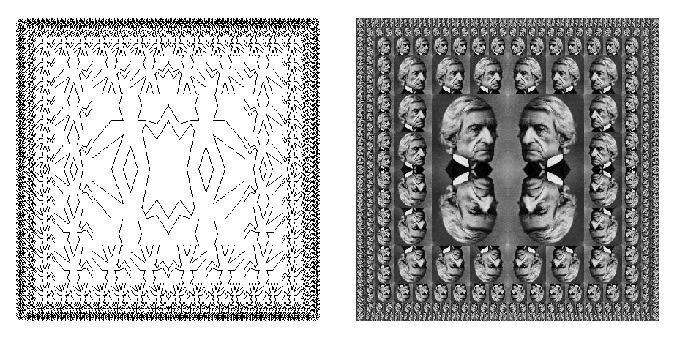
\includegraphics{xfig-mod/2-9.eps}
\caption{Узоры, порождаемые языком описания
изображений.}
\label{P2.9}

\end{cntrfig}

\paragraph{Язык описания изображений}


\index{ru}{язык описания изображений||picture language|||}\index{en}{picture language||язык описания изображений|||}
Когда в разделе~\ref{THE-ELEMENTS-OF-PROGRAMMING} мы начинали изучать 
программирование, мы подчеркивали важность описания языка через
рассмотрение его примитивов, методов комбинирования и методов
абстракции.  Мы будем следовать этой схеме и здесь.

Одно из элегантных свойств языка описания изображений
состоит в том, что в нем есть только один тип элементов, называемый
\index{ru}{рисовалка||painter|||}\index{en}{painter||рисовалка|||}{\em рисовалкой} (painter).  Рисовалка рисует
изображение с необходимым смещением и масштабом, чтобы попасть в
указанную 
\index{ru}{рамка||frame|||}\index{en}{frame||рамка|||}рамку в форме
параллелограмма.  Например, существует
элементарная рисовалка {\tt wave}, которая порождает грубую
картинку из линий, как показано на рисунке~\ref{P2.10}.
Форма изображения зависит от рамки ~--- все четыре изображения на
рисунке~\ref{P2.10} порождены одной и той же рисовалкой
{\tt wave}, но по отношению к четырем различным рамкам.
Рисовалки могут быть и более изощренными: элементарная рисовалка по
имени {\tt rogers} рисует портрет основателя MIT  Уильяма Бартона
Роджерса, как показано на рисунке~\ref{P2.11}\footnote{
  \index{ru}{MIT|ранняя история||||п}Уильям Бартон
  Роджерс\index{ru}{Роджерс, Уильям Бартон||William Barton
    Rogers||n|п}\index{en}{William Barton Rogers||Роджерс, Уильям
    Бартон||n|п} 
  (1804-1882) был основателем и первым
  президентом MIT.  Будучи геологом и способным педагогом, он преподавал 
  в Колледже Вильгельма и Марии, а также в университете штата Виргиния. В
  1859 году он переехал в Бостон, где у него было больше времени для
  исследований, разработал план создания <<политехнического института>>
  и служил первым Инспектором штата Массачусетс по газовым
  счетчикам.

  Когда в 1861 году был основан MIT, Роджерс был избран 
  его первым президентом.  Роджерс исповедовал идеал <<полезного
  обучения>>, отличного от университетского образования его времени с
  чрезмерным вниманием к классике, которое, как он писал, <<стояло
  на пути более широкого, высокого и практического обучения и
  преподавания в естественных и общественных науках>>. Это образование
  должно было отличаться и от узкого образования коммерческих школ. По
  словам Роджерса:

  \begin{quote}
    Повсеместно проводимое разделение между практическим
    и научным работником совершенно бесполезно, и весь опыт нашего
    времени показывает его полную несостоятельность.
  \end{quote}

  Роджерс был президентом MIT до 1870 года, когда он
  ушел в отставку по состоянию здоровья.  В 1878 году второй президент
  MIT Джон Ранкл\index{ru}{Ранкл, Джон Дэниел||John Daniel
    Runkle||n|п}\index{en}{John Daniel Runkle||Ранкл, Джон
    Дэниел||n|п}
  оставил свой пост из-за финансового кризиса, 
  вызванного биржевой паникой 1873 года, и напряженной борьбы с попытками 
  Гарварда поглотить MIT.  Роджерс вернулся и оставался на посту
  президента до 1881 года.

  Роджерс умер от приступа во время своей речи перед
  студентами MIT на выпускной церемонии 1882 года. В речи, посвященной
  его памяти и произнесенной в том же году, Ранкл приводит последние его слова:

  \begin{quote}
    <<Стоя здесь и видя, чем стал Институт, \ldots\ я
    вспоминаю о начале научных исследований.  Я вспоминаю, как сто
    пятьдесят лет назад Стивен Хейлс опубликовал статью на тему о светящемся 
    газе, где он утверждал, что его исследования показали, что 128 гран
    битумного угля\ldots>>

    \index{ru}{уголь, битумный||bituminous
      coal|||п}\index{en}{bituminous coal||уголь,
      битумный|||п}<<Битумный уголь>>~--- были его последние слова 
    в этом мире.  Он склонился вперед, как будто справляясь со своими
    заметками, которые лежали перед ним на столе, затем медленно
    выпрямился, поднял руки, и был перенесен со сцены своих земных забот и 
    триумфов в <<завтра смерти>>, где решены тайны жизни, и бестелесный
    дух находит неизмеримое наслаждение в созерцании новых и по-прежнему
    необъяснимых загадок бесконечного будущего.
  \end{quote}

  По словам  Фрэнсиса А. Уокера (третьего президента
  MIT):\index{ru}{Уокер, Фрэнсис Амаса||Francis Amasa
    Walker||n|п}\index{en}{Francis Amasa Walker||Уокер, Фрэнсис
    Амаса||n|п}

  \begin{quote}
    Всю свою жизнь он провел с огромной верой и
    героизмом, и умер так, как, наверное, и должен был желать столь
    превосходный рыцарь, в полном вооружении, на своем посту, и во время
    самого акта исполнения общественных обязанностей.
  \end{quote}}.
Четыре изображения на рисунке~\ref{P2.11} нарисованы относительно тех же
рамок, что и картинки {\tt wave} на рисунке~\ref{P2.10}.

При комбинировании изображений мы используем различные
\index{ru}{рисовалка|операции||||}
операции, которые строят новые рисовалки из рисовалок, полученных в
качестве аргументов.  Например, операция {\tt beside}
\index{ru}{beside||||p|}
получает
две рисовалки и порождает новую составную рисовалку, которая рисует
изображение первой рисовалки в левой половине рамки, а изображение
второй рисовалки в правой половине рамки.  Подобным образом,
{\tt below} 
\index{ru}{below||||p|}
принимает две рисовалки и порождает составную
рисовалку, рисующую изображение первого аргумента под изображением
второго аргумента.  Некоторые операции преобразуют одну рисовалку и
получают другую.  Например, {\tt flip-vert}
\index{ru}{flip-vert||||p|}
получает рисовалку и 
порождает новую, рисующую изображение вверх ногами, а
{\tt flip-horiz}
\index{ru}{flip-horiz||||p|}
порождает рисовалку, рисующую изображение
исходной в зеркальном отображении.


\begin{cntrfig}
\begin{tabular}{cc}
\input{p1.pictex} & \input{p4.pictex} \\
\input{p2.pictex} & \input{p3.pictex}
\end{tabular}
\caption{Изображения, порожденные рисовалкой
{\tt wave} по отношению к четырем различным рамкам.  Рамки,
показанные пунктиром, не являются частью изображений.}
\label{P2.10}

\end{cntrfig}

\begin{cntrfig}%раскомментарить по окончании работы
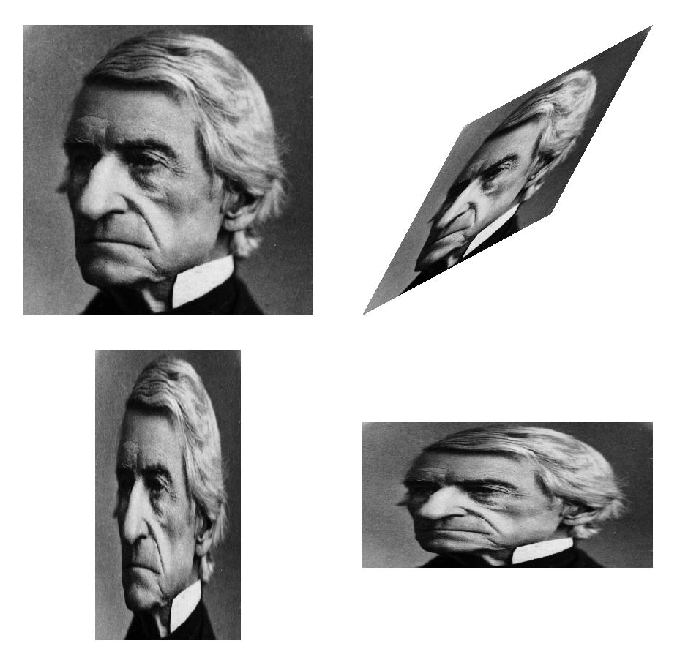
\includegraphics{xfig-mod/2-11.eps}
\caption{Изображения Уильяма Бартона Роджерса, основателя и первого президента MIT,
нарисованные по отношению к тем же четырем рамкам, что и на 
рисунке~\ref{P2.10} (первоначальное изображение печатается с
разрешения музея MIT).}
\label{P2.11}
\end{cntrfig}

На картинке \ref{P2.12} показан результат
работы рисовалки, называемой {\tt wave4}, который строится в
два этапа, начиная с {\tt wave}:

\begin{Verbatim}[fontsize=\small]
(define wave2 (beside wave (flip-vert wave)))
(define wave4 (below wave2 wave2))
\end{Verbatim}
Строя таким образом составные рисовалки, мы используем тот факт, что
\index{ru}{замыкание|свойство замыкания языка описания картинок||||}рисовалки замкнуты относительно средств комбинирования нашего
языка. {\tt Beside} или {\tt below} от двух рисовалок
само является рисовалкой; следовательно, мы можем ее использовать как
элемент при построении еще более сложных рисовалок.  Так же, как при
построении списковых структур с помощью {\tt cons}, замкнутость 
наших данных относительно средств комбинирования служит основой
способности строить сложные структуры при помощи всего лишь нескольких 
операций.

\begin{cntrfig}

\includegraphics{xfig-mod/2-12.eps}
\begin{Verbatim}
(define wave2                         (define wave4
  (beside wave (flip-vert wave)))       (below wave2 wave2))
\end{Verbatim}
\caption{Построение составного изображения,
начиная с рисовалки {\tt wave} с рисунка~\ref{P2.10}}
\label{P2.12}

\end{cntrfig}
Раз мы можем комбинировать рисовалки, нам хотелось бы
уметь выделять типичные схемы их комбинирования.  Операции над
рисовалками мы реализуем как процедуры языка Scheme. Это означает, что 
нам в языке изображений не требуется специального механизма
абстракции:  поскольку средства комбинирования являются обычными
процедурами Scheme, у нас автоматически есть право делать с операциями 
над рисовалками все то, что мы можем делать с процедурами.  Например,
схему построения {\tt wave4} мы можем абстрагировать в виде

\begin{Verbatim}[fontsize=\small]
(define (flipped-pairs painter)\index{ru}{flipped-pairs||||pd|}
  (let ((painter2 (beside painter (flip-vert painter))))
    (below painter2 painter2)))
\end{Verbatim}
и определить {\tt wave4} как пример применения этой схемы:

\begin{Verbatim}[fontsize=\small]
(define wave4 (flipped-pairs wave))
\end{Verbatim}

Мы можем определять и рекурсивные операции.  Вот пример,
который заставляет рисовалки делиться и ветвиться направо, как
показано на рисунках~\ref{P2.13} и \ref{P2.14}:
\looseness=-1

\begin{Verbatim}[fontsize=\small]
(define (right-split painter n)  \index{ru}{right-split||||pd|}
  (if (= n 0)
      painter
      (let ((smaller (right-split painter (- n 1))))
        (beside painter (below smaller smaller)))))
\end{Verbatim}
Можно порождать сбалансированные узоры, наращивая их не только направо, но
и вверх (см. упражнение~\ref{EX2.44} и рисунки~\ref{P2.13} и \ref{P2.14}):

\begin{Verbatim}[fontsize=\small]
(define (corner-split painter n)\index{ru}{corner-split||||pd|}
  (if (= n 0)
      painter
      (let ((up (up-split painter (- n 1)))
            (right (right-split painter (- n 1))))
        (let ((top-left (beside up up))
              (bottom-right (below right right))
              (corner (corner-split painter (- n 1))))
          (beside (below painter top-left)
                  (below bottom-right corner))))))
\end{Verbatim}
Соответствующим образом расположив четыре копии
{\tt corner-split}, мы получаем схему под названием
{\tt square-limit}, применение которой к {\tt wave} и
{\tt rogers} показано на рисунке~\ref{P2.9}:

\begin{Verbatim}[fontsize=\small]
(define (square-limit painter n)  \index{ru}{sqare-limit||||pd|}
  (let ((quarter (corner-split painter n)))
    (let ((half (beside (flip-horiz quarter) quarter)))
      (below (flip-vert half) half))))
\end{Verbatim}


\begin{cntrfig}
\begin{tabular}{|c|c|}
\hline
                            &  \\
                            &  {\tt right-split} \\
                            &  {\textit n}-1               \\
{\tt identity} &                         \\ \cline{2-2}     
                            & \\
                            &  {\tt right-split}      \\
                            &  {\textit n}-1 \\
                            &  \\                \hline
		
\multicolumn{2}{l}{{\tt right-split} \textit{n}}
\end{tabular}
\hspace{1cm}
\begin{tabular}{|c|c|c|}
\hline
                &             & \\
{\tt up-}        & {\tt up-}    & {\tt corner-split} \\
{\tt split}             & {\tt split}         & {\textit n}-1\\ 
{\textit n}-1                &  {\textit n}-1        &  \\              \hline
\multicolumn{2}{|c|}{}         &{\tt right-split} \\
\multicolumn{2}{|c|}{{\tt identity}} & {\textit n}-1 \\ \cline{3-3} 
\multicolumn{2}{|c|}{}       & {\tt right-split}\\
\multicolumn{2}{|c|}{}       & {\textit n}-1 \\
\hline
\multicolumn{3}{l}{\texttt{corner-split} \textit{n}}
\end{tabular}
\caption{Рекурсивные планы для
{\tt right-split} и {\tt corner-split}.}
\label{P2.13}

\end{cntrfig}


\begin{cntrfig}
\begin{tabular}{cc}
\multicolumn{2}{c}{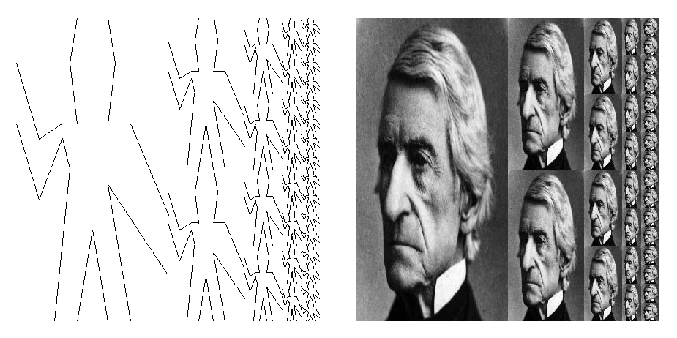
\includegraphics{xfig-mod/2-14-1.eps}} \\
\tt{(right-split wave 4)}  & \tt{(right-split rogers 4)}\\[8pt]
\multicolumn{2}{c}{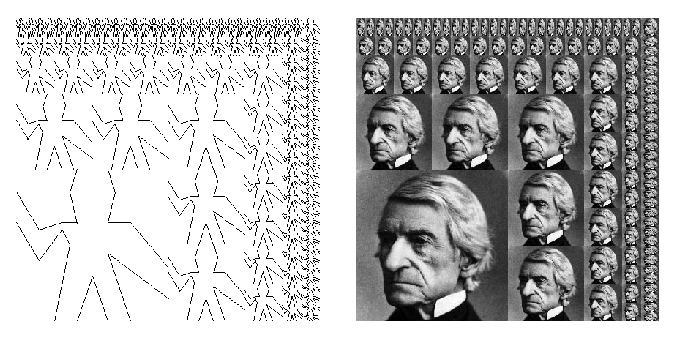
\includegraphics{xfig-mod/2-14-2.eps}} \\
\tt{(corner-split wave 4)} & \tt{(corner-split rogers 4)}
\end{tabular}

\caption{Рекурсивные операции
{\tt right-split} и {\tt corner-split} в применении к
рисовалкам {\tt wave} и {\tt rogers}. Комбинирование
четырех картинок {\tt corner-split} дает симметричные узоры
{\tt square-limit}, как показано на рисунке~\ref{P2.9}.}
\label{P2.14}
\end{cntrfig}

\begin{exercise}{2.44}\label{EX2.44}%
Определите процедуру \index{ru}{up-split||||p|(упр.~2.44)}{\tt up-split}, которую
использует {\tt corner-split}.  Она подобна
{\tt right-split}, но только меняет местами роли
{\tt below} и {\tt beside}.
\end{exercise}
\paragraph{Операции высших порядков}


\index{ru}{рисовалка|операции высших порядков||||}В дополнение к абстрагированию схем комбинирования
рисовалок, мы можем работать и на более высоком уровне, абстрагируя
схемы комбинирования операций над рисовалками. А именно, мы можем
рассматривать операции над рисовалками в качестве элементов, подлежащих
манипуляции, и писать средства комбинирования этих элементов ---
операции, которые принимают операции над рисовалками как аргументы и
создают новые операции.
\looseness=-1

Например, и {\tt flipped-pairs}, и
{\tt square-limit} располагают определенным образом в виде
квадрата четыре копии порождаемого рисовалкой изображения; они
отличаются только тем, как они ориентируют эти копии. Один из способов 
абстрагировать такую схему комбинирования рисовалок представлен
следующей процедурой, которая принимает четыре одноаргументных
операции и порождает операцию над рисовалками, которая трансформирует
данную ей рисовалку с помощью этих четырех операций и расставляет
результаты по квадрату. {\tt Tl}, {\tt tr},
{\tt bl} и {\tt br}~--- это трансформации, которые
следует применить к верхней левой, верхней правой, нижней левой и
нижней правой копиям, соответственно.
%\looseness=-1

\begin{Verbatim}[fontsize=\small]
(define (square-of-four tl tr bl br) \index{ru}{square-of-four||||pd|}
  (lambda (painter)
    (let ((top (beside (tl painter) (tr painter)))
          (bottom (beside (bl painter) (br painter))))
      (below bottom top))))
\end{Verbatim}


Тогда в терминах {\tt square-of-four} можно определить
{\tt flipped-pairs} следующим образом\footnote{Мы также могли бы написать

\begin{Verbatim}[fontsize=\footnotesize]
(define flipped-pairs\index{ru}{flipped-pairs||||pd|п}
  (square-of-four identity flip-vert identity flip-vert))
\end{Verbatim}
}:%%FOOTNOTE
\begin{Verbatim}[fontsize=\small]
(define (flipped-pairs painter)\index{ru}{flipped-pairs||||pd|}
  (let ((combine4 (square-of-four identity flip-vert
                                  identity flip-vert)))
    (combine4 painter)))
\end{Verbatim}
а {\tt square-limit} можно выразить как\footnote{{\tt Rotate180} поворачивает рисовалку на 180
градусов (см. упражнение~\ref{EX2.50}).  Вместо
{\tt rotate180} мы могли бы сказать {\tt (compose flip-vert
flip-horiz)}, используя процедуру {\tt compose} из
упражнения~\ref{EX1.42}.}

\begin{Verbatim}[fontsize=\small]
(define (square-limit painter n) \index{ru}{sqare-limit||||pd|}
  (let ((combine4 (square-of-four flip-horiz identity
                                  rotate180 flip-vert)))
    (combine4 (corner-split painter n))))
\end{Verbatim}
\begin{exercise}{2.45}\label{EX2.45}%
{\tt Right-split} и {\tt up-split} можно
выразить как разновидности общей операции разделения.  Определите
процедуру  \index{ru}{split||||p|(упр.~2.45)}{\tt split} с таким свойством, что вычисление

\begin{Verbatim}[fontsize=\small]
(define right-split (split beside below))
(define up-split (split below beside))
\end{Verbatim}
порождает процедуры {\tt right-split} и {\tt up-split} с 
таким же поведением, как и определенные ранее.
\end{exercise}

\paragraph{Рамки}\index{ru}{рамка|||||}

Прежде, чем мы сможем показать, как реализуются рисовалки 
и средства их комбинирования, нам нужно рассмотреть рамки.
Рамку можно описать как три \index{ru}{вектор (математический)|в кадре из языка описания изображений||||}вектора~--- вектор исходной точки и два вектора
краев рамки.  Вектор исходной точки $\mbox{\rm Origin}$ указывает смещение исходной точки 
рамки от некой абсолютной начальной точки, а векторы краев
$\mbox{\rm Edge}_1$ и $\mathop{\rm Edge}_2$
указывают смещение углов рамки от ее исходной точки.  Если края
перпендикулярны, рамка будет прямоугольной.  В противном случае рамка
будет представлять более общий случай параллелограмма.
На рис.~\ref{P2.15} показаны рамка и
соответствующие ей вектора.  В соответствии с принципами абстракции
данных, нам пока незачем указывать, каким образом представляются
рамки; нужно только сказать, что есть конструктор
{\tt make-frame},\index{ru}{make-frame||||p|}
который принимает три вектора и выдает рамку, 
и что есть еще три селектора, {\tt origin-frame},\index{ru}{origin-frame||||p|}
\index{ru}{edge1-frame||||p|}{\tt edge1-frame}
и {\tt edge2-frame}\index{ru}{edge2-frame||||p|}
(см. упражнение~\ref{EX2.47}).


\begin{cntrfig}
\input{xfig-mod/2-15.eepic}
%{\small вектор edge2 рамки\\
%вектор edge1 рамки\\
%вектор origin рамки\\
%точка (0,0) на экране дисплея}
\caption{Рамка представляется в виде трех векторов 
--- начальной точки и двух краев.}
\label{P2.15}

\end{cntrfig}

Для определения изображений мы будем использовать
координаты в 
\index{ru}{единичный квадрат||unit     square|||}\index{en}{unit     square||единичный квадрат|||}
единичном квадрате $(0 \le x, y \le
1)$. Каждой рамке мы сопоставляем 
\index{ru}{рамка|отображение координат||||}
\index{ru}{отображение координат рамки||frame coordinate map|||}\index{en}{frame coordinate map||отображение координат рамки|||}{\em отображение координат рамки} (frame coordinate map), которое будет
использоваться, чтобы сдвигать и масштабировать изображения так, чтобы 
они умещались в рамку.  Это отображение трансформирует единичный
квадрат в рамку, переводя вектор ${\bf v} = (x, y)$ в сумму 
векторов
$$
  \mathop{\rm Origin}(\mbox{\rm Frame}) 
    + x \cdot \mbox{\rm Edge}_1 (\mbox{\rm Frame})
    + y \cdot \mbox{\rm Edge}_2 (\mbox{\rm Frame})
$$
Например, (0, 0) отображается в исходную точку рамки, (1, 1) в
вершину, противоположную исходной точке по диагонали, а (0.5, 0.5) в
центр рамки. Мы можем создать отображение координат рамки при помощи
следующей процедуры\footnote{{\tt Frame-coord-map} использует векторные
операции, определенные ниже в упражнении~\ref{EX2.46}, и мы
предполагаем, что они реализованы для какого-нибудь представления
векторов.  Благодаря абстракции данных, неважно, каково это
представление; нужно только, чтобы операции над векторами вели себя
правильно.
}:

\begin{Verbatim}[fontsize=\small]
(define (frame-coord-map frame)\index{ru}{frame-coord-map||||pd|}
  (lambda (v)
    (add-vect
     (origin-frame frame)
     (add-vect (scale-vect (xcor-vect v)
                           (edge1-frame frame))
               (scale-vect (ycor-vect v)
                           (edge2-frame frame))))))
\end{Verbatim}
Заметим, что применение {\tt frame-coord-map} к рамке дает нам
процедуру, которая, получая вектор, возвращает тоже вектор.  Если
вектор-аргумент находится в единичном квадрате, вектор-результат
окажется в рамке. Например,

\begin{Verbatim}[fontsize=\small]
((frame-coord-map a-frame) (make-vect 0 0))
\end{Verbatim}
возвращает тот же вектор, что и 

\begin{Verbatim}[fontsize=\small]
(origin-frame a-frame)
\end{Verbatim}
\begin{exercise}{2.46}\label{EX2.46}%
Двумерный  \index{ru}{вектор (математический)|операции||||(упр.~2.46)}  \index{ru}{вектор (математический)|представленный в виде пары||||(упр.~2.46)}вектор ${\bf v}$, идущий от начала 
координат к точке, можно представить в виде пары, состоящей из
$x$-координаты и $y$-координаты.  Реализуйте
абстракцию данных для векторов, написав конструктор
{\tt make-vect}
\index{ru}{make-vect||||p|(упр.~2.46)}
и соответствующие селекторы
{\tt xcor-vect} 
\index{ru}{xcor-vect||||p|(упр.~2.46)}
и {\tt ycor-vect}. 
\index{ru}{ycor-vect||||p|(упр.~2.46)}
В терминах своих
селекторов и конструктора реализуйте процедуры {\tt add-vect},
\index{ru}{add-vect||||p|(упр.~2.46)}
{\tt sub-vect} и {\tt scale-vect}, которые выполняют
\index{ru}{sub-vect||||p|(упр.~2.46)}
\index{ru}{scale-vect||||p|(упр.~2.46)}
операции сложения, вычитания векторов и умножения вектора на скаляр:
$$
  \begin{array}{c}
    (x_1, y_1) + (x_2, y_2) = (x_1 + x_2, y_1 + y_2) \\
    (x_1, y_1) - (x_2, y_2) = (x_1 - x_2, y_1 - y_2) \\
    s \cdot (x, y) = (sx, sy) \\
  \end{array}
$$
\end{exercise}
\begin{exercise}{2.47}\label{EX2.47}%
Вот два варианта конструкторов для рамок:

\begin{Verbatim}[fontsize=\small]
(define (make-frame origin edge1 edge2)\index{ru}{make-frame||||pd|(упр.~2.47)}
  (list origin edge1 edge2))

(define (make-frame origin edge1 edge2)
  (cons origin (cons edge1 edge2)))
\end{Verbatim}
К каждому из этих конструкторов  добавьте соответствующие селекторы,
так, чтобы получить реализацию рамок.
\end{exercise}

\paragraph{Рисовалки}


\index{ru}{рисовалка|представление в виде процедуры||||} Рисовалка представляется в виде процедуры, которая,
получая в качестве аргумента рамку, рисует определенное изображение,
отмасштабированное и сдвинутое так, чтобы уместиться в эту рамку.  Это 
означает, что если есть рисовалка {\tt p} и рамка
{\tt f}, то мы можем получить изображение, порождаемое
{\tt p}, в {\tt f}, позвав {\tt p} с
{\tt f} в качестве аргумента.

Детали того, как реализуются элементарные рисовалки,
зависят от конкретных характеристик графической системы и типа
изображения, которое надо получить.  Например, пусть у нас будет
процедура {\tt draw-line},
\index{ru}{draw-line||||p|}
которая рисует на экране отрезок между 
двумя указанными точками.  Тогда мы можем создавать из списков
отрезков рисовалки для изображений, состоящих из этих отрезков, вроде рисовалки
{\tt wave} с рисунка~\ref{P2.10}, таким образом\footnote{Процедура {\tt segments->painter} использует
представление отрезков прямых, описанное ниже в упражнении~\ref{EX2.48}.  Кроме того, она использует
процедуру {\tt for-each}, описанную в упражнении~\ref{EX2.23}.
}:

\begin{Verbatim}[fontsize=\small]
(define (segments->painter segment-list)\index{ru}{segments->painter||||pd|}
  (lambda (frame)
    (for-each
     (lambda (segment)
       (draw-line
        ((frame-coord-map frame) (start-segment segment))
        ((frame-coord-map frame) (end-segment segment))))
     segment-list)))
\end{Verbatim}
Отрезки даются в координатах по отношению к единичному квадрату.  Для
каждого сегмента в списке рисовалка преобразует концы отрезка с
помощью отображения координат рамки и рисует отрезок между точками с
преобразованными координатами.

Представление рисовалок в виде процедур воздвигает в
языке построения изображений мощный барьер абстракции.  Мы можем
создавать и смешивать множество типов элементарных рисовалок, в
зависимости от имеющихся возможностей графики.  Детали их
реализации несущественны.  Любая процедура, если она принимает в
качестве аргумента рамку и рисует в ней что-нибудь должным образом
отмасштабированное, может служить рисовалкой\footnote{Например, рисовалка {\tt rogers} с 
рисунка~\ref{P2.11} была получена из полутонового черно-белого
изображения. Для каждой точки в указанной рамке рисовалка
{\tt rogers} определяет точку исходного изображения, которая в
нее отображается, и соответствующим образом ее окрашивает.  Разрешая 
себе иметь различные типы рисовалок, мы пользуемся идеей абстрактных
данных, описанной в разделе~\ref{WHAT-IS-MEANT-BY-DATA},
где мы говорили, что представление рациональных чисел может быть каким 
угодно, пока соблюдается соответствующее условие.  Здесь мы используем 
то, что рисовалку можно реализовать как угодно, лишь бы она что-то
изображала в указанной рамке.  В разделе~\ref{WHAT-IS-MEANT-BY-DATA} показывается и то,
как реализовать пары в виде процедур.  Рисовалки~--- это наш второй
пример процедурного представления данных.
}.
\begin{exercise}{2.48}\label{EX2.48}%
Направленный отрезок на плоскости можно представить в виде пары векторов:\index{ru}{отрезок|представление в виде пары векторов||||(упр.~2.48)}  вектор от начала координат до начала отрезка и
вектор от начала координат до конца отрезка.  Используйте свое
представление векторов из упражнения~\ref{EX2.46} и
определите представление отрезков с конструктором
{\tt make-segment}
\index{ru}{make-segment||||p|(упр.~2.48)}
и селекторами {\tt start-segment}
\index{ru}{start-segment||||p|(упр.~2.48)}
и {\tt end-segment}.
\index{ru}{end-segment||||p|(упр.~2.48)}
\end{exercise}
\begin{exercise}{2.49}\label{EX2.49}%
С помощью {\tt segments->painter} определите
следующие элементарные рисовалки:

\begin{plainenum}
\item
Рисовалку, которая обводит указанную рамку.

\item
Рисовалку, которая рисует <<Х>>, соединяя
противоположные концы рамки.

\item
Рисовалку, которая рисует ромб, соединяя между
собой середины сторон рамки.

\item
Рисовалку {\tt wave}.
\end{plainenum}
\end{exercise}

\paragraph{Преобразование и комбинирование рисовалок}


\index{ru}{рисовалка|преобразование и комбинирование||||}
Операции над рисовалками ({\tt flip-vert} или
{\tt beside}, например) создают новые рисовалки, которые
вызывает исходные рисовалки по отношению к рамкам, производным от
рамок-аргументов. Таким образом, скажем, {\tt flip-vert} не
требуется знать, как работает рисовалка, чтобы перевернуть ее ~--- ей
нужно только уметь перевернуть рамку вверх ногами: перевернутая
рисовалка просто использует исходную, но в обращенной рамке.

Операции над рисовалками основываются на процедуре
{\tt trans\-form-pain\-ter}, которая в качестве аргументов берет
рисовалку и информацию о том, как преобразовать рамку, а возвращает
новую рисовалку.  Когда преобразованная рисовалка вызывается по
отношению к какой-либо рамке, она преобразует рамку и вызывает
исходную рисовалку по отношению к ней.  Аргументами
{\tt transform-painter} служат точки (представленные в виде
векторов), указывающие углы новой рамки: будучи отображенной на рамку,
первая точка указывает исходную точку новой рамки, а две других~--- концы
краевых векторов.  Таким образом, аргументы, лежащие в пределах
единичного квадрата, определяют рамку, которая содержится внутри
исходной рамки.

\begin{Verbatim}[fontsize=\small]
(define (transform-painter painter origin corner1 corner2)\index{ru}{transform-painter||||pd|}
  (lambda (frame)
    (let ((m (frame-coord-map frame)))
      (let ((new-origin (m origin)))
        (painter
         (make-frame new-origin
                     (sub-vect (m corner1) new-origin)
                     (sub-vect (m corner2) new-origin)))))))
\end{Verbatim}

Вот как перевернуть изображение в рамке вертикально:

\begin{Verbatim}[fontsize=\small]
(define (flip-vert painter)\index{ru}{flip-vert||||pd|}
  (transform-painter painter
                     (make-vect 0.0 1.0)  {\em ; новая исходная точка}
                     (make-vect 1.0 1.0)  {\em ; новый конец {\tt edge1}}
                     (make-vect 0.0 0.0))){\em ; новый конец {\tt edge2}}
\end{Verbatim}
При помощи {\tt transform-painter} нам нетрудно будет определять
новые тран\-с\-формации.  Например, можно определить рисовалку, которая
рисует уменьшенную копию исходного изображения в верхней правой
четверти рамки:

\begin{Verbatim}[fontsize=\small]
(define (shrink-to-upper-right painter) \index{ru}{shrink-to-upper-right||||pd|}
  (transform-painter painter
                     (make-vect 0.5 0.5)
                     (make-vect 1.0 0.5)
                     (make-vect 0.5 1.0)))
\end{Verbatim}
Вот трансформация, которая поворачивает изображение
на 90 градусов против часовой стрелки\footnote{{\tt Rotate90} представляет собой чистый
поворот только для квадратных рамок, поскольку она еще растягивает и
сплющивает изображение так, чтобы оно уместилось в повернутой рамке.}:

\begin{Verbatim}[fontsize=\small]
(define (rotate90 painter)  \index{ru}{rotate90||||pd|}
  (transform-painter painter
                     (make-vect 1.0 0.0)
                     (make-vect 1.0 1.0)
                     (make-vect 0.0 0.0)))
\end{Verbatim}
А эта сжимает изображение по направлению к центру рамки\footnote{Ромбовидные изображения на рисунках~\ref{P2.10} и \ref{P2.11} были
получены с помощью {\tt squash-inwards}, примененной к
{\tt wave} и {\tt rogers}.}:

\begin{Verbatim}[fontsize=\small]
(define (squash-inwards painter) \index{ru}{squash-inwards||||pd|}
  (transform-painter painter
                     (make-vect 0.0 0.0)
                     (make-vect 0.65 0.35)
                     (make-vect 0.35 0.65)))
\end{Verbatim}

Преобразования рамок являются также основой для
определения средств комбинирования двух или более рисовалок.
Например, процедура {\tt beside} берет две рисовалки,
трансформирует их так, чтобы они работали соответственно в левой и
правой половинах рамки-аргумента, и создает новую составную
рисовалку.  Когда составной рисовалке передается рамка, она вызывает
первую из преобразованных рисовалок над левой половиной рамки, а
вторую над правой половиной:

\begin{Verbatim}[fontsize=\small]
(define (beside painter1 painter2)\index{ru}{beside||||pd|}
  (let ((split-point (make-vect 0.5 0.0)))
    (let ((paint-left
           (transform-painter painter1
                              (make-vect 0.0 0.0)
                              split-point
                              (make-vect 0.0 1.0)))
          (paint-right
           (transform-painter painter2
                              split-point
                              (make-vect 1.0 0.0)
                              (make-vect 0.5 1.0))))
      (lambda (frame)
        (paint-left frame)
        (paint-right frame)))))
\end{Verbatim}
Обратите внимание, как абстракция данных, и особенно представление
рисовалок в виде процедур, облегчает реализацию {\tt beside}.
Процедуре {\tt beside} не требуется ничего знать о деталях
рисовалок-компонент, кроме того, что каждая из них что-то изобразит в
указанной ей рамке.
\begin{exercise}{2.50}\label{EX2.50}%
Определите преобразование {\tt flip-horiz},
\index{ru}{flip-horiz||||p|(упр.~2.50)}
которое обращает изображение вокруг горизонтальной оси, а также
преобразования, которые вращают рисовалки против часовой стрелки на
180 и 270 градусов.
\end{exercise}
\begin{exercise}{2.51}\label{EX2.51}%
Определите для рисовалок операцию {\tt below}.
\index{ru}{below||||p|(упр.~2.51)}
{\tt Below} принимает в качестве аргументов две рисовалки.
Когда получившейся рисовалке передается рамка, она рисует в нижней ее
половине при помощи первой рисовалки, а в верхней при помощи второй.
Определите {\tt below} двумя способами~--- один раз аналогично
процедуре {\tt beside}, как она приведена выше, а второй раз
через {\tt beside} и операции вращения (см. упражнение~\ref{EX2.50}).
\end{exercise}

\paragraph{Уровни языка помогают устойчивому проектированию}


Язык построения изображений использует некоторые из
важнейших введенных нами идей, относящихся к абстракции
процедур и данных.  Базовая абстракция данных, рисовалки, реализуется
при помощи процедурного представления, и благодаря этому наш язык может
работать с различными графическими системами единым образом.  Средства 
комбинирования обладают свойством замыкания, и это позволяет нам легко 
возводить сложные построения.  Наконец, все средства абстракции
процедур доступны нам для того, чтобы абстрагировать средства
комбинирования рисовалок.

Нам удалось бросить взгляд и еще на одну существеннейшую
идею касательно проектирования языков и программ. Это подход 
\index{ru}{уровневое проектирование||stratified design|||}\index{en}{stratified design||уровневое проектирование|||}{\em уровневого проектирования} (stratified design),
представление, что сложной системе нужно придавать структуру при
помощи последовательности уровней, которая описывается
последовательностью языков.  Каждый из уровней строится путем
комбинации частей, которые на этом уровне рассматриваются как
элементарные, и части, которые строятся на каждом уровне,
работают как элементарные на следующем уровне.  Язык, который
используется на каждом уровне такого проекта, включает примитивы,
средства комбинирования и абстракции, соответствующие этому уровню
подробности.

Уровневое проектирование пронизывает всю технику
построения сложных систем.  Например, при проектировании компьютеров
резисторы и транзисторы сочетаются (и описываются при помощи языка
аналоговых схем), и из них строятся и-, или- элементы и им подобные,
служащие основой языка цифровых схем\footnote{Один из таких языков описывается в разделе~\ref{A-SIMULATOR-FOR-DIGITAL-CIRCUITS}.}.
Из этих элементов строятся процессоры, шины и системы памяти, которые
в свою очередь служат элементами в построении компьютеров при помощи 
языков, подходящих для описания компьютерной архитектуры.  Компьютеры, 
сочетаясь, дают распределенные системы, которые описываются при помощи 
языков описания сетевых взаимодействий, и так далее.

Как миниатюрный пример уровневого подхода, наш
язык описания изображений использует элементарные объекты (элементарные 
рисовалки), создаваемые при помощи языка, в котором описываются
точки и линии и создаются списки отрезков для рисовалки
{\tt segments->painter} либо градации серого цвета в рисовалке
вроде {\tt rogers}.  Большей частью наше описание языка
картинок было сосредоточено на комбинировании этих примитивов с
помощью геометрических комбинаторов вроде {\tt beside} и
{\tt below}.  Работали мы и на более высоком уровне, где
{\tt beside} и {\tt below} рассматривались как
примитивы, манипулируемые языком, операции которого, такие как
{\tt square-of-four}, фиксируют стандартные схемы сочетания
геометрических комбинаторов.

Уровневое проектирование помогает придать программам
\index{ru}{устойчивость программы||robustness|||}\index{en}{robustness||устойчивость программы|||}{\em устойчивость} (robus\-t\-ness), то есть повышает
вероятность, что небольшое изменение в спецификации потребует
относительно малых изменений в программе.  Например, предположим, что
нам нужно изменить картинку, основанную на рисовалке
{\tt wave}, которая показана на рисунке~\ref{P2.9}.  Мы
можем работать на самом низком уровне, изменяя конкретный вид элемента 
{\tt wave}; можем работать на промежуточном уровне и менять то, 
как {\tt corner-split} воспроизводит {\tt wave}; можем
на самом высоком уровне изменять то, как {\tt square-limit}
расставляет четыре копии по углам.  В общем, каждый уровень такого
проекта дает свой словарь для описания характеристик системы и свой
тип возможных изменений.
{\sloppy

}
\begin{exercise}{2.52}\label{EX2.52}%
Измените предел квадрата рисовалки {\tt wave}, 
показанный на рисунке~\ref{P2.9}, работая на каждом из
вышеописанных уровней. А именно:

\begin{plainenum}
\item
Добавьте новые отрезки к элементарной рисовалке
{\tt wave} из упражнения~\ref{EX2.49} (например,
изобразив улыбку).

\item
Измените шаблон, который порождает
{\tt corner-split} (например, используя то\-лько одну копию
образов {\tt up-split} и {\tt right-split} вместо двух).

\item
Измените версию {\tt square-limit},
использующую {\tt square-of-four}, так, чтобы углы
компоновались как-нибудь по-другому. (Например, можно сделать так, чтобы
большой мистер Роджерс выглядывал из каждого угла квадрата.)
\end{plainenum}
\end{exercise}

\section{Символьные данные}
\label{SYMBOLIC-DATA}


 \index{ru}{символ(ы)||symbol(s)|||}\index{en}{symbol(s)||символ(ы)|||}
Все составные объекты данных, которые мы до сих пор
использовали, состояли, в конечном счете, из чисел.  В этом 
разделе мы
расширяем возможности представления нашего языка, разрешая использовать
в качестве данных \index{ru}{данные|символьные||||}произвольные символы.

\subsection{Кавычки}
\label{QUOTATION}

\index{ru}{кавычки|||||}
Раз теперь нам можно формировать составные данные,
используя символы, мы можем пользоваться списками вроде

\begin{Verbatim}[fontsize=\small]
(a b c d)
(23 45 17)
((Norah 12) (Molly 9) (Anna 7) (Lauren 6) (Charlotte 3))
\end{Verbatim}
\index{ru}{Сассман, Джули Эстер Мазель, племянницы||nieces of Julie Esther Mazel Sussman||n|}\index{en}{nieces of Julie Esther Mazel Sussman||Сассман, Джули Эстер Мазель, племянницы||n|}
Списки, содержащие символы, могут выглядеть в точности как выражения
нашего языка:

\begin{Verbatim}[fontsize=\small]
(* (+ 23 45) (+ x 9))

(define (fact n) (if (= n 1) 1 (* n (fact (- n 1)))))
\end{Verbatim}

Чтобы работать с символами, нам в языке нужен новый
элемент: способность \index{ru}{кавычка||quote|||}\index{en}{quote||кавычка|||}{\em закавычить} (quote) объект
данных.  Допустим, нам хочется построить список {\tt (a b)}.
Этого нельзя добиться через {\tt (list a b)}, поскольку это
выражение строит список из {\em значений} символов
{\tt a} и {\tt b}, а не из них самих. Этот вопрос
хорошо изучен по отношению к естественным языкам, где слова и
предложения могут рассматриваться либо как семантические единицы,
либо как строки символов (синтаксические единицы). 
\index{ru}{естественный язык|кавычки|natural language|||}\index{en}{natural language||естественный язык|кавычки||} \index{ru}{кавычки|в естественном языке||||}В естественных языках обычно используют кавычки, чтобы обозначить, что  
слово или предложение нужно рассматривать буквально как строку
символов.  Например, первая буква <<Джона>>~--- разумеется,
<<Д>>.  Если мы говорим кому-то <<скажите, как Вас зовут>>, мы ожидаем
услышать имя этого человека.  Если же мы говорим кому-то <<скажите
``как Вас зовут''>>, то мы ожидаем услышать слова <<как Вас зовут>>.
Заметьте, как, для того, чтобы описать, что должен сказать кто-то другой, 
нам пришлось использовать кавычки\footnote{Когда мы разрешаем в языке кавычки, это разрушает нашу
способность говорить о языке в простых терминах, поскольку становится
неверным, что равнозначные выражения можно подставлять друг вместо
друга.  Например, три есть два плюс один, но слово <<три>> не есть
слова <<два плюс один>>.  Кавычки являются мощным инструментом,
поскольку они дают нам способ строить выражения, которые работают с
другими выражениями (как мы убедимся в главе~\ref{METALINGUISTIC-ABSTRACTION}, когда станем
писать интерпретатор).  Однако как только мы разрешаем в языке выражения,
которые говорят о других выражениях того же языка, становится очень
сложно соблюдать в каком-либо виде принцип <<равное можно
заменить равным>>.  Например, если мы знаем, что утренняя и вечерняя
звезда~--- одно и то же, то из утверждения  
\index{ru}{Венера||Venus|||п}\index{en}{Venus||Венера|||п}<<вечерняя
звезда~--- это Венера>> мы можем заключить, что <<утренняя звезда~---
это Венера>>. Однако если нам дано, что <<Джон знает, что вечерняя звезда~--- это
Венера>>, мы не можем заключить, что <<Джон знает, что утренняя звезда~--- это Венера>>.}.

Чтобы обозначать списки и символы, с которыми нужно
обращаться как с \index{ru}{кавычки|с объектами данных Лиспа||||}объектами данных, а не как с выражениями, которые
нужно вычислить, мы можем следовать тому же обычаю.  Однако наш
формат кавычек отличается от принятого в естественных языках тем, что мы ставим
знак кавычки (по традиции, это символ одинарной кавычки
{\tt '}) только в начале того объекта, который надо
закавычить.  В Scheme это сходит нам с рук, поскольку для разделения
объектов мы полагаемся на пробелы и скобки.  Таким образом, значением
одинарной кавычки является требование закавычить следующий
объект\footnote{\index{ru}{кавычки|одинарная
    vs. двойные||||п}Одинарная
кавычка отличается от двойной, которую мы
использовали для обозначения
\index{ru}{строка|печатание|string|||п}\index{en}{string||строка|печатание||п}\index{ru}{кавычки|со
  строкой символов||||п}
строк, выводимых на печать.  В то 
время как одинарную кавычку можно использовать для обозначения списков 
символов, двойная кавычка используется только со  строками, состоящими
из печатных знаков.  Единственное, для чего такие строки используются в 
нашей книге~--- это печать.\index{ru}{" (двойная
  кавычка)||||p|п}\index{ru}{' (одинарная кавычка)||||p|п}}.

 \index{ru}{символ(ы)|кавычки||||}Теперь мы можем отличать символы от их значений:

\begin{Verbatim}[fontsize=\small]
(define a 1)

(define b 2)

(list a b)
\textit{(1 2)}

(list 'a 'b)
\textit{(a b)}

(list 'a b)
\textit{(a 2)}
\end{Verbatim}

\index{ru}{список|кавычки||||}
Кроме того, кавычки позволяют нам вводить составные
объекты, используя обычное представление для печати списков:\footnote{Строго говоря, то, как мы используем кавычку, нарушает
общее правило, что все сложные выражения нашего языка должны
отмечаться скобками и выглядеть как списки.  Мы можем восстановить эту 
закономерность, введя особую форму \index{ru}{quote (особая форма)||||p|п} \index{ru}{особые формы|\texttt{quote}||||п}{\tt quote}, которая
служит тем же целям, что и кавычка.  Таким образом, мы можем печатать
{\tt (quote a)} вместо {\tt 'a} и {\tt (quote (a b
c))} вместо {\tt '(a b c)}. Именно так и работает
интерпретатор.  Знак кавычки~--- это просто сокращение, означающее,
что следующее выражение нужно завернуть в форму {\tt quote} и
получить {\tt (quote \textit{$\langle$выражение$\rangle$})}.  Это важно
потому, что таким образом соблюдается принцип, что с любым выражением,
которое видит интерпретатор, можно обращаться как с объектом
данных. Например, можно получить выражение {\tt (car '(a b
c))}, и это будет то же самое, что и {\tt (car (quote (a b
c)))}, вычислив {\tt (list 'car (list 'quote '(a b c)))}.}.

\begin{Verbatim}[fontsize=\small]
(car '(a b c))
\textit{a}

(cdr '(a b c))
\textit{(b c)}
\end{Verbatim}
Действуя в том же духе, пустой список мы можем получить, вычисляя
{\tt '()}, и таким образом избавиться от переменной
{\tt nil}.
\index{ru}{nil|избавление от|||p|}

Еще один примитив, который используется при 
работе с символами~--- это {\tt eq?},
\index{ru}{eq? (элементарная процедура)||||pd|}
\index{ru}{элементарные процедуры|{\tt eq?}||||} 
\index{ru}{символ(ы)|равенство||||}
который берет в качестве
аргументов два символа и проверяет, совпадают ли они\footnote{\index{ru}{равенство|символов||||п}Можно считать, что два символа <<совпадают>>, если они
состоят из одних и тех же печатных знаков в одинаковом порядке.  Такое
определение обходит важный вопрос, который мы пока не готовы
обсуждать: значение <<одинаковости>> в языке программирования.  К
нему мы вернемся в главе~\ref{MODULARITY-OBJECTS-AND-STATE} 
(раздел~\ref{THE-COSTS-OF-INTRODUCING-ASSIGNMENT}).}.

С помощью {\tt eq?} можно реализовать полезную процедуру,
называемую {\tt memq}. Она принимает два аргумента, символ и
список.  Если символ не содержится в списке (то есть, не равен в смысле 
{\tt eq?} ни одному из элементов списка), то
{\tt memq} возвращает ложь.  В противном случае она возвращает
подсписок списка, начиная с первого вхождения символа:

\begin{Verbatim}[fontsize=\small]
(define (memq item x)\index{ru}{memq||||pd|}
  (cond ((null? x) false)
        ((eq? item (car x)) x)
        (else (memq item (cdr x)))))
\end{Verbatim}
Например, значение

\begin{Verbatim}[fontsize=\small]
(memq 'apple '(pear banana prune))
\end{Verbatim}
есть ложь, в то время как значение

\begin{Verbatim}[fontsize=\small]
(memq 'apple '(x (apple sauce) y apple pear))
\end{Verbatim}
есть {\tt (apple pear)}.
\begin{exercise}{2.53}\label{EX2.53}%
Что напечатает интерпретатор в ответ на каждое из
следующих выражений?

\begin{Verbatim}[fontsize=\small]
(list 'a 'b 'c)

(list (list 'george))

(cdr '((x1 x2) (y1 y2)))

(cadr '((x1 x2) (y1 y2)))

(pair? (car '(a short list)))

(memq 'red '((red shoes) (blue socks)))

(memq 'red '(red shoes blue socks))
\end{Verbatim}
\end{exercise}
\begin{exercise}{2.54}\label{EX2.54}%
\index{ru}{список|равенство||||(упр.~2.54)}%
\index{ru}{равенство|списков||||(упр.~2.54)}%
Предикат {\tt equal?}\index{ru}{equal?||||p|(упр.~2.54)}
для двух списков возвращает
истину, если они содержат одни и те же элементы в одинаковом
порядке. Например,

\begin{Verbatim}[fontsize=\small]
(equal? '(this is a list) '(this is a list))
\end{Verbatim}
истинно, но

\begin{Verbatim}[fontsize=\small]
(equal? '(this is a list) '(this (is a) list))
\end{Verbatim}
ложно.  Более точно, можно определить {\tt equal?}
рекурсивно в терминах базового равенства символов {\tt eq?},
сказав, что {\tt a} равно {\tt b}, если оба они символы
и для них выполняется {\tt eq?} либо оба они списки и при этом
верно, что {\tt (car a)} равняется в смысле {\tt equal?} 
{\tt (car b)}, а {\tt (cdr a)} равняется в смысле 
{\tt equal?} {\tt (cdr b)}.  Пользуясь этой идеей, напишите 
{\tt equal?} в виде процедуры\footnote{На практике программисты используют
{\tt equal?} для\index{ru}{равенство|чисел||||п}\index{ru}{числа|равенство||||п}
сравнения не только символов, но и чисел.
Числа не считаются символами.  Вопрос о том, выполняется ли
{\tt eq?} для двух чисел, которые равны между собой (в смысле
{\tt =}), очень сильно зависит от конкретной реализации.  Более 
правильное определение {\tt equal?} (например, то, которое
входит в Scheme как элементарная процедура) должно содержать условие, что 
если и {\tt a}, и {\tt b} являются числами, то
{\tt equal?} для них выполняется тогда, когда они численно равны.}.
\end{exercise}

\begin{exercise}{2.55}\label{EX2.55}%
Ева Лу Атор вводит при работе с интерпретатором
выражение

\begin{Verbatim}[fontsize=\small]
(car ''abracadabra)
\end{Verbatim}
К ее удивлению, интерпретатор печатает {\tt quote}.  Объясните.
\end{exercise}

\subsection{Пример: символьное дифференцирование}
\label{EXAMPLE-SYMBOLIC-DIFFERENTIATION}


\index{ru}{дифференцирование|символьное||||}\index{ru}{символьное
  дифференцирование||symbolic differentiation|||}\index{en}{symbolic
  differentiation||символьное
  дифференцирование|||}\index{ru}{алгебраическое
  выражение|дифференцирование||||}Как иллюстрацию к понятию символьной
обработки, а также как дополнительный пример абстракции данных, 
рассмотрим построение процедуры,
которая производит символьное дифференцирование алгебраических
выражений.  Нам хотелось бы, чтобы эта процедура принимала в качестве
аргументов алгебраическое выражение и переменную, и чтобы она
возвращала производную выражения по отношению к этой переменной.
Например, если аргументами к процедуре служат $ax^2 + bx +
c$ и $x$, процедура должна возвращать $2ax +
b$.  Символьное дифференцирование имеет для Лиспа особое
историческое значение.  Оно было одним из побудительных примеров при
разработке компьютерного языка для обработки символов.  Более того,
оно послужило началом линии исследований, приведшей к разработке 
мощных систем для символической математической работы, которые сейчас
все больше используют прикладные математики и физики.

При разработке программы для символьного дифференцирования
мы будем следовать той же самой стратегии абстракции данных, согласно
которой мы действовали при разработке системы рациональных чисел в
разделе~\ref{EXMP-ARITH-OPER-FOR-RAT-NUMBERS}.
А именно, сначала мы разработаем алгоритм дифференцирования, который
работает с абстрактными объектами, такими как <<суммы>>,
<<произведения>> и <<переменные>>, не обращая внимания на то, как они
должны быть представлены.  Только после этого мы обратимся к задаче
представления.

\paragraph{Программа дифференцирования с абстрактными
данными}


Чтобы упростить задачу, мы рассмотрим простую программу
\index{ru}{дифференцирование|правила||||} 
символьного дифференцирования, которая работает с выражениями,
построенными только при помощи операций сложения и умножения с двумя
аргументами.  Дифференцировать любое такое выражение можно, применяя
следующие правила редукции:
$$
   \frac{dc}{dx} = 0\ \mbox{\rm для константы либо переменной, отличной 
от $x$}
$$

$$
  \frac{dx}{dx} = 1
$$

$$
  \frac{d(u+v)}{dx} = \frac{du}{dx} + \frac{dv}{dx}
$$

$$
  \frac{d(uv)}{dx} = u (\frac{dv}{dx}) + v (\frac{du}{dx})
$$

Заметим, что два последних правила по сути своей
рекурсивны. То есть, чтобы получить производную суммы, нам сначала
нужно получить производные слагаемых и их сложить.  Каждое из них в
свою очередь может быть выражением, которое требуется разложить на 
составляющие.  Разбивая их на все более мелкие части, мы в конце концов 
дойдем до стадии, когда все части являются либо константами, либо 
переменными, и их производные будут равны либо 0, либо 1.

Чтобы воплотить эти правила в виде процедуры, мы позволим
себе немного  \index{ru}{мечтать не вредно|||||}помечтать, 
подобно тому, как мы делали при реализации
рациональных чисел. Если бы у нас был способ представления
алгебраических выражений, мы могли бы проверить, является ли выражение 
суммой, произведением, константой или переменной. Можно было бы
извлекать части выражений.  Например, для суммы мы хотели бы уметь
получать первое и второе слагаемое.  Еще нам нужно уметь составлять
выражения из частей.  Давайте предположим, что у нас уже есть
процедуры, которые реализуют следующие селекторы, конструкторы и
предикаты:

\begin{plainlist}

\item
{\bf {\tt (variable? e)}} \index{ru}{variable?||||p|}
Является ли {\tt e} переменной?
\item
{\bf {\tt (same-variable? v1 v2)}} \index{ru}{same-variable?||||p|}
Являются ли {\tt v1} и {\tt v2}
одной и той же переменной?
\item
{\bf {\tt (sum? e)}} \index{ru}{sum?||||p|}
Является ли {\tt e} суммой?
\item
{\bf {\tt (addend e)}} \index{ru}{addend||||p|}
Первое слагаемое суммы {\tt e}.
\item
{\bf {\tt (augend e)}} \index{ru}{augend||||p|}
Второе слагаемое суммы {\tt e}.
\item
{\bf {\tt (make-sum a1 a2)}} \index{ru}{make-sum||||p|}
Строит сумму {\tt a1} и {\tt a2}.
\item
{\bf {\tt (product? e)}} \index{ru}{product?||||p|}
Является ли {\tt e} произведением?
\item
{\bf {\tt (multiplier e)}} Первый множитель произведения {\tt e}.
\item
{\bf {\tt (multiplicand e)}} Второй множитель произведения {\tt e}.
\item
{\bf {\tt (make-product m1 m2)}} \index{ru}{make-product||||p|}
Строит произведение {\tt m1} и {\tt m2}.
\end{plainlist}
При помощи этих процедур и элементарного предиката
{\tt number?}, 
\index{ru}{number? (элементарная процедура)||||pd|}
\index{ru}{элементарные процедуры|{\tt number}||||} 
который распознает числа, мы можем выразить
правила дифференцирования в виде следующей процедуры:

\begin{Verbatim}[fontsize=\small]
(define (deriv exp var)\index{ru}{deriv (символическая)||||pd|}
  (cond ((number? exp) 0)
        ((variable? exp)
         (if (same-variable? exp var) 1 0))
        ((sum? exp)
         (make-sum (deriv (addend exp) var)
                   (deriv (augend exp) var)))
        ((product? exp)
         (make-sum
           (make-product (multiplier exp)
                         (deriv (multiplicand exp) var))
           (make-product (deriv (multiplier exp) var)
                         (multiplicand exp))))
        (else
         (error "неизвестный тип выражения -- DERIV" exp))))
\end{Verbatim}
Процедура {\tt deriv} заключает в себе весь алгоритм
дифференцирования.  Поскольку она выражена в терминах
абстрактных данных, она будет работать, как бы мы ни представили
алгебраические выражения, если только у нас будут соответствующие
селекторы и конструкторы.  Именно этим вопросом нам и нужно теперь
заняться.

\paragraph{Представление алгебраических выражений}


Можно представить себе множество способов представления
алгебраических выражений с помощью списковых структур. Например, можно 
использовать списки символов, которые отражали бы обычную
алгебраическую нотацию, так что $ax + b$ представлялось бы
как список {\tt (a * x + b)}.  Однако естественней всего
использовать ту же скобочную префиксную запись, с помощью которой в
Лиспе представляются комбинации; то есть представлять $ax +
b$ в виде {\tt (+ (* a x) b)}.  Тогда наше представление
данных для задачи дифференцирования будет следующим:
\index{ru}{алгебраическое выражение|представление||||}

\begin{plainlist}


\item
Переменные~--- это символы.  Они распознаются
элементарным предикатом {\tt symbol?}: \index{ru}{элементарные процедуры|{\tt symbol?}||||}  \index{ru}{symbol? (элементарная процедура)||||pd|}

\begin{Verbatim}[fontsize=\small]
(define (variable? x) (symbol? x))
\end{Verbatim}

\item
Две переменные одинаковы, если для представляющих
их символов выполняется {\tt eq?}:

\begin{Verbatim}[fontsize=\small]
(define (same-variable? v1 v2)  \index{ru}{same-variable?||||pd|}
  (and (variable? v1) (variable? v2) (eq? v1 v2)))
\end{Verbatim}

\item
Суммы и произведения конструируются как списки:

\begin{Verbatim}[fontsize=\small]
(define (make-sum a1 a2) (list '+ a1 a2))\index{ru}{make-sum||||pd|}

(define (make-product m1 m2) (list '* m1 m2))\index{ru}{make-product||||pd|}
\end{Verbatim}

\item
Сумма~--- это список, первый элемент которого
символ {\tt +}:

\begin{Verbatim}[fontsize=\small]
(define (sum? x)  \index{ru}{sum?||||pd|}
  (and (pair? x) (eq? (car x) '+)))
\end{Verbatim}

\item
Первое слагаемое~--- это второй элемент списка,
представляющего сумму:

\begin{Verbatim}[fontsize=\small]
(define (addend s) (cadr s))\index{ru}{addend||||pd|}
\end{Verbatim}

\item
Второе слагаемое~--- это третий элемент списка,
представляющего сумму:

\begin{Verbatim}[fontsize=\small]
(define (augend s) (caddr s))\index{ru}{augend||||pd|}
\end{Verbatim}

\item
Произведение~--- это список, первый элемент
которого символ {\tt *}:

\begin{Verbatim}[fontsize=\small]
(define (product? x)  \index{ru}{product?||||pd|}
  (and (pair? x) (eq? (car x) '*)))
\end{Verbatim}

\item
Первый множитель~--- это второй элемент списка,
представляющего произведение:

\begin{Verbatim}[fontsize=\small]
(define (multiplier p) (cadr p))\index{ru}{multiplier|селектор|||pd|}
\end{Verbatim}

\item
Второй множитель~--- это третий элемент списка,
представляющего произведение:

\begin{Verbatim}[fontsize=\small]
(define (multiplicand p) (caddr p))\index{ru}{multiplicand||||pd|}
\end{Verbatim}
\end{plainlist}
Таким образом, нам осталось только соединить это представление с
алгоритмом, заключенным в процедуре {\tt deriv}, и мы получаем
работающую программу символьного дифференцирования.  Посмотрим на
некоторые примеры ее поведения:

\begin{Verbatim}[fontsize=\small]
(deriv '(+ x 3) 'x)
\textit{(+ 1 0)}

(deriv '(* x y) 'x)
\textit{(+ (* x 0) (* 1 y))}

(deriv '(* (* x y) (+ x 3)) 'x)
\textit{(+ (* (* x y) (+ 1 0))}
   \textit{(* (+ (* x 0) (* 1 y))}
      \textit{(+ x 3)))}
\end{Verbatim}
Ответы, которые выдает программа, правильны; однако их нужно
упрощать.  Верно, что
$$
  \frac{d(xy)}{dx} = x \cdot 0 + 1 \cdot y
$$
но нам хотелось бы, чтобы программа знала, что $x \cdot 0 =
0$, $1 \cdot y = y$, а $0 + y =
y$. Ответом на второй пример должно быть просто $y$.
Как видно из третьего примера, при усложнении выражений упрощение 
превращается в серьезную проблему.

\index{ru}{упрощение алгебраических выражений||simplification of algebraic    expressions|||}\index{en}{simplification of algebraic    expressions||упрощение алгебраических выражений|||}
\index{ru}{алгебраическое выражение|упрощение||||}
Наши теперешние затруднения очень похожи на те, с которыми 
мы столкнулись при реализации рациональных чисел: мы не привели ответы к 
простейшей форме.  Чтобы произвести приведение рациональных чисел, нам 
потребовалось изменить только конструкторы и селекторы в нашей
реализации.  Здесь мы можем применить подобную же стратегию.
Процедуру {\tt deriv} мы не будем изменять вовсе.  Вместо этого 
мы изменим {\tt make-sum} так, что если оба слагаемых являются
числами, она их сложит и вернет их сумму.  Кроме того, если одно из
слагаемых равно 0, то {\tt make-sum} вернет другое.

\begin{Verbatim}[fontsize=\small]
(define (make-sum a1 a2)
  (cond ((=number? a1 0) a2)
        ((=number? a2 0) a1)
        ((and (number? a1) (number? a2)) (+ a1 a2))
        (else (list '+ a1 a2))))
\end{Verbatim}
Здесь используется процедура {\tt =number?}, которая проверяет, 
не равно ли выражение определенному числу:

\begin{Verbatim}[fontsize=\small]
(define (=number? exp num)\index{ru}{=number?||||pd|}
  (and (number? exp) (= exp num)))
\end{Verbatim}
Подобным же образом мы изменим и {\tt make-product}, так. чтобы 
встроить в него правила, что нечто, умноженное на 0, есть 0, а
умноженное на 1 равно самому себе:

\begin{Verbatim}[fontsize=\small]
(define (make-product m1 m2)
  (cond ((or (=number? m1 0) (=number? m2 0)) 0)
        ((=number? m1 1) m2)
        ((=number? m2 1) m1)
        ((and (number? m1) (number? m2)) (* m1 m2))
        (else (list '* m1 m2))))
\end{Verbatim}
Вот как эта версия работает на наших трех примерах:

\begin{Verbatim}[fontsize=\small]
(deriv '(+ x 3) 'x)
\textit{1}

(deriv '(* x y) 'x)
\textit{y}

(deriv '(* (* x y) (+ x 3)) 'x)
\textit{(+ (* x y) (* y (+ x 3)))}
\end{Verbatim}
Хотя это заметное улучшение, третий пример показывает, что нужно
многое еще сделать, прежде чем мы получим программу, приводящую
выражения к форме, которую мы согласимся считать <<простейшей>>.
Задача алгебраического упрощения сложна, среди прочего, еще и потому,
что форма, которая является простейшей для одних целей, может таковой
не являться для других.
\begin{exercise}{2.56}\label{EX2.56}%
\index{ru}{дифференцирование|правила||||(упр.~2.56)}%
Покажите, как расширить простейшую программу
дифференцирования так, чтобы она воспринимала больше разных типов 
выражений.  Например, реализуйте правило взятия производной
$$
  \frac{d(u^n)}{dx} = n u^{n-1} (\frac{du}{dx})
$$
добавив еще одну проверку к программе {\tt deriv} и определив
соответствующие процедуры {\tt exponentiation?},
{\tt base}, {\tt exponent} и
{\tt make-exponentiation} (обозначать возведение в степень
можно символом {\tt **}).  Встройте правила, что любое выражение,
возведенное в степень 0, дает 1, а возведенное в степень 1 равно
самому себе.
\end{exercise}
\begin{exercise}{2.57}\label{EX2.57}%
Расширьте программу дифференцирования так, чтобы она
работала с суммами и произведениями любого (больше двух) количества
термов.  Тогда последний из приведенных выше примеров мог бы быть записан 
как

\begin{Verbatim}[fontsize=\small]
(deriv '(* x y (+ x 3)) 'x)
\end{Verbatim}
Попытайтесь сделать это, изменяя только представление сумм и
произведений, не трогая процедуру {\tt deriv}.  Тогда,
например, процедура {\tt addend} будет возвращать первое
слагаемое суммы, а {\tt augend} сумму остальных.
\end{exercise}
\begin{exercise}{2.58}\label{EX2.58}%
\index{ru}{инфиксная нотация vs. префиксная нотация||infix notation vs. prefix notation|||(упр.~2.58)}%
\index{en}{infix notation vs. prefix notation||инфиксная нотация vs. префиксная нотация|||(упр.~2.58)}%  
\index{ru}{префиксная нотация|vs. инфиксная нотация||||(упр.~2.58)}%
Предположим, что нам захотелось изменить программу
дифференцирования так, чтобы она работала с обычной математической
нотацией, где {\tt +} и {\tt *} не префиксные, а
инфиксные операции.  Поскольку программа взятия производных определена 
в терминах абстрактных данных, мы можем изменять представление
выражений, с которыми она работает, меняя только предикаты, селекторы
и конструкторы, определяющие представление алгебраических
выражений, с которыми должен работать дифференциатор.

\begin{plainenum}
\item
Покажите, как это сделать так, чтобы брать
производные от выражений, представленных в инфиксной форме, например
{\tt (x + (3 * (x + (y + 2))))}.  Для упрощения задачи
предположите, что {\tt +} и {\tt *} всегда принимают по
два аргумента, и что в выражении расставлены все скобки.

\item
 Задача становится существенно сложней, если мы
разрешаем стандартную алгебраическую нотацию, например
{\tt (x + 3 * (x + y + 2))}, которая опускает ненужные скобки и 
предполагает, что умножение выполняется раньше, чем сложение.  Можете
ли Вы разработать соответствующие предикаты, селекторы и конструкторы
для этой нотации так, чтобы наша программа взятия производных
продолжала работать?
\end{plainenum}
\end{exercise}

\subsection{Пример: представление множеств}
\label{EXAMPLE-REPRESENTING-SETS}

\index{ru}{множество|||||}%
В предыдущих примерах мы построили представления для двух
типов составных объектов: для рациональных чисел и для алгебраических
выражений.  В одном из этих примеров перед нами стоял выбор, упрощать
ли выражение при его конструировании или при обращении; в остальном же
выбор представления наших структур через списки был простым делом.
Когда мы обращаемся к представлению множеств, выбор представления не
так очевиден.  Здесь существует несколько возможных представлений, и
они значительно отличаются друг от друга в нескольких аспектах.

Говоря неформально, множество есть просто набор различных
объектов.  Чтобы дать ему более точное определение, можно использовать 
метод абстракции данных.  А именно, мы определяем <<множество>>, указывая
\index{ru}{множество|операции||||}операции, которые можно производить над
множествами.  Это операции {\tt union-set} (объединение),
{\tt intersection-set} (пересечение),\index{ru}{intersection-set||||p|}
{\tt element-of-set?} (проверка на принадлежность) и
{\tt adjoin-set} (добавление элемента).\index{ru}{adjoin-set||||p|}
{\tt Element-of-set?}\index{ru}{element-of-set?||||p|}
--- это предикат, который определяет,
является ли данный объект элементом множества. {\tt Adjoin-set}
принимает как аргументы объект и множество, и возвращает множество,
которое содержит все элементы исходного множества плюс добавленный
элемент. \index{ru}{union-set||||p|}{\tt Union-set} вычисляет объединение двух множеств,
то есть множество, содержащее те элементы, которые присутствуют хотя
бы в одном из аргументов.  {\tt Intersection-set} вычисляет
пересечение двух множеств, то есть множество, которое содержит только 
те элементы, которые присутствуют в обоих аргументах.  С точки зрения
абстракции данных, мы имеем право взять любое
представление, позволяющее нам использовать эти операции способом, который
согласуется с вышеуказанной интерпретацией\footnote{\samepage%
Если нам хочется быть более формальными, мы можем
определить <<соответствие вышеуказанной интерпретации>> как условие,
что операции удовлетворяют некоторому набору правил вроде
следующих:

\begin{plainlist}
\item
Для любого множества {\tt S} и любого
объекта {\tt x}, {\tt (element-of-set? x (adjoin-set x
S))} истинно (неформально: <<добавление объекта к множеству дает 
множество, содержащее этот объект>>).

\item
Для любых двух множеств {\tt S} и
{\tt T} и любого объекта {\tt x}, {\tt (element-of-set?
x (union-set S T))} равно {\tt (or (element-of-set? x S)
(element-of-set? x T))} (неформально: <<элементы {\tt (union-set S
T)}~--- это те элементы, которые принадлежат либо
{\tt S}, либо {\tt T}>>).

\item
Для любого объекта {\tt x},
{\tt (element-of-set? x '())} ложно (неформально: <<ни один 
объект не принадлежит пустому множеству>>).
\end{plainlist}}.

\paragraph{Множества как неупорядоченные списки }


\index{ru}{множество|представленное в виде    неупорядоченного списка||||}  
\index{ru}{представление множеств в виде неупорядоченных     списков||unordered-list repre\-sen\-ta\-tion of sets|||}\index{en}{unordered-list repre\-sen\-ta\-tion of sets||представление множеств в виде неупорядоченных     списков|||}
Можно представить множество как список, в котором ни один 
элемент не содержится более одного раза.  Пустое множество
представляется пустым списком.  При таком представлении
{\tt element-of-set?} подобен процедуре {\tt memq} из
раздела~\ref{QUOTATION}.  Она использует не
{\tt eq?}, а {\tt equal?}, так что элементы множества не 
обязаны быть символами:

\begin{Verbatim}[fontsize=\small]
(define (element-of-set? x set)\index{ru}{element-of-set?|представление в виде неупорядоченных списков|||pd|}
  (cond ((null? set) false)
        ((equal? x (car set)) true)
        (else (element-of-set? x (cdr set)))))
\end{Verbatim}
Используя эту процедуру, мы можем написать
{\tt adjoin-set}. Если объект, который требуется добавить, уже
принадлежит множеству, мы просто возвращаем исходное множество.  В
противном случае мы используем {\tt cons}, чтобы добавить
объект к списку. представляющему множество:

\begin{Verbatim}[fontsize=\small]
(define (adjoin-set x set)\index{ru}{adjoin-set|представление в виде неупорядоченных списков|||pd|}
  (if (element-of-set? x set)
      set
      (cons x set)))
\end{Verbatim}
Для {\tt intersection-set} можно использовать рекурсивную
стратегию.  Если мы знаем, как получить пересечение {\tt set2} и 
{\tt cdr} от {\tt set1}, нам нужно только понять, надо
ли добавить к нему {\tt car} от {\tt set1}.  Это зависит 
от того, принадлежит ли {\tt (car set1)} еще и
{\tt set2}.  Получается такая процедура:

\begin{Verbatim}[fontsize=\small]
(define (intersection-set set1 set2)\index{ru}{intersection-set|представление в виде неупорядоченных списков|||pd|}
  (cond ((or (null? set1) (null? set2)) '())
        ((element-of-set? (car set1) set2)
         (cons (car set1)
               (intersection-set (cdr set1) set2)))
        (else (intersection-set (cdr set1) set2))))
\end{Verbatim}

Один из вопросов, которые должны нас заботить при
разработке реализации~--- эффективность.  Рассмотрим число шагов,
которые требуют наши операции над множествами.  Поскольку все они
используют {\tt element-of-set?}, скорость этой операции
оказывает большое влияние на скорость реализации в целом.  Теперь
заметим, что для того, чтобы проверить, является ли объект элементом
множества, процедуре {\tt element-of-set?} может потребоваться
просмотреть весь список. (В худшем случае оказывается, что объекта в
списке нет.)  Следовательно, если в множестве $n$
элементов,  {\tt element-of-set?} может затратить до
$n$ шагов.  Таким образом, число требуемых шагов растет как 
$\Theta (n)$.  Число шагов, требуемых
{\tt adjoin-set}, которая эту операцию использует, также растет 
как $\Theta (n)$.  Для {\tt intersection-set},
которая проделывает {\tt element-of-set?} для каждого элемента
{\tt set1}, число требуемых шагов растет как произведение
размеров исходных множеств, или $\Theta (n^2)$ для двух
множеств размера $n$.  То же будет верно и для
{\tt union-set}.
\begin{exercise}{2.59}\label{EX2.59}%
Реализуйте операцию \index{ru}{union-set|представление в виде неупорядоченных списков|||p|(упр.~2.59)} {\tt union-set} для
представления множеств в виде неупорядоченных списков.
\end{exercise}
\begin{exercise}{2.60}\label{EX2.60}%
Мы указали, что множество представляется как список без 
повторяющихся элементов. Допустим теперь, что мы разрешаем
повторяющиеся элементы. Например, множество $\{1, 2, 3\}$
могло бы быть представлено как список {\tt (2 3 2 1 3 2 2)}.
Разработайте процедуры {\tt element-of-set?},
{\tt adjoin-set}, {\tt union-set} и
{\tt intersection-set}, которые бы работали с таким
представлением.  Как соотносится эффективность этих операций с
эффективностью соответствующих процедур для представления без
повторений?  Существуют ли приложения, в которых Вы бы использовали
скорее это представление, чем представление без повторений?
\end{exercise}

\paragraph{Множества как упорядоченные списки}


\index{ru}{представление множеств в виде    упорядоченных списков||ordered-list    repre\-sen\-ta\-tion of sets|||}\index{en}{ordered-list  re\-pre\-sen\-ta\-tion of sets||представление множеств в виде    упорядоченных списков|||} 
\index{ru}{множество|представленное в виде упорядоченного списка||||}
Один из способов ускорить операции над множествами
состоит в том, чтобы изменить представление таким образом, чтобы
элементы множества перечислялись в порядке возрастания.  Для этого
нам потребуется способ сравнения объектов, так, чтобы
можно было сказать, какой из них больше.  Например, символы мы могли
бы сравнивать лексикографически, или же мы могли бы найти какой-нибудь 
способ ставить каждому объекту в соответствие некоторое уникальное
число и затем сравнивать объекты путем сравнения соответствующих
чисел.  Чтобы упростить обсуждение, мы рассмотрим только случай, когда 
элементами множества являются числа, так что мы сможем сравнивать
элементы при помощи {\tt >} и {\tt <}.  Мы будем 
представлять множество чисел как список его элементов в возрастающем
порядке.  В то время как первая наша реализация позволяла нам
представлять множество $\{1, 3, 6, 10\}$ путем перечисления 
его элементов в произвольном порядке, в новом представлении разрешен
только список {\tt (1 3 6 10)}.

Одно из преимуществ упорядочения проявляется в
{\tt element-of-set?}: проверяя наличие элемента, нам больше
незачем просматривать все множество.  Если мы достигли элемента,
который больше того объекта, который мы ищем, мы можем уже сказать,
что искомого в списке нет:

\begin{Verbatim}[fontsize=\small]
(define (element-of-set? x set)\index{ru}{element-of-set?|представление в виде упорядоченных списков|||pd|}
  (cond ((null? set) false)
        ((= x (car set)) true)
        ((< x (car set)) false)
        (else (element-of-set? x (cdr set)))))
\end{Verbatim}
Сколько шагов мы на этом выигрываем? В худшем случае, объект, который
мы ищем, может быть наибольшим в множестве, так что число шагов то же, 
что и для неупорядоченного представления.  С другой стороны, если мы
ищем элементы разных размеров, можно ожидать, что иногда мы сможем
останавливаться близко к началу списка, а иногда нам все же
потребуется просмотреть большую его часть.  В среднем мы можем
ожидать, что потребуется просмотреть около половины элементов
множества.  Таким образом, среднее число требуемых шагов будет
примерно $n / 2$. Это все еще рост порядка $\Theta 
(n)$, но это экономит нам в среднем половину числа шагов по 
сравнению с предыдущей реализацией.
\looseness=-1

Более впечатляющее ускорение мы получаем в
{\tt intersection-set}.  При неупорядоченном представлении эта
операция требовала $\Theta (n^2)$ шагов, поскольку мы
производили полный поиск  в {\tt set2} для каждого элемента
{\tt set1}.  Однако при упорядоченном представлении мы можем
воспользоваться более разумным методом.  Начнем со сравнения первых
элементов двух множеств, {\tt x1} и {\tt x2}.  Если
{\tt x1} равно {\tt x2}, мы получаем один элемент
пересечения, а остальные элементы пересечения мы можем получить,
пересекая оставшиеся элементы списков-множеств.  Допустим, однако, что 
{\tt x1} меньше, чем {\tt x2}.  Поскольку
{\tt x2}~--- наименьший элемент {\tt set2}, мы можем
немедленно заключить, что {\tt x1} больше нигде в
{\tt set2} не может встретиться и, следовательно, не
принадлежит пересечению.  Следовательно пересечение двух множеств
равно пересечению {\tt set2} с {\tt cdr} от
{\tt set1}.  Подобным образом, если {\tt x2} меньше, чем
{\tt x1}, то пересечение множеств получается путем пересечения
{\tt set1} с {\tt cdr} от {\tt set2}.  Вот
процедура: 
\looseness=-1

\begin{Verbatim}[fontsize=\small]
(define (intersection-set set1 set2)\index{ru}{intersection-set|представление в виде упорядоченных списков|||pd|}
  (if (or (null? set1) (null? set2))
      '()
      (let ((x1 (car set1)) (x2 (car set2)))
        (cond ((= x1 x2)
               (cons x1
                     (intersection-set (cdr set1)
                                       (cdr set2))))
              ((< x1 x2)
               (intersection-set (cdr set1) set2))
              ((< x2 x1)
               (intersection-set set1 (cdr set2)))))))
\end{Verbatim}
Чтобы оценить число шагов, необходимое для этого процесса, заметим, 
что на каждом шагу мы сводим задачу нахождения пересечения к вычислению
пересечения меньших множеств~--- убирая первый элемент либо из
{\tt set1}, либо из {\tt set2}, либо из обоих.  Таким
образом, число требуемых шагов не больше суммы размеров
{\tt set1} и {\tt set2}, а не их произведения, как при
неупорядоченном представлении.  Это рост $\Theta (n)$, а не 
$\Theta (n^2)$~--- заметное ускорение, даже для множеств
небольшого размера.
\begin{exercise}{2.61}\label{EX2.61}%
Напишите реализацию {\tt adjoin-set} для
\index{ru}{adjoin-set|представление в виде упорядоченных списков|||p|(упр.~2.61)}
упорядоченного представления. По аналогии с
{\tt element-of-set?} покажите, как использовать упорядочение,
чтобы получить процедуру, которая в среднем требует только половину
 числа шагов, которое требуется при неупорядоченном
представлении.
\end{exercise}
\begin{exercise}{2.62}\label{EX2.62}%
Дайте представление порядка $\Theta (n)$ для
операции \index{ru}{union-set| представление  в виде упорядоченных списков|||p|(упр.~2.62)}
{\tt union-set} с представлением в виде упорядоченных
списков.
\end{exercise}

\paragraph{Множества как бинарные деревья}

\index{ru}{множество|представленное в виде бинарного дерева||||}% 
\index{ru}{дерево|бинарное||||}%
\index{ru}{поиск|по бинарным деревьям||||}Можно добиться еще лучших результатов, чем при
представлении в виде упорядоченных списков, если расположить
\index{ru}{бинарное дерево|списки, представленные     как|binary tree|||}\index{en}{binary tree||бинарное дерево|списки, представленные     как||}элементы
множества в виде дерева. Каждая вершина дерева содержит один элемент
множества, называемый <<входом>> этой вершины, и указатели (возможно, 
пустые) на две другие вершины.  <<Левый>> указатель указывает на
элементы, меньшие, чем тот, который содержится в вершине, а <<правый>> 
на элементы, большие, чем тот, который содержится в вершине.  На
рисунке~\ref{P2.16}  показано несколько вариантов
представления множества $\{1, 3, 5, 7, 9, 11\}$ в виде
дерева.  Одно и то же множество может быть представлено в виде дерева
несколькими различными способами.  Единственное, чего мы требуем от
правильного представления~--- это чтобы все элементы левого поддерева
были меньше, чем вход вершины, а элементы правого поддерева
больше.


\begin{cntrfig}
\input{xfig-mod/2-16.eepic}
\caption{Различные \index{ru}{бинарное дерево|||||} бинарные деревья,
представляющие множество $\{1, 3, 5, 7, 9, 11\}$.}
\label{P2.16}

\end{cntrfig}

Преимущество древовидного представления следующее.\index{ru}{бинарный поиск||binary search|||}\index{en}{binary search||бинарный поиск|||}
Предположим, мы хотим
проверить, содержится ли в множестве число 
$x$.  Начнем с того, что сравним $x$ со входом
начальной вершины.  Если $x$ меньше его, то мы уже знаем,
что достаточно просмотреть только левое поддерево; если $x$ 
больше, достаточно просмотреть правое поддерево.  Если дерево
<<сбалансировано>>, то каждое из поддеревьев будет по размеру примерно 
вполовину меньше. Таким образом, за один шаг мы свели задачу поиска в
дереве размера $n$ к задаче поиска в дереве размера $n 
/ 2$.  Поскольку размер дерева уменьшается вдвое на каждом
шаге, следует ожидать, что число шагов, требуемых для поиска в дереве
размера $n$, растет как $\Theta (\log n)$\footnote{Уменьшение размера задачи вдвое на каждом шагу
является определяющей характеристикой \index{ru}{логарифмический рост|||||п}
логарифмического роста, как мы
видели на примере алгоритма быстрого возведения в степень в разделе~\ref{EXPONENTIATION} и метода половинного
деления в разделе~\ref{PROCEDURES-AS-GENERAL-METHODS}.
}.
Для больших множеств это будет заметным ускорением по сравнению с
предыдущими реализациями.

\index{ru}{бинарное дерево|представленное при помощи списков||||} Деревья мы можем представлять при помощи
списков.  Каждая вершина будет списком из трех элементов: вход
вершины, левое поддерево и правое поддерево.  Пустой список на месте
левого или правого поддерева будет означать, что в этом месте никакое
поддерево не присоединяется.  Мы можем описать это представление при
помощи следующих процедур\footnote{Мы представляем множества при помощи деревьев, а
деревья при помощи списков~--- получается абстракция данных на основе
другой абстракции данных.  Процедуры {\tt entry},
{\tt left-branch}, {\tt right-branch} и
{\tt make-tree} мы можем рассматривать как способ изолировать
абстракцию <<бинарное дерево>> от конкретного способа, которым мы
желаем представить такое дерево в виде списковой структуры.}:

\begin{Verbatim}[fontsize=\small]
(define (entry tree) (car tree))\index{ru}{entry||||pd|}

(define (left-branch tree) (cadr tree))\index{ru}{left-branch||||pd|}

(define (right-branch tree) (caddr tree))\index{ru}{right-branch||||pd|}

(define (make-tree entry left right)\index{ru}{make-tree||||pd|}
  (list entry left right))
\end{Verbatim}

Теперь можно написать процедуру
{\tt element-of-set?} с использованием вышеописанной стратегии: 

\begin{Verbatim}[fontsize=\small]
(define (element-of-set? x set)\index{ru}{element-of-set?|представление в виде бинарных деревьев|||pd|}
  (cond ((null? set) false)
        ((= x (entry set)) true)
        ((< x (entry set))
         (element-of-set? x (left-branch set)))
        ((> x (entry set))
         (element-of-set? x (right-branch set)))))
\end{Verbatim}

Добавление элемента к множеству реализуется похожим
образом и также требует $\Theta (\log n)$ шагов.  Чтобы
добавить объект {\tt x}, мы сравниваем его с входом вершины
и определяем, должны ли мы добавить {\tt x} к левой или
правой ветви, а добавив $x$ к соответствующей ветви, мы
соединяем результат с изначальным входом и второй ветвью.  Если
$x$ равен входу, мы просто возвращаем вершину.  Если нам
требуется добавить $x$ к пустому дереву, мы порождаем
дерево, которое содержит $x$ на входе и пустые левое и
правое поддеревья.  Вот процедура:

\begin{Verbatim}[fontsize=\small]
(define (adjoin-set x set)\index{ru}{adjoin-set|представление в виде бинарных деревьев|||pd|}
  (cond ((null? set) (make-tree x '() '()))
        ((= x (entry set)) set)
        ((< x (entry set))
         (make-tree (entry set) 
                    (adjoin-set x (left-branch set))
                    (right-branch set)))
        ((> x (entry set))
         (make-tree (entry set)
                    (left-branch set)
                    (adjoin-set x (right-branch set))))))
\end{Verbatim}

\looseness=2
Утверждение, что поиск в дереве можно осуществить за
логарифмическое \linebreak
число шагов, основывается на предположении, что дерево 
\index{ru}{сбалансированное бинарное дерево||balanced binary
  tree|||}\index{en}{balanced binary tree||сбалансированное бинарное
  дерево|||}<<сбалансировано>>, \linebreak
  то есть что левое и правое его поддеревья содержат
приблизительно одинаковое \linebreak
число элементов, так что каждое поддерево
содержит приблизительно \linebreak
половину элементов своего родителя.  Но как
нам добиться того, чтобы те \linebreak
деревья, которые мы строим, были
сбалансированы?  Даже если мы начинаем со \linebreak
сбалансированного дерева,
добавление элементов при помощи {\tt adjoin-set} может дать
несбалансированный результат.  Поскольку позиция нового добавляемого
элемента зависит от того, как этот элемент соотносится с объектами,
уже содержащимися в множестве, мы имеем право ожидать, 
что если мы
будем добавлять элементы <<случайным образом>>, в среднем дерево 
будет 
получаться сбалансированным.  \linebreak
Однако такой гарантии у нас нет.
Например, если мы начнем с пустого \linebreak
 множества и будем добавлять по
очереди числа от 1 до 7, то получится весьма \linebreak
несбалансированное
дерево, показанное на рисунке~\ref{P2.17}.  В этом дереве все \linebreak
левые поддеревья пусты, так что нет никакого преимущества по
сравнению с \linebreak
простым упорядоченным списком.  Одним из способов решения
этой проблемы было бы определение операции, которая переводит
произвольное дерево в сбалансированное с теми же элементами.  Тогда мы 
сможем проводить преобразование через каждые несколько операций
{\tt adjoin-set}, чтобы поддерживать множество в
сбалансированном виде.
Есть и другие способы решения этой задачи. Большая часть из них
связана с разработкой новых структур данных, для которых и поиск, и
вставка могут производиться за $\Theta (\log n)$ 
шагов\footnote{Примерами таких структур могут служить 
\index{ru}{дерево|B-дерево||||п}%
\index{ru}{дерево|красно-черное дерево||||п}%
\index{ru}{B-деревья||B-trees|||п}\index{en}{B-trees||B-деревья|||п}{\em B-деревья} (B-trees) и 
\index{ru}{красно-черные деревья||red-black trees|||п}\index{en}{red-black trees||красно-черные деревья|||п}{\em красно-черные деревья} (red-black trees).  Существует обширная литература
по структурам данных, посвященная этой задаче. См. Cormen, Leiserson, and Rivest 1990.
\index{ru}{Кормен, Томас~Г.||Thomas~H. Cormen||n|п}\index{en}{Thomas~H. Cormen||Кормен, Томас~Г.||n|п}%
\index{ru}{Лейзерсон, Чарльз~Э.||Charles~E. Leiserson||n|п}\index{en}{Charles~E. Leiserson||Лейзерсон, Чарльз~Э.||n|п}%
\index{ru}{Ривест, Рональд~Л.||Ronald~L. Rivest||n|п}\index{en}{Ronald~L. Rivest||Ривест, Рональд~Л.||n|п}}.
\looseness=2

\begin{cntrfig}
\input{xfig-mod/2-17.eepic}
\caption{Несбалансированное дерево, порожденное
последовательным присоединением элементов от 1 до 7.}
\label{P2.17}

\end{cntrfig}

\pagebreak
\begin{exercise}{2.63}\label{EX2.63}%
\index{ru}{бинарное дерево|преобразование  в список||||(упр.~2.63)} \index{ru}{список|преобразование из бинарного  дерева||||(упр.~2.63)} Каждая из следующих двух процедур преобразует дерево в список.

\begin{Verbatim}[fontsize=\small]
(define (tree->list-1 tree)\index{ru}{tree->list...||||pd|(упр.~2.63)}
  (if (null? tree)
      '()
      (append (tree->list-1 (left-branch tree))
              (cons (entry tree)
                    (tree->list-1 (right-branch tree))))))

(define (tree->list-2 tree)
  (define (copy-to-list tree result-list)
    (if (null? tree)
        result-list
        (copy-to-list (left-branch tree)
                      (cons (entry tree)
                            (copy-to-list (right-branch tree)
                                          result-list)))))
  (copy-to-list tree '()))
\end{Verbatim}

\begin{plainenum}


\item
Для всякого ли дерева эти процедуры дают
одинаковый результат?  Если нет, то как их результаты различаются?
Какой результат дают эти две процедуры для деревьев с рисунка~\ref{P2.16}?

\item
Одинаков ли порядок роста этих процедур по
отношению к числу шагов, требуемых для преобразования
сбалансированного дерева с $n$ элементами в список?  Если
нет, которая из них растет медленнее?
\end{plainenum}
\end{exercise}
\begin{exercise}{2.64}\label{EX2.64}%
\index{ru}{список|преобразование в бинарное дерево||||(упр.~2.64)}%
\index{ru}{бинарное дерево|преобразование из списка||||(упр.~2.64)}% 
Следующая процедура {\tt list->tree}
преобразует упорядоченный список в сбалансированное
бинарное дерево. 
Вспомогательная процедура {\tt partial-tree} принимает в
качестве аргументов целое число $n$ и список по крайней
мере из $n$ элементов, и строит сбалансированное дерево из
первых $n$ элементов дерева.  Результат, который 
возвращает {\tt partial-tree},~--- это пара (построенная через
{\tt cons}), {\tt car} которой есть построенное дерево,
а {\tt cdr}~--- список элементов, не включенных в дерево.

\begin{Verbatim}[fontsize=\small]
(define (list->tree elements)\index{ru}{list->tree||||pd|(упр.~2.64)}
  (car (partial-tree elements (length elements))))

(define (partial-tree elts n)
  (if (= n 0)
      (cons '() elts)
      (let ((left-size (quotient (- n 1) 2)))
        (let ((left-result (partial-tree elts left-size)))
          (let ((left-tree (car left-result))
                (non-left-elts (cdr left-result))
                (right-size (- n (+ left-size 1))))
            (let ((this-entry (car non-left-elts))
                  (right-result (partial-tree (cdr non-left-elts)
                                              right-size)))
              (let ((right-tree (car right-result))
                    (remaining-elts (cdr right-result)))
                (cons (make-tree this-entry left-tree right-tree)
                      remaining-elts))))))))
\end{Verbatim}

\begin{plainenum}

\item
Дайте краткое описание, как можно более ясно
объясняющее работу {\tt partial\-tree}.  Нарисуйте дерево,
которое {\tt partial-tree} строит из списка {\tt (1 3 5 7 9 11)}

\item
Каков порядок роста по отношению к числу шагов,
которые требуются процедуре \linebreak
\mbox{{\tt list->tree}} для преобразования
дерева из $n$ элементов?
\end{plainenum}
\end{exercise}
\begin{exercise}{2.65}\label{EX2.65}%
Используя результаты упражнений~\ref{EX2.63}
и \ref{EX2.64}, постройте реализации {\tt union-set}\index{ru}{union-set|представление в виде бинарных деревьев|||p|(упр.~2.65)} и {\tt in\-ter\-sec\-tion-set}\index{ru}{intersection-set|представление в виде бинарных деревьев|||p|(упр.~2.65)}
порядка $\Theta (n)$ для
множеств, реализованных как (сбалансированные) бинарные деревья\footnote{Упражнениями~\ref{EX2.63}--\ref{EX2.65} мы обязаны  Полу Хилфингеру.
\index{ru}{Хилфингер, Пол||Paul Hilfinger||n|п}\index{en}{Paul Hilfinger||Хилфингер, Пол||n|п}}.
\end{exercise}%start here

\paragraph{Множества и поиск информации}


\index{ru}{множество|база данных как множество||||}
Мы рассмотрели способы представления множеств при помощи списков и увидели, как выбор представления для объектов
данных может сильно влиять на производительность программ, использующих эти 
данные.  Еще одной причиной нашего внимания к множествам
было то, что описанные здесь методы снова и снова возникают в
приложениях, связанных с поиском данных.

\index{ru}{база данных|как множество записей|data base|||}\index{en}{data base||база данных|как множество записей||} 
Рассмотрим базу данных, содержащую большое количество 
\index{ru}{запись, в базе данных||record, in a data     base|||}\index{en}{record, in a data     base||запись, в базе данных|||} 
записей, например, сведения о кадрах какой-нибудь компании или
о транзакциях в торговой системе.  Как правило, системы управления
данными много времени проводят, занимаясь поиском и модификацией данных в
записях; следовательно, им нужны эффективные методы доступа к
записям.  Для этого часть каждой записи выделяется как
идентифицирующий \index{ru}{ключ записи|в базе данных|key of a record|||}\index{en}{key of a record||ключ записи|в базе данных||}{\em ключ} (key).  
Ключом может служить 
что угодно, что однозначно определяет запись.  В случае записей о
кадрах это может быть номер карточки сотрудника.  Для торговой системы 
это может быть номер транзакции.  Каков бы ни был ключ,  когда мы
определяем запись в виде структуры данных, нам нужно указать процедуру 
выборки ключа,
\index{ru}{выборки ключа, процедура||key selector|||}\index{en}{key selector||выборки ключа, процедура|||}
которая возвращает ключ, связанный с данной
записью.

Пусть мы представляем базу данных как множество записей.
Чтобы получить запись с данным ключом, мы используем процедуру
{\tt lookup}, которая принимает как аргументы ключ и базу
данных и возвращает запись, содержащую указанный ключ, либо ложь, если
такой записи нет.  {\tt Lookup} реализуется почти так же, как
{\tt element-of-set?}.  Например, если множество записей
реализуется как неупорядоченный список, мы могли бы написать

\begin{Verbatim}[fontsize=\small]
(define (lookup given-key set-of-records)\index{ru}{lookup|в множестве записей|||pd|}
  (cond ((null? set-of-records) false)
        ((equal? given-key (key (car set-of-records)))
         (car set-of-records))
        (else (lookup given-key (cdr set-of-records)))))
\end{Verbatim}

Конечно, существуют лучшие способы представить большие 
множества, чем в виде неупорядоченных списков.  Системы доступа к
информации, в которых необходим <<произвольный доступ>> к записям, как 
правило, реализуются с помощью методов, основанных на деревьях, вроде
вышеописанной системы с бинарными деревьями.  При разработке таких
систем методология абстракции данных оказывается весьма
полезной.  Проектировщик может создать исходную реализацию с помощью
простого, прямолинейного представления вроде неупорядоченных списков.
Для окончательной версии это не подходит, но такой вариант можно
использовать как <<поспешную и небрежную>> реализацию базы данных, на
которой  тестируется остальная часть системы.  Позже
представление данных можно изменить и сделать более изощренным.  Если
доступ к базе данных происходит в терминах абстрактных селекторов и
конструкторов, такое изменение представления данных не потребует
никаких модификаций в остальной системе.
\begin{exercise}{2.66}\label{EX2.66}%
Реализуйте процедуру {\tt lookup} для случая,
когда множество записей организовано в виде бинарного дерева,
отсортированного по числовым значениям ключей.
\end{exercise}

\subsection{Пример: деревья кодирования по Хаффману}
\label{EXAMPLE-HUFFMAN-ENCODING-TREES}


\index{ru}{Хаффмана код||Huffman code|||}\index{en}{Huffman code||Хаффмана код|||}
Этот раздел дает возможность попрактиковаться в использовании
списковых структур и абстракции данных для работы с множествами и
деревьями. Они применяются к методам представления данных как
последовательностей из единиц и нулей (битов).  Например, стандартный
\index{ru}{символ в коде ASCII||character in ASCII     encoding|||}\index{en}{character in ASCII     encoding||символ в коде ASCII|||} 
\index{ru}{код|ASCII|code|||}\index{en}{code||код|ASCII||}
код ASCII, который используется для
представления текста в 
компьютерах, кодирует каждый символ как последовательность из семи
бит. Семь бит позволяют нам обозначить $2^7$, то есть 128
различных символов.  В общем случае, если нам требуется различать
$n$ символов, нам потребуется $\log_2 n$ бит
для каждого символа.  Если все наши сообщения составлены из восьми
символов A, B, C, D, E, F, G, и H, мы можем использовать код с тремя
битами для каждого символа, например

\medskip
\begin{tabular}{ll@{\hspace{3em}}ll@{\hspace{3em}}ll@{\hspace{3em}}ll}
A & 000 & C & 010 & E & 100 & G & 110 \\
B & 001 & D & 011 & F & 101 & H & 111
\end{tabular}
\medskip

\par\noindent
С таким кодом, сообщение\\
BACADAEAFABBAAAGAH\\
кодируется как строка из 54 бит\\
001000010000011000100000101000001001000000000110000111

Такие коды, как ASCII и наш код от A до H, известны под
названием кодов {\em \index{ru}{код|с фиксированной длиной|fixed-length|fixed-length code||}\index{en}{fixed-length|fixed-length code|код|с фиксированной длиной||}с фиксированной
длиной}, поскольку каждый символ сообщения они представляют с
помощью одного и того же числа битов.  Иногда полезно использовать и
коды 
\index{ru}{код|с переменной длиной|variable-length|variable-length code||}\index{en}{variable-length|variable-length code|код|с переменной длиной||}{\em с переменной длиной} (variable-length), в 
которых различные символы могут представляться различным числом
битов.  Например, 
\index{ru}{азбука Морзе||Morse code|||}\index{en}{Morse code||азбука
  Морзе|||}азбука Морзе не для всех букв алфавита использует 
одинаковое число точек и тире.  В частности, E, наиболее частая (в 
английском) буква, 
представляется с помощью одной точки.  В общем случае, если наши
сообщения таковы, что некоторые символы встречаются очень часто, а
некоторые очень редко, то мы можем кодировать свои данные более
эффективно (т. е. с помощью меньшего числа битов на сообщение), если
более частым символам мы назначим более короткие коды.  Рассмотрим
следующий код для букв с A по H:

\medskip
\begin{tabular}{ll@{\hspace{3em}}ll@{\hspace{3em}}ll@{\hspace{3em}}ll}
A & 0     &   C & 1010   & E & 1100 & G & 1110 \\
B & 100   &   D & 1011   & F & 1101 & H & 1111 
\end{tabular}

\medskip
\par\noindent
С таким кодом то же самое сообщение преобразуется в строку\\
100010100101101100011010100100000111001111

В этой строке 42 бита, так что она экономит более 20\% места по
сравнению с приведенным выше кодом с фиксированной длиной.

Одна из сложностей при работе с кодом с переменной длиной
состоит в том, чтобы узнать, когда при чтении последовательности
единиц и нулей достигнут конец символа.  В азбуке Морзе эта проблема
решается при помощи специального 
\index{ru}{код-разделитель||separator code|||}\index{en}{separator code||код-разделитель|||}{\em кода-разделителя} (separator code) (в данном случае паузы)
после последовательности точек и тире для каждой буквы.  Другое
решение состоит в том, чтобы построить систему кодирования так, чтобы никакой полный
код символа не совпадал с началом (или \index{ru}{префикс||prefix|||}\index{en}{prefix||префикс|||}{\em префиксом}) кода никакого другого
символа. Такой код называется 
\index{ru}{код|префиксный||||}\index{ru}{префиксный  код||prefix
  code|||}\index{en}{prefix code||префиксный  код|||}{\em префиксным}
(prefix).  В вышеприведенном примере A кодируется 0, а B 100, так
что никакой другой символ не может иметь код, который начинается на 0
или 100.

В общем случае можно добиться существенной экономии, если
использовать коды с переменной длиной, использующие относительные
частоты символов в подлежащих кодированию сообщениях.  Одна из
схем такого кодирования называется кодированием по
Хаффману, в честь своего изобретателя, Дэвида
Хаффмана.\index{ru}{Хаффман, Дэвид||David Huffman||n|}\index{en}{David
  Huffman||Хаффман, Дэвид||n|} 
Код Хаффмана может быть представлен как 
\index{ru}{бинарное дерево|для кодирования по
  Хаффману||||}\index{ru}{дерево|Хаффмана||||}бинарное  дерево, на
листьях которого лежат кодируемые символы.  В 
каждом нетерминальном узле находится множество символов с тех листьев, 
которые лежат под данным узлом.  Кроме того, каждому символу 
на листе дерева присваивается вес (представляющий собой относительную
частоту), а каждый нетерминальный узел имеет вес, который равняется
сумме весов листьев, лежащих под данным узлом.  Веса не используются
в процессе кодирования и декодирования.  Ниже мы увидим, как они
оказываются полезными при построении дерева.

Рисунок~\ref{P2.18} изображает дерево Хаффмана
для кода от A до H, показанного выше.  Веса в вершинах
дерева указывают, что дерево строилось для сообщений, где A
встречается с относительной частотой 8, B с относительной частотой 3,
а все остальные буквы с относительной частотой 1.


\begin{cntrfig}
\input{xfig-mod/2-18.eepic}
\caption{Дерево кодирования по Хаффману.}
\label{P2.18}

\end{cntrfig}

Имея дерево Хаффмана, можно найти код любого символа, если
начать с корня и двигаться вниз до тех пор, пока не будет достигнута
концевая вершина, содержащая этот символ.  Каждый раз, как мы
спускаемся по левой ветви, мы добавляем 0 к коду, а спускаясь по правой 
ветви, добавляем 1.  (Мы решаем, по какой ветке двигаться, проверяя, не  
является ли одна из веток концевой вершиной, а также
содержит ли множество при вершине символ, который мы ищем.)
Например, начиная с корня на картине \ref{P2.18}, мы
попадаем в концевую вершину D, сворачивая на правую дорогу, затем на
левую, затем на правую, затем, наконец, снова на правую ветвь; следовательно, 
код для D~--- 1011.

Чтобы раскодировать последовательность битов при помощи
дерева Хаффмана, мы начинаем с корня и просматриваем один за другим 
биты в последовательности, чтобы решить, нужно ли нам спускаться по левой
или по правой ветви.  Каждый раз, как мы добираемся до листовой
вершины, мы порождаем новый символ сообщения и возвращаемся к
вершине дерева, чтобы найти следующий символ.  Например, пусть нам
дано дерево, изображенное на рисунке, и последовательность 10001010.
Начиная от корня, мы идем по правой ветви (поскольку первый бит в
строке 1), затем по левой (поскольку второй бит 0), затем опять по
левой (поскольку и третий бит 0).  Здесь мы попадаем в лист,
соответствующий B, так что первый символ декодируемого сообщения ---
B.  Мы снова начинаем от корня и идем налево, поскольку следующий бит
строки 0.  Тут мы попадаем в лист, изображающий символ A.  Мы опять
начинаем от корня с остатком строки 1010, двигаемся направо,
налево, направо, налево и приходим в C.  Таким образом, все сообщение
было BAC.

\paragraph{Порождение деревьев Хаффмана}


Если нам дан <<алфавит>> символов и их относительные
частоты, как мы можем породить <<наилучший>> код?  (Другими словами,
какое дерево будет кодировать сообщения при помощи наименьшего
количества битов?)  Хаффман дал алгоритм для решения этой задачи и
показал, что получаемый этим алгоритмом код~--- действительно наилучший 
код с переменной длиной для сообщений, где относительная частота символов
соответствует частотам, для которых код строился.  Здесь мы не
будем доказывать \index{ru}{Хаффмана код|оптимальность||||}
\index{ru}{оптимальность|кода Хаффмана||||}
оптимальность кодов Хаффмана, но покажем, как эти коды строятся\footnote{Обсуждение математических свойств кодов Хаффмана
можно найти в Hamming 1980.\index{ru}{Хэмминг, Ричард Уэсли||Richard Wesley Hamming||n|п}\index{en}{Richard Wesley Hamming||Хэмминг, Ричард Уэсли||n|п}}.

Алгоритм порождения дерева Хаффмана весьма прост.  Идея
состоит в том, чтобы упорядочить дерево так, чтобы символы с наименьшей 
частотой оказались дальше всего от корня.  Начнем с множества терминальных 
вершин, содержащих символы и их частоты, как указано в исходных
данных, из которых нам надо построить дерево.  Теперь найдем два листа 
с наименьшими весами и сольем их, получая вершину, у которой
предыдущие две являются левым и правым потомками.  Вес новой вершины
равен сумме весов ее ветвей.  Исключим два листа из исходного
множества и заменим их новой вершиной.  Продолжим этот процесс.  На
каждом шаге будем сливать две вершины с самыми низкими весами,
исключая их из множества и заменяя вершиной, для которой они являются
левой и правой ветвями.  Этот процесс заканчивается, когда остается
только одна вершина, которая и является корнем всего дерева.  Вот как
было порождено дерево Хаффмана на рисунке~\ref{P2.18}:

\medskip
\hspace{-2em}
\begin{tabular}{ll}
Исходный набор  листьев & \{(A 8) (B 3) (C 1) (D 1) (E 1) (F 1) (G 1) (H 1)\} \\
Слияние & \{(A 8) (B 3) (\{C D\} 2) (E 1) (F 1) (G 1) (H 1)\} \\
Слияние & \{(A 8) (B 3) (\{C D\} 2) (\{E F\} 2) (G 1) (H 1)\} \\
Слияние & \{(A 8) (B 3) (\{C D\} 2) (\{E F\} 2) (\{G H\} 2)\} \\
Слияние & \{(A 8) (B 3) (\{C D\} 2) (\{E F G H\} 4)\} \\
Слияние & \{(A 8) (\{B C D\} 5) (\{E F G H\} 4)\} \\
Слияние & \{(A 8) (\{B C D E F G H\} 9)\} \\
Окончательное слияние & \{(\{A B C D E F G H\} 17)\} \\
\end{tabular}
\medskip

Алгоритм не всегда приводит к построению единственно возможного
дерева, поскольку на каждом шаге выбор вершин с наименьшим весом может 
быть не единственным.  Выбор порядка, в котором будут
сливаться две вершины (то есть, какая из них будет левым, а какая
правым поддеревом) также произволен.

\paragraph{Представление деревьев Хаффмана}


В следующих упражнениях мы будем работать с системой,
которая использует деревья Хаффмана для кодирования и декодирования
сообщений и порождает деревья Хаффмана в соответствии с вышеописанным
алгоритмом.  Начнем мы с обсуждения того, как представляются
деревья.

Листья дерева представляются в виде списка, состоящего из 
символа {\tt leaf} (лист), символа, содержащегося в листе, и
веса:

\begin{Verbatim}[fontsize=\small]
(define (make-leaf symbol weight)\index{ru}{make-leaf||||pd|}
  (list 'leaf symbol weight))

(define (leaf? object)\index{ru}{leaf?||||pd|}
  (eq? (car object) 'leaf))

(define (symbol-leaf x) (cadr x))\index{ru}{symbol-leaf||||pd|}

(define (weight-leaf x) (caddr x))\index{ru}{weight-leaf||||pd|}
\end{Verbatim}
Дерево в общем случае будет списком из левой ветви, правой ветви,
множества символов и веса.  Множество символов будет просто их
списком, а не каким-то более сложным представлением.  Когда мы
порождаем дерево слиянием двух вершин, мы получаем вес дерева как
сумму весов этих вершин, а множество символов как объединение множеств 
их символов.  Поскольку наши множества представлены в виде списка, мы
можем породить объединение при помощи процедуры {\tt append},
определенной нами в разделе~\ref{REPRESENTING-SEQUENCES}:
\looseness=1

\begin{Verbatim}[fontsize=\small]
(define (make-code-tree left right)\index{ru}{make-code-tree||||pd|}
  (list left
        right
        (append (symbols left) (symbols right))
        (+ (weight left) (weight right))))
\end{Verbatim}
Если мы порождаем дерево таким образом, то у нас будут следующие
селекторы:

\begin{Verbatim}[fontsize=\small]
(define (left-branch tree) (car tree))\index{ru}{left-branch||||pd|}

(define (right-branch tree) (cadr tree))\index{ru}{right-branch||||pd|}

(define (symbols tree)\index{ru}{symbols||||pd|}
  (if (leaf? tree)
      (list (symbol-leaf tree))
      (caddr tree)))

(define (weight tree)\index{ru}{weight||||pd|}
  (if (leaf? tree)
      (weight-leaf tree)
      (cadddr tree)))
\end{Verbatim}
Процедуры {\tt symbols} и {\tt weight} должны вести себя 
несколько по-разному в зависимости от того, вызваны они для листа или
для дерева общего вида.  Это простые примеры  
\index{ru}{процедура|обобщенная||||} 
\index{ru}{обобщенные процедуры||generic procedures|||}\index{en}{generic procedures||обобщенные процедуры|||}{\em обобщенных процедур} (generic procedures) 
(процедур, которые способны работать 
более, чем с одним типом данных), о которых мы будем говорить намного
более подробно в разделах~\ref{MULTIPLE-REPRESENTATIONS-FOR-ABSTRACT-DATA}
и \ref{SYSTEMS-WITH-GENERIC-OPERATIONS}.

\paragraph{Процедура декодирования}


Следующая процедура реализует алгоритм декодирования.  В
качестве аргументов она принимает список из единиц и нулей, а также
дерево Хаффмана.

\begin{Verbatim}[fontsize=\small]
(define (decode bits tree)\index{ru}{decode||||pd|}
  (define (decode-1 bits current-branch)
    (if (null? bits)
        '()
        (let ((next-branch
               (choose-branch (car bits) current-branch)))
          (if (leaf? next-branch)
              (cons (symbol-leaf next-branch)
                    (decode-1 (cdr bits) tree))
              (decode-1 (cdr bits) next-branch)))))
  (decode-1 bits tree))

(define (choose-branch bit branch)
  (cond ((= bit 0) (left-branch branch))
        ((= bit 1) (right-branch branch))
        (else (error "плохой бит -- CHOOSE-BRANCH" bit))))
\end{Verbatim}
Процедура {\tt decode-1} принимает два аргумента: список
остающихся битов и текущую позицию в дереве.  Она двигается <<вниз>>
по дереву, выбирая левую или правую ветвь в зависимости от того, ноль
или единица следующий бит в списке (этот выбор делается в процедуре
{\tt choose-branch}).  Когда она достигает листа, она
возвращает символ из него как очередной символ сообщения, присоединяя
его посредством {\tt cons} к результату декодирования остатка
сообщения, начиная от корня дерева.  Обратите внимание на проверку ошибок в
конце {\tt choose-branch}, которая заставляет программу 
протестовать, если во входных данных обнаруживается что-либо помимо единиц 
и нулей.

\paragraph{Множества взвешенных элементов}


В нашем представлении деревьев каждая нетерминальная
вершина содержит множество символов, которое мы представили как
простой список. Однако алгоритм порождения дерева, который мы
обсуждали выше, требует, чтобы мы работали еще и с множествами листьев 
и деревьев, последовательно сливая два наименьших элемента.  Поскольку 
нам нужно будет раз за разом находить наименьший элемент множества,
удобно для такого множества использовать упорядоченное
представление.

Мы представим множество листьев и деревьев как список
элементов, упорядоченный по весу в возрастающем порядке.  Следующая
процедура {\tt adjoin\-set} для построения множеств подобна той,
которая описана в упражнении~\ref{EX2.61}; однако элементы
сравниваются по своим весам, и никогда не бывает так, что добавляемый
элемент уже содержится в множестве.

\begin{Verbatim}[fontsize=\small]
(define (adjoin-set x set)\index{ru}{adjoin-set|для множеств взвешенных элементов|||pd|}
  (cond ((null? set) (list x))
        ((< (weight x) (weight (car set))) (cons x set))
        (else (cons (car set)
                    (adjoin-set x (cdr set))))))
\end{Verbatim}

Следующая процедура принимает список пар вида
символ--частота, например {\tt ((A 4) (B 2) (C 1) (D 1))}, и
порождает исходное упорядоченное множество листьев, готовое к слиянию
по алгоритму Хаффмана:

\begin{Verbatim}[fontsize=\small]
(define (make-leaf-set pairs)\index{ru}{make-leaf-set||||pd|}
  (if (null? pairs)
      '()
      (let ((pair (car pairs)))
        (adjoin-set (make-leaf (car pair)
                               (cadr pair))
                    (make-leaf-set (cdr pairs))))))
\end{Verbatim}
\begin{exercise}{2.67}\label{EX2.67}%
Пусть нам даны дерево кодирования и пример сообщения:

\begin{Verbatim}[fontsize=\small]
(define sample-tree
  (make-code-tree (make-leaf 'A 4)
                  (make-code-tree
                   (make-leaf 'B 2)
                   (make-code-tree (make-leaf 'D 1)
                                   (make-leaf 'C 1)))))

(define sample-message '(0 1 1 0 0 1 0 1 0 1 1 1 0))
\end{Verbatim}
Раскодируйте сообщение при помощи процедуры {\tt decode}.
\end{exercise}
\begin{exercise}{2.68}\label{EX2.68}%
Процедура {\tt encode} получает в качестве
аргументов сообщение и дерево, и порождает список битов, который
представляет закодированное сообщение.

\begin{Verbatim}[fontsize=\small]
(define (encode message tree)\index{ru}{encode||||pd|(упр.~2.68)}
  (if (null? message)
      '()
      (append (encode-symbol (car message) tree)
              (encode (cdr message) tree))))
\end{Verbatim}
{\tt Encode-symbol}~--- процедура, которую Вы должны написать,
возвращает список битов, который кодирует данный символ в соответствии 
с заданным деревом.  Вы должны спроектировать
{\tt encode-symbol} так, чтобы она сообщала об ошибке, если
символ вообще не содержится в дереве.  Проверьте свою процедуру,
закодировав тот результат, который Вы получили в упражнении~\ref{EX2.67}, с деревом-примером и проверив,
совпадает ли то, что получаете Вы, с исходным сообщением.
\end{exercise}
\begin{exercise}{2.69}\label{EX2.69}%
Следующая процедура берет в качестве аргумента список пар 
вида символ-частота (где ни один символ не встречается более, чем в
одной паре) и порождает дерево кодирования по Хаффману в соответствии
с алгоритмом Хаффмана.

\begin{Verbatim}[fontsize=\small]
(define (generate-huffman-tree pairs)\index{ru}{generate-huffman-tree||||pd|(упр.~2.69)}
  (successive-merge (make-leaf-set pairs)))
\end{Verbatim}
Приведенная выше процедура {\tt make-leaf-set} 
преобразует список пар в упорядоченное множество пар.
Вам нужно написать процедуру {\tt successive-merge},
которая при помощи {\tt make-code-tree}
сливает наиболее легкие элементы множества, пока не останется только
один элемент, который и представляет собой требуемое дерево Хаффмана.  
(Эта процедура устроена немного хитро, но она не такая уж сложная.  Если 
Вы видите, что строите сложную процедуру, значит, почти наверняка
Вы делаете что-то не то.  Можно извлечь немалое преимущество из того,
что мы используем упорядоченное представление для множеств.)
\end{exercise}
\begin{exercise}{2.70}\label{EX2.70}%
Нижеприведенный алфавит из восьми символов с
соответствующими им относительными частотами был разработан, чтобы
эффективно кодировать слова 
\index{ru}{рок-песни 1950-х гг||1950s rock songs|||(упр.~2.70)}\index{en}{1950s rock songs||рок-песни 1950-х гг|||(упр.~2.70)} 
рок-песен 1950-х годов. (Обратите
внимание, что <<символы>> <<алфавита>> не обязаны быть отдельными
буквами.)

\medskip
\begin{tabular}{lr@{\hspace{3em}}lr}
A    &  2 & NA   & 16 \\
BOOM &  1 & SHA  &  3 \\
GET  &  2 & YIP  &  9 \\
JOB  &  2 & WAH  &  1 
\end{tabular}
\medskip

\par\noindent
При помощи {\tt generate-huffman-tree} (упр. \ref{EX2.69}) породите соответствующее дерево 
Хаффмана, и с помощью {\tt encode} закодируйте следующее
сообщение:

\begin{quote}
Get a job \\
Sha na na na na na na na na \\
Get a job \\
Sha na na na na na na na na \\
Wah yip yip yip yip yip yip yip yip yip \\
Sha boom

\end{quote}
Сколько битов потребовалось для кодирования? Каково наименьшее число
битов, которое потребовалось бы для кодирования этой песни, если использовать
код с фиксированной длиной для алфавита из восьми символов?
\end{exercise}
\begin{exercise}{2.71}\label{EX2.71}%
Допустим, у нас есть дерево Хаффмана для алфавита из
$n$ символов, и относительные частоты символов равны
$1, 2, 4, \ldots, 2^{n-1}$.  Изобразите дерево для $n
= 5$; для $n = 10$.  Сколько битов в таком дереве
(для произвольного $n$) требуется, чтобы закодировать самый 
частый символ? Самый редкий символ?
\end{exercise}
\begin{exercise}{2.72}\label{EX2.72}%
Рассмотрим процедуру кодирования, которую Вы разработали
в упражнении~\ref{EX2.68}.  \index{ru}{Хаффмана код|порядок роста для кодирования||||(упр.~2.72)}Каков порядок роста в терминах
количества шагов, необходимых для кодирования символа?  Не забудьте
включить число шагов, требуемых для поиска символа в каждой следующей
вершине.  Ответить на этот вопрос в общем случае сложно.  Рассмотрите
особый случай, когда относительные частоты символов таковы, как
описано в упражнении~\ref{EX2.71}, и найдите порядок роста
(как функцию от $n$) числа шагов, необходимых, чтобы
закодировать самый частый и самый редкий символ алфавита.
\end{exercise}


\section{Множественные представления для абстракт\-ных данных}
\label{MULTIPLE-REPRESENTATIONS-FOR-ABSTRACT-DATA}%HERE148

В предыдущих разделах мы описали \index{ru}{абстракция данных|||||}абстракцию данных, методологию,
позволяющую структурировать системы таким образом, что б\'{о}льшую часть
программы можно специфицировать независимо от решений, которые принимаются 
при реализации объектов, обрабатываемых программой.  Например, в 
разделе~\ref{EXMP-ARITH-OPER-FOR-RAT-NUMBERS}
мы узнали, как отделить задачу проектирования программы, которая
пользуется рациональными числами, от задачи реализации рациональных
чисел через элементарные механизмы построения составных данных в 
компьютерном языке.  Главная идея состояла в возведении барьера
абстракции, \index{ru}{барьеры абстракции|||||}
--- в данном случае, селекторов и конструкторов для
рациональных чисел ({\tt make-rat}, {\tt numer},
{\tt denom}),~--- который отделяет то, как рациональные числа
используются, от их внутреннего представления через списковые
структуры.  Подобный же барьер абстракции отделяет детали процедур,
реализующих рациональную арифметику ({\tt add-rat},
{\tt sub-rat}, {\tt mul-rat} и {\tt div-rat}), от
<<высокоуровневых>> процедур, которые используют рациональные числа.
Получившаяся программа имеет структуру, показанную на рис.~\ref{P2.1}.

Такие барьеры абстракции~--- мощное средство управления
сложностью проекта.  Изолируя внутренние представления объектов
данных, нам удается разделить задачу построения большой программы на
меньшие задачи, которые можно решать независимо друг от друга.
Однако такой тип абстракции данных еще недостаточно мощен, поскольку
не всегда имеет смысл говорить о <<внутреннем представлении>>
объекта данных.

Например, может оказаться более одного удобного
представления для объекта данных, и мы можем захотеть проектировать
системы, которые способны работать с множественными представлениями.
В качестве простого примера, комплексные числа можно представить двумя 
почти эквивалентными способами: в декартовой форме (действительная и
мнимая часть) и в полярной форме (модуль и аргумент).  Иногда лучше
подходит декартова форма, а иногда полярная.  В сущности, вполне
возможно представить себе систему, в которой комплексные числа
представляются обоими способами, а процедуры-операции над комплексным 
числами способны работать с любым представлением.

Еще важнее то, что часто программные системы разрабатываются
большим количеством людей в течение долгого времени, в соответствии с
требованиями, которые также со временем меняются.  В такой ситуации
просто невозможно заранее всем договориться о выборе представления
данных.  Так что в дополнение к барьерам абстракции данных, которые
отделяют представление данных от их использования, нам нужны барьеры
абстракции, которые отделяют друг от друга различные проектные решения 
и позволяют различным решениям сосуществовать в рамках одной
программы.  Более того, поскольку часто большие программы создаются
путем комбинирования существующих модулей, созданных независимо друг
от друга, нам требуются соглашения, которые позволяли бы программистам 
добавлять модули к большим системам \index{ru}{аддитивность||additivity|||}\index{en}{additivity||аддитивность|||}{\em аддитивно} (additively), то есть без перепроектирования и 
переписывания этих модулей.

В этом разделе мы научимся работать с данными,
которые могут быть представлены в разных частях программы различными
способами.  Это требует построения  \index{ru}{процедура|обобщенная||||} 
\index{ru}{обобщенные процедуры||generic procedure|||}\index{en}{generic procedure||обобщенные процедуры|||}{\em обобщенных процедур} (generic procedures)~--- процедур, работающих с данными,
которые могут быть представлены более чем одним способом.  Наш
основной метод построения обобщенных процедур будет состоять в том, чтобы 
работать в терминах объектов, обладающих 
\index{ru}{метка типа||type tag|||}\index{en}{type tag||метка типа|||}{\em метками типа} (type tags), то есть объектов, явно включающих
информацию о том, как их надо обрабатывать.  Кроме того, мы обсудим
\index{ru}{программирование, управляемое данными||data-directed programming|||}\index{en}{data-directed programming||программирование, управляемое данными|||}{\em программирование,
управляемое данными} (data-directed programming)~--- мощную и удобную стратегию реализации,
предназначенную для аддитивной сборки систем с обобщенными
операциями.

Мы начнем с простого примера комплексных чисел.  Мы увидим,
как метки типа и стиль, управляемый данными, позволяют нам создать
отдельные декартово и полярное представления комплексных чисел,
и при этом поддерживать понятие абстрактного объекта <<комплексное
число>>
\index{ru}{арифметика комплексных чисел||complex-number arithmetic|||}\index{en}{complex-number arithmetic||арифметика комплексных чисел|||}.  
Мы добьемся этого,  
определив \index{ru}{арифметика|комплексных        чисел||||} арифметические процедуры для
комплексных чисел ({\tt add-complex}, {\tt sub-complex}, 
{\tt mul-complex} и {\tt div-complex}) в терминах
обобщенных селекторов, которые получают части комплексного числа
независимо от того, как оно представлено.  Получающаяся система работы с 
комплексными числами, как показано на рис.~\ref{P2.19},
содержит два типа барьеров абстракции. <<Горизонтальные>> барьеры играют 
ту же роль, что и на рис.~\ref{P2.1}.  Они отделяют
<<высокоуровневые>> операции от <<низкоуровневых>> представлений.  В
дополнение к этому, существует еще <<вертикальный>> барьер, который
дает нам возможность отдельно разрабатывать и добавлять альтернативные 
представления.


\begin{cntrfig}

\begin{tabular}{rcl}
\multicolumn{3}{c}{Программы, использующие комплексные числа}\\[6pt]
\rule{0,8cm}{0,5pt} &
\hspace{-1,2em}\fbox{\tt add-complex sub-complex mul-complex div-complex} &
\hspace{-1,2em}\rule{0,8cm}{0,5pt}
\end{tabular}

\medskip

Пакет комплексной арифметики

\begin{tabular}{@{\hspace{3cm}}c@{\quad}|@{\qquad}c@{\hspace{3cm}}}
\hline
 Декартово     &  Полярное \\
 представление  & представление  \\ 
\hline
\end{tabular}

\medskip

Списковая структура 

\caption{Барьеры абстракции данных в системе работы с
комплексными числами. \index{ru}{барьеры абстракции|в системе работы с комплексными числами||||}}
\label{P2.19}
\end{cntrfig}

В разделе~\ref{SYSTEMS-WITH-GENERIC-OPERATIONS} мы 
покажем, как с помощью меток типа и стиля программирования,
управляемого данными, создать арифметический пакет общего назначения.
Такой пакет дает пользователю процедуры ({\tt add}, {\tt mul} и
т.д.), с помощью которых можно манипулировать всеми типами <<чисел>>, и 
если нужно, его можно легко расширить, когда потребуется новый тип
чисел.  В разделе~\ref{EXAMPLE-SYMBOLIC-ALGEBRA} мы
покажем, как использовать обобщенную арифметику в системе, работающей с
символьной алгеброй.


\subsection{Представления комплексных чисел}
\label{REPRESENTATIONS-FOR-COMPLEX-NUMBERS}


В качестве простого, хотя и нереалистичного, примера программы,
использующей обобщенные операции, мы разработаем систему, которая
производит арифметические операции над комплексными числами.  Начнем
мы с обсуждения двух возможных представлений комплексного числа в виде 
упорядоченной пары: 
\index{ru}{комплексные числа|декартово     vs. полярное представление|complex numbers|||}\index{en}{complex numbers||комплексные числа|декартово     vs. полярное представление||} 
декартова форма (действительная и мнимая части) и
полярная форма (модуль и аргумент)\footnote{В реальных вычислительных системах, как правило,
декартова форма предпочтительнее полярной из-за  \index{ru}{ошибки округления|||||п} ошибок округления при
преобразованиях между этими двумя формами.  Именно поэтому пример с
комплексными числами нереалистичен.  Тем не менее, он служит ясной
иллюстрацией строения системы, использующей обобщенные операции, и
хорошим введением в более содержательные системы, которые мы строим
далее по ходу этой главы.}.
В разделе~\ref{TAGGED-DATA} будет показано, как оба
представления можно заставить сосуществовать в рамках одной программы
при помощи меток типа и обобщенных операций.

Подобно рациональным числам, комплексные числа естественно
представлять в виде упорядоченных пар.  Множество комплексных чисел
можно представлять себе как двумерное пространство с двумя
перпендикулярными осями: <<действительной>> и <<мнимой>> (см. рис.
\ref{P2.20}).  С этой точки зрения комплексное число $z 
= x + iy$ (где $i^2 = -1$) можно представить как
точку на плоскости, действительная координата которой равна 
$x$,
а мнимая $y$.  В этом представлении сложение комплексных
чисел сводится к сложению координат:

\begin{quote}
Действительная-часть($z_1 + z_2$) = \\
= Действительная-часть($z_1$) + Действительная-часть($z_2$) 

Мнимая-часть($z_1 + z_2$) = Мнимая-часть($z_1$) + Мнимая-часть($z_2$)
\end{quote}					
%$$
%\begin{array}{l}
%\mathop{\mbox{Действительная-часть}} (z_1 + z_2) = 
%\mathop{\mbox{Действительная-часть}} (z_1)
%               + \mathop{\mbox{Действительная-часть}} (z_2) \\
% \mathop{\mbox{Мнимая-часть}} (z_1 + z_2) = \mathop{\mbox{Мнимая-часть}} (z_1)
  %              + \mathop{\mbox{Мнимая-часть}} (z_2)
%\end{array}
%$$


\begin{cntrfig}
\input{xfig-mod/2-20.eepic}
\caption{Комплексные числа как точки на плоскости} 
\label{P2.20}
\end{cntrfig}

При умножении комплексных чисел естественней думать об их
представлении в полярной форме, в виде модуля и аргумента ($r$
и $A$ на рис. \ref{P2.20}).  Произведение двух
комплексных чисел есть вектор, получаемый путем растягивания одного
комплексного числа на модуль другого и поворота на его же аргумент: 
$$
\begin{array}{l}
        \mathop{\mbox{Модуль}} (z_1 \cdot z_2) = \mathop{\mbox{Модуль}} (z_1)
                \cdot \mathop{\mbox{Модуль}} (z_2) \\
        \mathop{\mbox{Аргумент}} (z_1 \cdot z_2) = \mathop{\mbox{Аргумент}} (z_1)
                + \mathop{\mbox{Аргумент}} (z_2)
\end{array}
$$

Таким образом, есть два различных представления для
комплексных чисел, и каждое из них удобнее для какого-то набора
операций.  Однако с точки зрения человека, который пишет программу с
использованием комплексных чисел, принцип абстракции данных
утверждает, что все операции, работающие с комплексными числами, должны 
работать независимо от того, какую интерпретацию использует
компьютер.  Например, часто бывает нужно получить модуль комплексного
числа, представленного в декартовых координатах.  Подобным образом,
часто полезно уметь определять действительную часть комплексного
числа, представленного в полярных координатах.

При разработке такой системы мы можем следовать той самой
стратегии  \index{ru}{абстракция данных|||||} абстракции данных, которую мы использовали в пакете работы с
рациональными числами в разделе~\ref{EXMP-ARITH-OPER-FOR-RAT-NUMBERS}.
Предположим, что операции над комплексными числами реализованы в
терминах четырех селекторов: {\tt real-part},
{\tt imag-part}, {\tt magnitude} и {\tt angle}.
Предположим еще, что у нас есть две процедуры для построения
комплексных чисел: {\tt make-from-real-imag} возвращает
комплексное число с указанными действительной и мнимой частями, а
{\tt make-from-mag-ang} возвращает комплексное число с
указанными модулем и аргументом.  Эти процедуры обладают такими
свойствами, что для любого комплексного числа~{\tt z}

\begin{Verbatim}[fontsize=\small]
(make-from-real-imag (real-part z) (imag-part z))
\end{Verbatim}
и

\begin{Verbatim}[fontsize=\small]
(make-from-mag-ang (magnitude z) (angle z))
\end{Verbatim}
порождают комплексные числа, равные {\tt z}.

Используя такие конструкторы и селекторы, мы можем
реализовать арифметику комплексных чисел через
<<абстрактные данные>>, определяемые этими конструкторами и селекторами, в
точности как мы это делали для рациональных чисел в разделе~\ref{EXMP-ARITH-OPER-FOR-RAT-NUMBERS}.
Как показывают вышеуказанные формулы, можно складывать и вычитать
комплексные числа в терминах действительной и мнимой части, а умножать и
делить в терминах модуля и аргумента:

\begin{Verbatim}[fontsize=\small]
(define (add-complex z1 z2)\index{ru}{add-complex||||pd|}
  (make-from-real-imag (+ (real-part z1) (real-part z2))
                       (+ (imag-part z1) (imag-part z2))))

(define (sub-complex z1 z2)\index{ru}{sub-complex||||pd|}
  (make-from-real-imag (- (real-part z1) (real-part z2))
                       (- (imag-part z1) (imag-part z2))))

(define (mul-complex z1 z2)\index{ru}{mul-complex||||pd|}
  (make-from-mag-ang (* (magnitude z1) (magnitude z2))
                     (+ (angle z1) (angle z2))))

(define (div-complex z1 z2)\index{ru}{div-complex||||pd|}
  (make-from-mag-ang (/ (magnitude z1) (magnitude z2))
                     (- (angle z1) (angle z2))))
\end{Verbatim}

Для того, чтобы придать пакету работы с комплексными числами 
окончательный вид, нам
осталось выбрать представление и реализовать конструкторы и селекторы в
терминах элементарных чисел и элементарной списковой структуры.  Есть
два очевидных способа это сделать: можно представлять комплексное
число как пару в <<декартовой форме>> (действительная часть, мнимая
часть) либо в <<полярной форме>> (модуль, аргумент).  Какой вариант мы 
выберем?

Чтобы говорить о конкретных вариантах, предположим, что
двое программистов, Бен Битобор и Лиза П.~Хакер, независимо
друг от друга разрабатывают представления для системы, работающей с
комплексными числами.  Бен решает представлять комплексные числа в
декартовой форме. \index{ru}{комплексные числа|декартово представление||||} При
таком решении доступ к действительной и мнимой 
частям комплексного числа, а также построение его из действительной и
мнимой частей  реализуются прямолинейно.  Чтобы найти модуль и
аргумент, а также чтобы построить комплексное число с заданными модулем 
и аргументом, он использует тригонометрические соотношения
$$
\begin{array}{cc}
x = r \cos A & y = r \sin A; \\[10pt]
r = \sqrt{x^2 + y^2}& A = \arctg (y, x)
\end{array}
$$
которые связывают действительную и мнимую части $(x, y)$ с
модулем и аргументом $(r, A)$\footnote{Функция взятия  
\index{ru}{арктангенс||arctangent|||п}\index{en}{arctangent||арктангенс|||п}арктангенса, которая здесь 
используется, вычисляется процедурой Scheme \index{ru}{atan (элементарная
  процедура)||||pd|п}\index{ru}{элементарные
  процедуры|{\tt atan}||||п}{\tt atan}.
Она берет два аргумента $y$ и $x$ и возвращает угол, 
тангенс которого равен $y/x$.   Знаки аргументов
определяют, в каком квадранте находится угол.}.
Таким образом, реализация Бена определяется следующими селекторами и
конструкторами: 

\begin{Verbatim}[fontsize=\small]
(define (real-part z) (car z))\index{ru}{real-part|декартово представление|||pd|}

(define (imag-part z) (cdr z))\index{ru}{imag-part|декартово представление|||pd|}

(define (magnitude z)\index{ru}{magnitude|декартово представление|||pd|}
  (sqrt (+ (square (real-part z)) (square (imag-part z)))))

(define (angle z)\index{ru}{angle|декартово представление|||pd|}
  (atan (imag-part z) (real-part z)))

(define (make-from-real-imag x y) (cons x y))\index{ru}{make-from-real-imag|декартово представление|||pd|}

(define (make-from-mag-ang r a)\index{ru}{make-from-mag-ang|декартово представление|||pd|}
  (cons (* r (cos a)) (* r (sin a))))
\end{Verbatim}

Напротив, Лиза решает представить комплексные числа
в полярной форме\index{ru}{комплексные числа|полярное представление||||}.  Для нее доступ к модулю и аргументу тривиален, но для
получения действительной и мнимой части ей приходится использовать
\index{ru}{тригонометрические тождества||trigonometric
  relations|||}\index{en}{trigonometric relations||тригонометрические
  тождества|||}тригонометрические тождества.  Вот представление Лизы: 

\begin{Verbatim}[fontsize=\small]
(define (real-part z)\index{ru}{real-part|полярное представление|||pd|}
  (* (magnitude z) (cos (angle z))))

(define (imag-part z)\index{ru}{imag-part|полярное представление|||pd|}
  (* (magnitude z) (sin (angle z))))

(define (magnitude z) (car z))\index{ru}{magnitude|полярное представление|||pd|}

(define (angle z) (cdr z))\index{ru}{angle|полярное представление|||pd|}

(define (make-from-real-imag x y)\index{ru}{make-from-real-imag|полярное представление|||pd|}
  (cons (sqrt (+ (square x) (square y)))
        (atan y x)))

(define (make-from-mag-ang r a) (cons r a))\index{ru}{make-from-mag-ang|полярное представление|||pd|}
\end{Verbatim}

Дисциплина абстракции данных обеспечивает то, что
одни и те же реализации процедур {\tt add-complex},
{\tt sub-complex}, {\tt mul-complex} и
{\tt div-complex} будут работать как с Беновым представлением,
так и с Лизиным.

\subsection{Помеченные данные}
\label{TAGGED-DATA}


\index{ru}{данные|помеченные||||}\index{ru}{комплексные
  числа|помеченные данные||||}\index{ru}{помеченные данные||tagged
  data|||}\index{en}{tagged data||помеченные данные|||}Можно
рассматривать абстракцию данных как применение
\index{ru}{на\-именьших обязательств принцип||principle of least commitment|||}\index{en}{principle of least commitment||наименьших обязательств принцип|||}принципа <<наименьших обязательств>>.  Реализуя систему обработки
комплексных чисел в разделе~\ref{REPRESENTATIONS-FOR-COMPLEX-NUMBERS}, 
мы можем использовать либо декартово представление от Бена, либо
полярное от Лизы.  Барьер абстракции, который образуют селекторы и
конструкторы, позволяет нам до последнего момента отложить выбор конкретного представления
для наших объектов данных, и таким образом
сохранить максимальную гибкость в проекте нашей системы.
{\sloppy

}%HERE153

Принцип наименьших обязательств можно довести до еще
б\'{о}льших крайностей.  Если нам понадобится, мы можем
сохранить неопределенность представления даже {\em после} того,
как мы спроектировали селекторы и конструкторы, и использовать
{\em и} представление Бена, {\em и} представление
Лизы.  Однако если оба представления участвуют в одной и той же
системе, нам потребуется какой-нибудь способ отличить данные в
полярной форме от данных в декартовой форме.  Иначе, если нас
попросят, например, вычислить {\tt magnitude} от пары 
$(3,4)$, мы не будем знать, надо ли ответить 5
(интерпретируя число в декартовой форме) или 3 (интерпретируя его в
полярной форме).  Естественный способ добиться необходимого различия
состоит в том, чтобы использовать 
\index{ru}{метка типа||type tag|||}\index{en}{type tag||метка типа|||}{\em метку типа} (type tag)~--- символ
{\tt rectangular} или {\tt polar}~--- как часть каждого
комплексного числа.  Тогда, когда нам понадобится что-то делать с
комплексным числом, мы можем при помощи этой метки решить, который
селектор требуется применить.

Чтобы работать с помеченными данными, мы предположим, что
у нас есть процедуры {\tt type-tag} и {\tt contents},
которые извлекают из элемента данных метку и собственно содержимое
(полярные либо декартовы координаты, если речь идет о комплексном
числе).  Кроме того, мы постулируем процедуру {\tt attach-tag},
которая берет метку и содержимое, и выдает помеченный объект данных.
Простейший способ реализовать эти процедуры~--- использовать
обыкновенную списковую структуру:

\begin{Verbatim}[fontsize=\small]
(define (attach-tag type-tag contents)\index{ru}{attach-tag||||pd|}
  (cons type-tag contents))

(define (type-tag datum)\index{ru}{type-tag||||pd|}
  (if (pair? datum)
      (car datum)
      (error "Некорректные помеченные данные -- TYPE-TAG" datum)))

(define (contents datum)\index{ru}{contents||||pd|}
  (if (pair? datum)
      (cdr datum)
      (error "Некорректные помеченные данные -- CONTENTS" datum)))
\end{Verbatim}

При помощи этих процедур мы можем определить предикаты
{\tt rec\-tan\-gu\-lar?} и {\tt polar?}, которые распознают,
соответственно, декартово и полярное представление:

\begin{Verbatim}[fontsize=\small]
(define (rectangular? z)\index{ru}{rectangular?||||pd|}
  (eq? (type-tag z) 'rectangular))

(define (polar? z)\index{ru}{polar?||||pd|}
  (eq? (type-tag z) 'polar))
\end{Verbatim}

Теперь, когда у нас имеются метки типов, Бен и Лиза 
могут переделать свой код так, чтобы позволить своим разнородным
представлениям сосуществовать в одной и той же системе.  Каждый раз,
когда Бен создает комплексное число, он помечает его как декартово.
Каждый раз, когда Лиза создает комплексное число, она помечает его
как полярное.  В дополнение к этому, Бен и Лиза должны сделать так,
чтобы не было конфликта имен между названиями их процедур.  Один из
способов добиться этого~--- Бену добавить слово {\tt rectangular} к
названиям всех своих процедур представления данных, а Лизе добавить
{\tt polar} к своим.  Вот переработанное декартово представление 
Бена
из раздела~\ref{REPRESENTATIONS-FOR-COMPLEX-NUMBERS}:

\begin{Verbatim}[fontsize=\small]
(define (real-part-rectangular z) (car z))\index{ru}{real-part-rectangular||||pd|}

(define (imag-part-rectangular z) (cdr z))\index{ru}{imag-part-rectangular||||pd|}

(define (magnitude-rectangular z)\index{ru}{magnitude-rectangular||||pd|}
  (sqrt (+ (square (real-part-rectangular z))
           (square (imag-part-rectangular z)))))

(define (angle-rectangular z)\index{ru}{angle-rectangular||||pd|}
  (atan (imag-part-rectangular z)
        (real-part-rectangular z)))

(define (make-from-real-imag-rectangular x y)\index{ru}{make-from-real-imag-rectangular||||pd|}
  (attach-tag 'rectangular (cons x y)))

(define (make-from-mag-ang-rectangular r a) \index{ru}{make-from-mag-ang-rectangular||||pd|}
  (attach-tag 'rectangular
              (cons (* r (cos a)) (* r (sin a)))))
\end{Verbatim}
а вот переработанное полярное представление Лизы:

\begin{Verbatim}[fontsize=\small]
(define (real-part-polar z)\index{ru}{real-part-polar||||pd|}
  (* (magnitude-polar z) (cos (angle-polar z))))

(define (imag-part-polar z)\index{ru}{imag-part-polar||||pd|}
  (* (magnitude-polar z) (sin (angle-polar z))))

(define (magnitude-polar z) (car z))\index{ru}{magnitude-polar||||pd|}

(define (angle-polar z) (cdr z))\index{ru}{angle-polar||||pd|}

(define (make-from-real-imag-polar x y) \index{ru}{make-from-real-imag-polar||||pd|}
  (attach-tag 'polar
               (cons (sqrt (+ (square x) (square y)))
                     (atan y x))))

(define (make-from-mag-ang-polar r a)\index{ru}{make-from-mag-ang-polar||||pd|}
  (attach-tag 'polar (cons r a)))
\end{Verbatim}

Каждый \index{ru}{обобщенные процедуры|обобщенный селектор||||} \index{ru}{селектор|обобщенный||||}обобщенный селектор реализуется как процедура,
которая проверяет метку своего аргумента и вызывает подходящую
процедуру для обработки данных нужного типа.  Например, для того, чтобы получить
действительную часть комплексного числа, {\tt real-part}
смотрит на метку и решает, звать ли Бенову
{\tt real-part-rectangular} или Лизину
{\tt real-part-polar}.  В каждом из этих случаев мы пользуемся
процедурой {\tt contents}, чтобы извлечь голый, непомеченный
элемент данных и передать его либо в декартову, либо в полярную
процедуру:

\begin{Verbatim}[fontsize=\small]
(define (real-part z)\index{ru}{real-part|с помеченными данными|||pd|}
  (cond ((rectangular? z) 
         (real-part-rectangular (contents z)))
        ((polar? z)
         (real-part-polar (contents z)))
        (else (error "Неизвестный тип -- REAL-PART" z))))

(define (imag-part z)\index{ru}{imag-part|с помеченными данными|||pd|}
  (cond ((rectangular? z)
         (imag-part-rectangular (contents z)))
        ((polar? z)
         (imag-part-polar (contents z)))
        (else (error "Неизвестный тип -- IMAG-PART" z))))

(define (magnitude z)\index{ru}{magnitude|с помеченными данными|||pd|}
  (cond ((rectangular? z)
         (magnitude-rectangular (contents z)))
        ((polar? z)
         (magnitude-polar (contents z)))
        (else (error "Неизвестный тип -- MAGNITUDE" z))))

(define (angle z)\index{ru}{angle|с помеченными данными|||pd|}
  (cond ((rectangular? z)
         (angle-rectangular (contents z)))
        ((polar? z)
         (angle-polar (contents z)))
        (else (error "Неизвестный тип -- ANGLE" z))))
\end{Verbatim}

Для реализации арифметических операций с комплексными
числами мы по-прежнему можем использовать старые  процедуры
{\tt add-complex}, {\tt sub-com\-plex},
{\tt mul-complex} и {\tt div-complex} из 
раздела~\ref{REPRESENTATIONS-FOR-COMPLEX-NUMBERS}, поскольку
вызываемые ими селекторы обобщенные и, таким образом, могут работать с любым 
из двух представлений.  Например, процедура {\tt add-complex}
по-прежнему выглядит как

\begin{Verbatim}[fontsize=\small]
(define (add-complex z1 z2)
  (make-from-real-imag (+ (real-part z1) (real-part z2))
                       (+ (imag-part z1) (imag-part z2))))
\end{Verbatim}

Наконец, нам надо решить, порождать ли комплексные числа
в Беновом или Лизином представлении.  Одно из разумных решений
состоит в том, чтобы порождать декартовы числа, когда нам дают
действительную и мнимую часть, и порождать полярные числа, когда нам
дают модуль и аргумент:

\begin{Verbatim}[fontsize=\small]
(define (make-from-real-imag x y)\index{ru}{make-from-real-imag||||pd|}
  (make-from-real-imag-rectangular x y))
(define (make-from-mag-ang r a)\index{ru}{make-from-mag-ang||||pd|}
  (make-from-mag-ang-polar r a))
\end{Verbatim}


\begin{cntrfig}
%\begin{tabular}{rcl}
%\multicolumn{3}{c}{Программы, использующие комплексные числа} \\[8pt]
%\rule{0,9cm}{0,5pt}&
%\hspace{-1,2em}\fbox{\tt add-complex sub-complex mul-complex div-complex}&
%\hspace{-1,2em}\rule{0,9cm}{0,5pt}\\[8pt]
%\multicolumn{3}{c}{Пакет комплексной арифметики} \\
%\end{tabular}

Программы, использующие комплексные числа \\[8pt]
\rule{0,98cm}{0,5pt}\fbox{\tt add-complex sub-complex mul-complex div-complex}\rule{0,98cm}{0,5pt}\\[8pt]

Пакет комплексной арифметики

\medskip

\begin{tabular}{p{5,6cm}|p{5,6cm}} 
\multicolumn{2}{c}{\rule{2,16cm}{0,5pt}\fbox{\tt real-part imag-part magnitude angle}\rule{2,16cm}{0,5pt}}\\
                          &                          \\
\multicolumn{1}{c|}{Декартово представление}  & \multicolumn{1}{c}{Полярное представление} \\
                        & \\
\hline
\end{tabular}

\medskip

Списковая структура и элементарная машинная арифметика

\caption{Структура обобщенной системы комплексной арифметики.}
\label{F2.21}

\end{cntrfig}

Структура получившейся системы комплексной арифметики\index{ru}{арифметика комплексных чисел|структура системы||||}
показана на рисунке~\ref{F2.21}. Система разбита на три
относительно независимых части: операции арифметики комплексных чисел,
полярная реализация Лизы и декартова реализация Бена.  Полярная и
декартова реализации могли быть написаны Беном и Лизой по
отдельности, и любую из них может использовать в качестве внутреннего
представления третий программист, чтобы реализовать процедуры
арифметики комплексных чисел в терминах абстрактного интерфейса
конструкторов и селекторов.

Поскольку каждый объект данных помечен своим типом,
\index{ru}{обобщенные процедуры|обобщенный селектор||||}
 \index{ru}{селектор|обобщенный||||} селекторы работают с данными обобщенным образом.  Это означает, что 
каждый селектор по определению обладает поведением, которое зависит от
того, к какому типу данных он применяется.  Следует обратить внимание
на общий механизм доступа к отдельным представлениям:  внутри
любой данной реализации представления (скажем, внутри полярного
пакета Лизы) комплексное число представляется нетипизированной парой
(модуль, аргумент).  Когда обобщенный селектор обращается к данным
полярного типа, он отрывает метку и передает содержимое Лизиному
коду.  И наоборот, когда Лиза строит число для общего
пользования, она помечает его тип, чтобы процедуры более высокого
уровня могли его должным образом распознать.  Такая дисциплина снятия
и добавления меток при передаче объектов данных с уровня на уровень
может быть ценной стратегией организации данных и программ, как мы
увидим в разделе~\ref{SYSTEMS-WITH-GENERIC-OPERATIONS}.

\subsection{Программирование, управляемое данными, и аддитивность}
\label{DATA-DIRECTED-PROGRAMMING-AND-ADDITIVITY}


\index{ru}{программирование, управляемое данными|||||}Общая стратегия проверки типа данных и вызова
соответствующей процедуры называется 
{\em диспетчеризацией по типу} (dispatching on type).\index{ru}{тип
  данных|диспетчеризация||||}\index{ru}{диспетчеризация|по
  типу|dispatching|on type||}\index{en}{dispatching|on
  type|диспетчеризация|по типу||}
Это хороший способ добиться 
\index{ru}{модульность|через диспетчеризацию по типу||||}модульности при
проектировании системы.  С другой стороны, такая реализация
диспетчеризации, как в разделе~\ref{TAGGED-DATA},
имеет два существенных недостатка. Один заключается в том, что
обобщенные процедуры интерфейса ({\tt real-part},
{\tt imag-part}, {\tt magnitude} и {\tt angle})
обязаны знать про все имеющиеся способы представления.  Предположим, к
примеру, что нам хочется ввести в нашу систему комплексных чисел еще
одно представление.  Нам нужно будет сопоставить этому представлению
тип, а затем добавить в каждую из обобщенных процедур интерфейса по
варианту для проверки на этот новый тип и вызова селектора,
соответствующего его представлению.

Второй недостаток этого метода диспетчеризации состоит в
том, что, хотя отдельные представления могут проектироваться раздельно,
нам нужно гарантировать, что никакие две процедуры во всей системе не
называются одинаково.  Вот почему Бену и Лизе пришлось изменить
имена своих первоначальных процедур из 
раздела~\ref{REPRESENTATIONS-FOR-COMPLEX-NUMBERS}.

Оба эти недостатка являются следствием того, что наш
метод реализации обобщенных интерфейсов 
\index{ru}{аддитивность||additivity|||}\index{en}{additivity||аддитивность|||}{\em неаддитивен}.  Программист,
реализующий обобщенные процедуры-селекторы, должен их переделывать
каждый раз, как добавляется новое представление, а авторы, создающие
отдельные представления, должны изменять свой код, чтобы
избежать конфликтов имен.  В каждом из этих случаев изменения, которые
требуется внести в код, тривиальны, но их все равно нужно делать, и
отсюда проистекают неудобства и ошибки.  Для системы работы с
комплексными числами в ее нынешнем виде это проблема небольшая,
но попробуйте представить, что есть не два, а сотни различных
представлений комплексных чисел.  И что есть много
обобщенных селекторов, которые надо поддерживать в интерфейсе
абстрактных данных.  Представьте даже, что ни один программист не
знает всех интерфейсных процедур всех реализаций.  Проблема эта
реальна, и с ней приходится разбираться в программах вроде
систем управления базами данных большого калибра.

Нам нужен способ еще более модуляризовать устройство
системы.  Это позволяет  метод программирования, который
называется 
\index{ru}{программирование, управляемое данными||data-directed programming|||}\index{en}{data-directed programming||программирование, управляемое данными|||}{\em программирование, управляемое данными} (data-directed programming).
Чтобы понять, как работает этот метод, начнем с наблюдения: каждый
раз, когда нам приходится работать с набором обобщенных операций,
общих для множества различных типов, мы, в сущности, работаем с двумерной
таблицей, где по одной оси расположены возможные операции, а по другой
всевозможные типы.  Клеткам таблицы соответствуют процедуры, которые
реализуют каждую операцию для каждого типа ее аргумента.  В системе
комплексной арифметики из предыдущего раздела соответствие
между именем операции, типом данных и собственно процедурой было
размазано по условным предложениям в обобщенных процедурах
интерфейса.  Но ту же самую информацию можно было бы организовать в
виде таблицы, как показано на рис.~\ref{F2.22}.
\looseness=-1

\begin{cntrfig}
\begin{tabular}{|l|l|l|}
\hline
  & \multicolumn{2}{c|}{Типы} \\ \cline{2-3}
\raisebox{7pt}{Операции} & Polar & Rectangular \\ \hline
{\tt real-part} & {\tt real-part-polar} \qquad & {\tt real-part-rectangular} \\
{\tt imag-part} & {\tt imag-part-polar} & {\tt imag-part-rectangular} \\
{\tt magnitude} & {\tt magnitude-polar} & {\tt magnitude-rectangular} \\
{\tt angle}     & {\tt angle-polar}     & {\tt angle-rectangular}\\
\hline
\end{tabular}

%{\small Типы\\
%Операции}
\caption{\index{ru}{таблица операций и типов||operation-and-type table|||}\index{en}{operation-and-type table||таблица операций и типов|||}
Таблица операций в системе комплексных чисел.}
\label{F2.22}

\end{cntrfig}

\index{ru}{таблица|для программирования, управляемого данными||||}Программирование, управляемое данными,~--- метод
проектирования программ, позволяющий им напрямую работать с такого рода
таблицей.  Механизм, который связывает код
комплексных арифметических операций с двумя пакетами представлений, мы 
ранее реализовали в
виде набора процедур, которые явно осуществляют диспетчеризацию по
типу.  Здесь мы реализуем этот интерфейс через одну процедуру, которая
ищет сочетание имени операции и типа аргумента в таблице, чтобы
определить, какую процедуру требуется применить, а затем применяет ее
к содержимому аргумента.  Если мы так сделаем, то, чтобы добавить к
системе пакет с новым представлением, нам не потребуется изменять
существующие процедуры; понадобится только добавить новые клетки в
таблицу.

Чтобы реализовать этот план, предположим, что у нас есть
две процедуры {\tt put} и {\tt get}, для манипуляции с
таблицей операций и типов:

\begin{plainlist}


\item
{\tt (put \textit{$\langle$оп$\rangle$} \textit{$\langle$тип$\rangle$} \textit{$\langle$элемент$\rangle$})} 
\index{ru}{put||||p|}
вносит
\textit{$\langle$элемент$\rangle$} в таблицу, в клетку, индексом которой служат
операция \textit{$\langle$оп$\rangle$} и тип \textit{$\langle$тип$\rangle$}.

\item
{\tt (get \textit{$\langle$оп$\rangle$} \textit{$\langle$тип$\rangle$})} 
\index{ru}{get||||p|}
ищет в таблице ячейку с
индексом \textit{$\langle$оп$\rangle$},\textit{$\langle$тип$\rangle$} и возвращает ее
содержимое.  Если ячейки нет, {\tt get} возвращает ложь.
\end{plainlist}
Пока что мы предположим, что 
{\tt get} и {\tt put} входят в наш язык. В 
главе~\ref{MODULARITY-OBJECTS-AND-STATE} 
(раздел~\ref{REPRESENTING-TABLES}) мы увидим, как реализовать эти
и другие операции для работы с таблицами.

Программирование, управляемое данными, в системе с
комплексными числами можно использовать так:  Бен, который разрабатывает
декартово представление, пишет код в точности как он это делал
сначала.  Он определяет набор процедур, или 
\index{ru}{пакет||package|||}\index{en}{package||пакет|||}{\em пакет} (package),
и привязывает эти процедуры к остальной системе, добавляя в таблицу
ячейки, которые сообщают системе, как работать с декартовыми числами.
Это происходит при вызове следующей процедуры:
\index{ru}{rectangular, пакет||||p|}

\begin{Verbatim}[fontsize=\small]
(define (install-rectangular-package)\index{ru}{install-rectangular-package||||pd|}  \index{ru}{пакет|декартово представление||||} 
  {\em ;; внутренние процедуры}
  (define (real-part z) (car z))
  (define (imag-part z) (cdr z))
  (define (make-from-real-imag x y) (cons x y))
  (define (magnitude z)
    (sqrt (+ (square (real-part z))
             (square (imag-part z)))))
  (define (angle z)
    (atan (imag-part z) (real-part z)))
  (define (make-from-mag-ang r a) 
    (cons (* r (cos a)) (* r (sin a))))

  {\em ;; интерфейс к остальной системе}
  (define (tag x) (attach-tag 'rectangular x))
  (put 'real-part '(rectangular) real-part)
  (put 'imag-part '(rectangular) imag-part)
  (put 'magnitude '(rectangular) magnitude)
  (put 'angle '(rectangular) angle)
  (put 'make-from-real-imag 'rectangular
       (lambda (x y) (tag (make-from-real-imag x y))))
  (put 'make-from-mag-ang 'rectangular
       (lambda (r a) (tag (make-from-mag-ang r a))))
  'done)
\end{Verbatim}

Обратите внимание, что внутренние процедуры~--- те самые, 
которые Бен писал, когда он в разделе~\ref{REPRESENTATIONS-FOR-COMPLEX-NUMBERS} работал сам по себе.  
Никаких изменений, 
чтобы связать их с остальной системой, не требуется.  Более того,
поскольку определения процедур содержатся внутри процедуры установки,
Бену незачем беспокоиться о конфликтах имен с другими процедурами вне
декартова пакета.  Чтобы связать их с остальной системой, Бен
устанавливает свою процедуру {\tt real-part} под именем
операции {\tt real-part} и типом {\tt (rectangular)}, и
то же самое он проделывает с другими селекторами\footnote{Мы используем список {\tt (rectangular)}, а не
символ {\tt rectangular}, чтобы предусмотреть возможность
операций с несколькими аргументами, не все из которых одинакового 
типа.
}.
Его интерфейс также определяет конструкторы, которые может
использовать внешняя система\footnote{Тип, под которым устанавливаются конструкторы,
необязательно делать списком, поскольку конструктор всегда
вызывается для того, чтобы породить один объект определенного типа.
}.
Они совпадают с конструкторами, которые Бен определяет для себя, но
вдобавок прикрепляют метку.

Лизин полярный пакет устроен аналогично:
\index{ru}{polar, пакет||||p|}

\begin{Verbatim}[fontsize=\small]
(define (install-polar-package)\index{ru}{install-polar-package||||pd|}  \index{ru}{пакет|полярное представление||||}
  {\em ;; внутренние процедуры}
  (define (magnitude z) (car z))
  (define (angle z) (cdr z))
  (define (make-from-mag-ang r a) (cons r a))
  (define (real-part z)
    (* (magnitude z) (cos (angle z))))
  (define (imag-part z)
    (* (magnitude z) (sin (angle z))))
  (define (make-from-real-imag x y) 
    (cons (sqrt (+ (square x) (square y)))
          (atan y x)))

  {\em ;; интерфейс к остальной системе}
  (define (tag x) (attach-tag 'polar x))
  (put 'real-part '(polar) real-part)
  (put 'imag-part '(polar) imag-part)
  (put 'magnitude '(polar) magnitude)
  (put 'angle '(polar) angle)
  (put 'make-from-real-imag 'polar
       (lambda (x y) (tag (make-from-real-imag x y))))
  (put 'make-from-mag-ang 'polar
       (lambda (r a) (tag (make-from-mag-ang r a))))
  'done)
\end{Verbatim}

Несмотря на то, что Бен и Лиза используют свои исходные
процедуры с совпадающими именами (например, {\tt real-part}),
эти определения теперь внутренние для различных процедур (см. 
раздел~\ref{PROCEDURES-AS-BLACK-BOX-ABSTRACTIONS}), так что
никакого конфликта имен не происходит.

Селекторы комплексной арифметики обращаются к таблице 
посредством общей про\-це\-ду\-ры-<<операции>> {\tt apply-generic}, 
которая применяет обобщенную операцию к набору аргументов.
{\tt Apply-generic} ищет в таблице ячейку по имени операции и
типам аргументов и применяет найденную процедуру, если она
существует\footnote{{\tt Apply-generic} пользуется 
\index{ru}{точечная запись|для процедурных параметров||||п}
точечной записью, описанной в упражнении~\ref{EX2.20},  
поскольку различные обобщенные операции могут принимать различное
число аргументов. В {\tt apply-generic} значением
{\tt op} является первый аргумент вызова
{\tt apply-generic}, а значением {\tt args} список
остальных аргументов.

Кроме того, {\tt apply-generic} пользуется
элементарной процедурой \index{ru}{apply (элементарная
  процедура)||||pd|п}\index{ru}{элементарные процедуры|{\tt 
    apply}||||п} {\tt apply}, которая принимает два
аргумента: процедуру и список.  {\tt Apply} вызывает
процедуру, используя элементы списка как аргументы.  Например,

\begin{Verbatim}[fontsize=\footnotesize]
(apply + (list 1 2 3 4))
\end{Verbatim}
возвращает 10.}:


\begin{Verbatim}[fontsize=\small]
(define (apply-generic op . args)\index{ru}{apply-generic||||pd|}
  (let ((type-tags (map type-tag args)))
    (let ((proc (get op type-tags)))
      (if proc
          (apply proc (map contents args))
          (error
            "Нет метода для этих типов -- APPLY-GENERIC"
            (list op type-tags))))))
\end{Verbatim}
При помощи {\tt apply-generic} можно определить обобщенные
селекторы так:

\begin{Verbatim}[fontsize=\small]
(define (real-part z) (apply-generic 'real-part z))\index{ru}{real-part|управляемая данными|||pd|}
(define (imag-part z) (apply-generic 'imag-part z))\index{ru}{imag-part|управляемая данными|||pd|}
(define (magnitude z) (apply-generic 'magnitude z))\index{ru}{magnitude|управляемая данными|||pd|}
(define (angle z) (apply-generic 'angle z))\index{ru}{angle|управляемая данными|||pd|}
\end{Verbatim}
Заметим, что они не изменяются, если в систему добавляется новое
представление.

Кроме того, мы можем из той же таблицы получать
конструкторы, которые будут использоваться программами, внешними по
отношению к пакетам, для изготовления комплексных чисел из
действительной и мнимой части либо из модуля и аргумента.  Как и в
разделе~\ref{TAGGED-DATA}, мы порождаем декартово
представление, если нам дают действительную и мнимую часть, и
полярное, если дают модуль и аргумент:

\begin{Verbatim}[fontsize=\small]
(define (make-from-real-imag x y)\index{ru}{make-from-real-imag||||pd|}
  ((get 'make-from-real-imag 'rectangular) x y))

(define (make-from-mag-ang r a)\index{ru}{make-from-mag-ang||||pd|}
  ((get 'make-from-mag-ang 'polar) r a))
\end{Verbatim}
\begin{exercise}{2.73}\label{EX2.73}%
В 
разделе~\ref{EXAMPLE-SYMBOLIC-DIFFERENTIATION} описывается
программа, которая осуществляет 
\index{ru}{дифференцирование|символьное||||(упр.~2.73)}%
\index{ru}{символьное дифференцирование|||||(упр.~2.73)}%
символьное дифференцирование:

\begin{Verbatim}[fontsize=\small]
(define (deriv exp var) 
  (cond ((number? exp) 0)
        ((variable? exp) (if (same-variable? exp var) 1 0))
        ((sum? exp)
         (make-sum (deriv (addend exp) var)
                   (deriv (augend exp) var)))
        ((product? exp)
         (make-sum
           (make-product (multiplier exp)
                         (deriv (multiplicand exp) var))
           (make-product (deriv (multiplier exp) var)
                         (multiplicand exp))))
        \textit{$\langle$Здесь можно добавить еще правила$\rangle$}
        (else (error "неизвестный тип выражения -- DERIV" exp))))
\end{Verbatim}
Можно считать, что эта программа осуществляет диспетчеризацию по типу
выражения, которое требуется продифференцировать.  В этом случае
<<меткой типа>> элемента данных является символ алгебраической операции
(например, {\tt +}), а операция, которую нужно применить --
{\tt deriv}.  Эту программу можно преобразовать в управляемый
данными стиль, если переписать основную процедуру взятия производной в
виде

\begin{Verbatim}[fontsize=\small]
(define (deriv exp var)\index{ru}{deriv (символическая)|управляемая данными|||pd|(упр.~2.73)}
   (cond ((number? exp) 0)
         ((variable? exp) (if (same-variable? exp var) 1 0))
         (else ((get 'deriv (operator exp)) (operands exp)
                                            var))))

(define (operator exp) (car exp))\index{ru}{operator||||pd|(упр.~2.73)}

(define (operands exp) (cdr exp))\index{ru}{operands||||pd|(упр.~2.73)}
\end{Verbatim}

\begin{plainenum}
\item
 Объясните, что происходит в приведенном фрагменте
кода.  Почему нельзя включить в операцию выбора, управляемого данными,
предикаты {\tt number?} и {\tt vari\-able?}?

\item
 Напишите процедуры для вычисления производных от
суммы и произведения, а также дополнительный код,
чтобы добавить их к таблице, которой пользуется приведенный фрагмент.

\item
 Выберите еще какое-нибудь правило
дифференцирования, например для возведения в степень 
(упражнение~\ref{EX2.56}), и установите его в систему.

\item
 В этой простой алгебраической системе тип
выражения~--- это алгебраическая операция верхнего уровня.  Допустим,
однако, что мы индексируем процедуры противоположным образом, так что
строка диспетчеризации в {\tt deriv} выглядит как

\begin{Verbatim}[fontsize=\small]
((get (operator exp) 'deriv) (operands exp) var)
\end{Verbatim}
Какие изменения потребуются в системе дифференцирования?
\end{plainenum}
\end{exercise}
\begin{exercise}{2.74}\label{EX2.74}%
Insatiable Enterprises, Inc.~--- децентрализованная
компания-конгломерат, которая состоит из большого количества
независимых подразделений, раскиданных по всему миру. \index{ru}{база данных|персонал компании Insatiable Enterprises, Inc.||||(упр.~2.74)} Недавно
вычислительные мощности компании были связаны умной вычислительной
сетью, создающей для пользователя иллюзию, что он работает с
единым компьютером.  Президент компании, когда она в первый раз
пытается воспользоваться способностью системы осуществлять доступ к
файлам подразделений, с изумлением и ужасом обнаруживает, что,
несмотря на то, что все эти файлы реализованы в виде структур данных
на Scheme, конкретная структура данных отличается от подразделения к
подразделению.  Спешно созывается совещание менеджеров подразделений,
чтобы найти стратегию, которая позволила бы собрать файлы в единую
систему для удовлетворения нужд главного офиса, и одновременно сохранить
существующую автономию подразделений.

\index{ru}{база данных|и программирование, управляемое данными||||(упр.~2.74)}
Покажите, как такую стратегию можно реализовать при
помощи программирования, управляемого данными.  К примеру,
предположим, что сведения о персонале каждого подразделения устроены в
виде единого файла, который содержит набор записей, проиндексированных
по имени служащего.  Структура набора данных от подразделения к
подразделению различается.  Более того, каждая запись сама по себе ---
набор сведений (в разных подразделениях устроенный по-разному), в
котором информация индексируется метками вроде
{\tt address} (адрес) или {\tt salary} (зарплата).  В
частности:
\begin{plainenum}

\item
 Для главного офиса реализуйте процедуру
{\tt get-record}, которая получает запись, относящуюся к
указанному служащему, из указанного файла персонала.  Процедура должна
быть применима к файлу любого подразделения.  Объясните, как должны
быть структурированы файлы отдельных подразделений.  В частности,
какую информацию о типах нужно хранить?

\item
 Для главного офиса реализуйте процедуру
{\tt get-salary}, которая возвращает зарплату указанного
служащего из файла любого подразделения.  Как должна быть устроена
запись, чтобы могла работать эта процедура?

\item
 Для главного офиса напишите процедуру
{\tt find-employee-record}.  Она должна искать в файлах всех
подразделений запись указанного служащего и возвращать эту запись.
Предположим, что в качестве аргументов эта процедура принимает имя
служащего и список файлов всех подразделений.

\item
 Какие изменения требуется внести в систему, чтобы внести в центральную
систему информацию о новых служащих, когда
Insatiable поглощает новую компанию?
\end{plainenum}
\end{exercise}

\paragraph{Передача сообщений}


\index{ru}{передача сообщений|||||}Основная идея программирования, управляемого данными,
состоит в том, чтобы работать с обобщенными операциями в программах
при помощи явных манипуляций с таблицами операций и типов, вроде
таблицы на рисунке~\ref{F2.22}.  В стиле программирования,
который мы применяли в разделе~\ref{TAGGED-DATA},
диспетчеризация по типу организуется внутри каждой операции, и каждая операция
должна сама заботиться о своей диспетчеризации.  Это, в сущности,
разбивает таблицу операций и типов на строки, и каждая
обобщенная операция представляет собой строку таблицы.

Альтернативой такой стратегии реализации будет разбить
таблицу по столбцам и вместо <<умных операций>>, которые диспетчируют по
типам данных, работать с <<умными объектами данных>>, которые
диспетчируют по именам операций.  Мы можем этого добиться, если
устроим все так, что объект данных, например комплексное число в
декартовом представлении, будет представляться в виде процедуры, которая в
качестве входа воспринимает имя операции и осуществляет
соответствующее ей действие.  При такой организации можно написать
{\tt make-from-real-imag} в виде

\begin{Verbatim}[fontsize=\small]
(define (make-from-real-imag x y)\index{ru}{make-from-real-imag|в виде передачи сообщений|||p|}
  (define (dispatch op)
    (cond ((eq? op 'real-part) x)
          ((eq? op 'imag-part) y)
          ((eq? op 'magnitude)
           (sqrt (+ (square x) (square y))))
          ((eq? op 'angle) (atan y x))
          (else
           (error "Неизвестная оп. -- MAKE-FROM-REAL-IMAG" op))))
  dispatch) 
\end{Verbatim}
Соответствующая процедура {\tt apply-generic}, которая
применяет обобщенную операцию к аргументу, просто скармливает имя
операции объекту данных и заставляет его делать всю работу\footnote{У такой организации есть ограничение: она допускает 
обобщенные процедуры только от одного аргумента.
}:

\begin{Verbatim}[fontsize=\small]
(define (apply-generic op arg) (arg op))\index{ru}{apply-generic|через передачу сообщений|||pd|}
\end{Verbatim}
Обратите внимание, что значение, возвращаемое из
{\tt make-from-real-imag}, является процедурой~--- это внутренняя
процедура {\tt dispatch}.  Она вызывается, когда
{\tt apply-generic} требует выполнить обобщенную операцию.

Такой стиль программирования называется 
\index{ru}{передача сообщений||message passing|||}\index{en}{message
  passing||передача сообщений|||}{\em передача сообщений} (message
passing).  Имя 
происходит из представления, что объект данных~--- это сущность,
которая получает имя затребованной операции как <<сообщение>>.  Мы уже
встречались с примером передачи сообщений в разделе~\ref{WHAT-IS-MEANT-BY-DATA},
где мы видели, как {\tt cons}, {\tt car} и
{\tt cdr} можно определить безо всяких объектов данных, с
одними только процедурами.  Теперь мы видим, что передача сообщений не
математический трюк, а полезный метод организации систем с обобщенными
операциями.  В оставшейся части этой главы мы будем продолжать
пользоваться программированием, управляемым данными, а не передачей
сообщений, и рассмотрим обобщенные арифметические операции.  Мы
вернемся к передаче сообщений в главе~\ref{MODULARITY-OBJECTS-AND-STATE},
и увидим, что она может служить мощным инструментом для
структурирования моделирующих программ.

\begin{exercise}{2.75}\label{EX2.75}%
Реализуйте в стиле передачи сообщений конструктор
{\tt make-from-mag-ang}.\index{ru}{make-from-mag-ang|в виде передачи сообщений|||p|(упр.~2.75)}
Он должен быть аналогичен приведенной
выше процедуре {\tt make-from-real-imag}.
\end{exercise}

\begin{exercise}{2.76}\label{EX2.76}%
\index{ru}{диспетчеризация|сравнение различных стилей||||(упр.~2.76)}% 
Когда большая система с обобщенными операциями
развивается, могут потребоваться новые типы объектов данных или новые
операции.  Для каждой из трех стратегий~--- обобщенные операции с явной
диспетчеризацией, стиль, управляемый данными, и передача сообщений, --
опишите, какие изменения нужно произвести в системе, чтобы добавить
новый тип или новую операцию.  Какая организация лучше подходит для
системы, в которую часто добавляются новые типы?  Какая для системы,
где часто появляются новые операции?
\end{exercise}

\section{Системы с обобщенными операциями}
\label{SYSTEMS-WITH-GENERIC-OPERATIONS}


В предыдущем разделе мы увидели, как проектировать системы,
где объекты данных могут быть представлены  более чем одним
способом.  Основная идея состоит в том, чтобы связать код, который
определяет операции над данными, и многочисленные реализации данных,
при помощи \index{ru}{арифметика|обобщенные         операции||||} обобщенных процедур интерфейса.  Теперь мы увидим, что ту
же самую идею можно использовать не только для того, чтобы определять
обобщенные операции для нескольких реализаций одного типа, но и для
того, чтобы определять операции, обобщенные относительно нескольких
различных типов аргументов.  Мы уже встречались с несколькими
различными пакетами арифметических операций: элементарная арифметика
({\tt +}, {\tt -}, {\tt *}, {\tt /}),
встроенная в наш язык, арифметика рациональных чисел
({\tt add-rat}, {\tt sub-rat}, {\tt mul-rat},
{\tt div-rat}) из раздела~\ref{EXMP-ARITH-OPER-FOR-RAT-NUMBERS}
и арифметика комплексных чисел, которую мы реализовали в 
разделе~\ref{DATA-DIRECTED-PROGRAMMING-AND-ADDITIVITY}.  
Теперь мы,
используя методы программирования, управляемого данными,
создадим пакет арифметических операций, который включает все
уже построенные нами арифметические пакеты.


\begin{cntrfig}
Программы, использующие числа

\medskip

\rule{4cm}{0,5pt}\fbox{\tt add sub mul div}\rule{4cm}{0,5pt}

\medskip

Пакет обобщенной арифметики

\medskip

\input{xfig-mod/2-23.eepic}

Списковая структура и элементарная арифметика машины

\caption{Обобщенная арифметическая истема.
\index{ru}{барьеры абстракции|в обобщенной арифметической системе||||}}
\label{F2.23}

\end{cntrfig}

На рисунке~\ref{F2.23} показана структура
системы, которую мы собираемся построить.  Обратите внимание на
барьеры абстракции.  С точки зрения человека, работающего с <<числами>>,
есть только одна процедура {\tt add}, которая работает, какие
бы числа ей ни дали. {\tt Add} является частью обобщенного
интерфейса, который позволяет программам, пользующимся числами,
одинаковым образом обращаться к раздельным пакетам обыкновенной,
рациональной и комплексной арифметики.  Всякий конкретный
арифметический пакет (например, комплексная арифметика) сам по себе
доступен через обобщенные процедуры (например,
{\tt add-complex}), которые связывают пакеты, предназначенные
для различных реализаций (таких, как декартовы и полярные числа).
Более того, структура системы аддитивна, так что можно проектировать
отдельные арифметические пакеты независимо и сочетать их, получая
обобщенную арифметическую систему.

\subsection{Обобщенные арифметические операции}
\label{GENERIC-ARITHMETIC-OPERATIONS}


\index{ru}{обобщенные арифметические операции||generic arithmetic
  operations|||}\index{en}{generic arithmetic operations||обобщенные
  арифметические операции|||}\index{ru}{обобщенные арифметические
  операции|структура системы||||}Задача проектирования обобщенных
арифметических операций 
аналогична задаче проектирования обобщенных операций с комплексными
числами.  К примеру, нам бы хотелось иметь обобщенную процедуру
сложения  {\tt add}, которая действовала бы как обычное
элементарное сложение {\tt +} по отношению к обычным числам,
как {\tt add-rat} по отношению к рациональным числам и как
{\tt add-complex} по отношению к комплексным.  Реализовать 
{\tt add}
и прочие обобщенные арифметические операции мы можем, следуя той же
стратегии, которую мы использовали в 
разделе~\ref{DATA-DIRECTED-PROGRAMMING-AND-ADDITIVITY} для
обобщенных селекторов комплексных чисел.  К каждому
числу мы прикрепим метку типа и заставим обобщенную процедуру
передавать управление в нужный пакет в соответствии с типами
своих аргументов.

Обобщенные арифметические процедуры определяются
следующим образом:

\begin{Verbatim}[fontsize=\small]
(define (add x y) (apply-generic 'add x y))\index{ru}{add (обобщенная)||||pd|}
(define (sub x y) (apply-generic 'sub x y))\index{ru}{sub (обобщенная)||||pd|}
(define (mul x y) (apply-generic 'mul x y))\index{ru}{mul (обобщенная)||||pd|}
(define (div x y) (apply-generic 'div x y))\index{ru}{div (обобщенная)||||pd|}
\end{Verbatim}

Начнем с установки пакета для работы с
\index{ru}{числа|в обобщенной арифметической
  системе||||}\index{ru}{обычные числа|в обобщенной     арифметической
  системе|ordinary numbers|||}\index{en}{ordinary numbers||обычные
  числа|в обобщенной     арифметической системе||}{\em обычными}
числами, то есть элементарными числами нашего
языка. Мы пометим их символом  {\tt scheme-num\-ber}.
Арифметические операции этого пакета~--- это элементарные
арифметические процедуры (так что нет никакой нужды определять
дополнительные процедуры для обработки непомеченных чисел).  Поскольку
каждая из них принимает по два аргумента, в таблицу они заносятся с
ключом-списком {\tt (scheme-number scheme-number)}:

\begin{Verbatim}[fontsize=\small]
(define (install-scheme-number-package)\index{ru}{install-scheme-number-package||||pd|}  \index{ru}{пакет|Scheme-number||||}
  (define (tag x)
    (attach-tag 'scheme-number x))
  (put 'add '(scheme-number scheme-number)
       (lambda (x y) (tag (+ x y))))
  (put 'sub '(scheme-number scheme-number)
       (lambda (x y) (tag (- x y))))
  (put 'mul '(scheme-number scheme-number)
       (lambda (x y) (tag (* x y))))
  (put 'div '(scheme-number scheme-number)
       (lambda (x y) (tag (/ x y))))
  (put 'make 'scheme-number
       (lambda (x) (tag x)))
  'done)
\end{Verbatim}

Пользователи пакета Схемных чисел будут создавать
(помеченные) элементарные числа с помощью процедуры

\begin{Verbatim}[fontsize=\small]
(define (make-scheme-number n)\index{ru}{make-scheme-number||||pd|}
  ((get 'make 'scheme-number) n))
\end{Verbatim}

Теперь, когда каркас обобщенной арифметической системы
построен, мы можем без труда добавлять новые типы чисел.  Вот пакет,
который реализует арифметику рациональных чисел.  Обратите
внимание, что благодаря аддитивности мы можем без изменений использовать код
рациональной арифметики из 
раздела~\ref{EXMP-ARITH-OPER-FOR-RAT-NUMBERS} в виде внутренних
процедур пакета:

\begin{Verbatim}[fontsize=\small]
(define (install-rational-package)\index{ru}{install-rational-package||||pd|}  \index{ru}{пакет|рациональные числа||||} \index{ru}{rational-package (пакет)||||pd|} \index{ru}{рациональная арифметика|взаимодействие с обобщенной арифметической системой||||}
  {\em ;; внутренние процедуры}
  (define (numer x) (car x))
  (define (denom x) (cdr x))
  (define (make-rat n d)
    (let ((g (gcd n d)))
      (cons (/ n g) (/ d g))))
  (define (add-rat x y)
    (make-rat (+ (* (numer x) (denom y))
                 (* (numer y) (denom x)))
              (* (denom x) (denom y))))
  (define (sub-rat x y)
    (make-rat (- (* (numer x) (denom y))
                 (* (numer y) (denom x)))
              (* (denom x) (denom y))))
  (define (mul-rat x y)
    (make-rat (* (numer x) (numer y))
              (* (denom x) (denom y))))
  (define (div-rat x y)
    (make-rat (* (numer x) (denom y))
              (* (denom x) (numer y))))
  {\em ;; интерфейс к остальной системе}
  (define (tag x) (attach-tag 'rational x))
  (put 'add '(rational rational)
       (lambda (x y) (tag (add-rat x y))))
  (put 'sub '(rational rational)
       (lambda (x y) (tag (sub-rat x y))))
  (put 'mul '(rational rational)
       (lambda (x y) (tag (mul-rat x y))))
  (put 'div '(rational rational)
       (lambda (x y) (tag (div-rat x y))))

  (put 'make 'rational
       (lambda (n d) (tag (make-rat n d))))
  'done)

(define (make-rational n d)\index{ru}{make-rational||||pd|}
  ((get 'make 'rational) n d))
\end{Verbatim}

Мы можем установить подобный пакет и для комплексных
чисел, используя метку {\tt complex}.
\index{ru}{complex, пакет||||pd|}При создании пакета мы
извлекаем из таблицы операции {\tt make-from-real-imag} и
{\tt make-from-mag-ang}, определенные в декартовом и
полярном пакетах.  Аддитивность позволяет нам 
использовать без изменений в качестве внутренних операций процедуры
{\tt add-complex}, {\tt sub-complex},
{\tt mul-complex} и {\tt div-complex} из 
раздела~\ref{REPRESENTATIONS-FOR-COMPLEX-NUMBERS}.


\begin{Verbatim}[fontsize=\small]
(define (install-complex-package)\index{ru}{install-complex-package||||pd|}\index{ru}{арифметика комплексных чисел|взаимодействие c общими арифметическими системами||||}\index{ru}{пакет|комплексные числа||||}
  {\em ;; процедуры, импортируемые из декартова}
  {\em ;; и полярного пакетов}
  (define (make-from-real-imag x y)
    ((get 'make-from-real-imag 'rectangular) x y))
  (define (make-from-mag-ang r a)
    ((get 'make-from-mag-ang 'polar) r a))
  {\em ;; внутренние процедуры}
  (define (add-complex z1 z2)
    (make-from-real-imag (+ (real-part z1) (real-part z2))
                         (+ (imag-part z1) (imag-part z2))))
  (define (sub-complex z1 z2)
    (make-from-real-imag (- (real-part z1) (real-part z2))
                         (- (imag-part z1) (imag-part z2))))
  (define (mul-complex z1 z2)
    (make-from-mag-ang (* (magnitude z1) (magnitude z2))
                       (+ (angle z1) (angle z2))))
  (define (div-complex z1 z2)
    (make-from-mag-ang (/ (magnitude z1) (magnitude z2))
                       (- (angle z1) (angle z2))))

  {\em ;; интерфейс к остальной системе}
  (define (tag z) (attach-tag 'complex z))
  (put 'add '(complex complex)
       (lambda (z1 z2) (tag (add-complex z1 z2))))
  (put 'sub '(complex complex)
       (lambda (z1 z2) (tag (sub-complex z1 z2))))
  (put 'mul '(complex complex)
       (lambda (z1 z2) (tag (mul-complex z1 z2))))
  (put 'div '(complex complex)
       (lambda (z1 z2) (tag (div-complex z1 z2))))
  (put 'make-from-real-imag 'complex
       (lambda (x y) (tag (make-from-real-imag x y))))
  (put 'make-from-mag-ang 'complex
       (lambda (r a) (tag (make-from-mag-ang r a))))
  'done)
\end{Verbatim}


\begin{cntrfig}
\input{xfig-mod/2-24.eepic}
\caption{Представление $3+4i$
в декартовой форме.}
\label{F2.24}

\end{cntrfig}

Вне комплексного пакета программы могут создавать
комплексные числа либо из действительной и мнимой части, либо из
модуля и аргумента.  Обратите внимание, как нижележащие процедуры,
которые были изначально определены в декартовом и полярном пакете,
экспортируются в комплексный пакет, а оттуда во внешний мир.


\begin{Verbatim}[fontsize=\small]
(define (make-complex-from-real-imag x y)\index{ru}{make-complex-from-real-imag||||pd|}
  ((get 'make-from-real-imag 'complex) x y))

(define (make-complex-from-mag-ang r a)\index{ru}{make-complex-from-mag-ang||||pd|}
  ((get 'make-from-mag-ang 'complex) r a))
\end{Verbatim}

Здесь мы имеем \index{ru}{метка типа|двухуровневая||||}двухуровневую систему меток.  Типичное
комплексное число, например $3+4i$ в декартовой
форме, будет представлено так, как показано на рисунке~\ref{F2.24}.
Внешняя метка ({\tt complex}) используется, чтобы отнести число
к пакету комплексных чисел.  Внутри комплексного пакета вторая метка
({\tt rectangular}) относит число к декартову пакету.  В
большой и сложной системе может быть несколько уровней, каждый из
которых связан со следующим при помощи обобщенных операций.  Когда
объект данных передается <<вниз>>, внешняя метка, которая используется
для отнесения к нужному пакету, отрывается (при помощи вызова
{\tt contents}), и следующий уровень меток (если таковой имеется)
становится доступным для дальнейшей диспетчеризации.

В приведенных пакетах мы использовали
{\tt add-rat}, {\tt add-complex} и другие арифметические
процедуры ровно в таком виде, как они были написаны с самого начала.
Но когда эти определения оказываются внутри различных процедур
установки,  отпадает необходимость давать им различные имена: мы могли бы
просто назвать их в обоих пакетах  {\tt add}, {\tt sub},
{\tt mul} и {\tt div}.
\begin{exercise}{2.77}\label{EX2.77}%
Хьюго Дум пытается вычислить выражение
{\tt (magnitude z)}, где {\tt z}~--- объект, показанный
на рис.~\ref{F2.24}.  К своему удивлению, вместо ответа 5
он получает сообщение об ошибке от {\tt apply-generic},
гласящее, что у операции {\tt magnitude} нет методов для типа
{\tt (complex)}.  Он показывает результат Лизе П. Хакер.  Та
заявляет: "Дело в том, что селекторы комплексных чисел для чисел с
меткой {\tt complex} определены не были, а были только для
чисел с меткой {\tt polar} и {\tt rectangular}.  Все,
что требуется, чтобы заставить это работать~--- это добавить к пакету
{\tt complex} следующее:"

\begin{Verbatim}[fontsize=\small]
(put 'real-part '(complex) real-part)
(put 'imag-part '(complex) imag-part)
(put 'magnitude '(complex) magnitude)
(put 'angle '(complex) angle)
\end{Verbatim}
Подробно опишите, почему это работает.  В качестве примера, проследите
все процедуры, которые вызываются при вычислении 
{\tt (magnitude z)}, где {\tt z}~--- объект, показанный
на рис.~\ref{F2.24}.  В частности, сколько раз вызывается
{\tt apply-generic}?  На какую процедуру она диспетчирует в
каждом случае?
\end{exercise}
\begin{exercise}{2.78}\label{EX2.78}%
В пакете {\tt scheme-number} внутренние
процедуры, в сущности, ничего не делают, только вызывают элементарные
процедуры {\tt +}, {\tt -}, и т.д. Прямо использовать
примитивы языка не было возможности, поскольку наша система меток
типов требует, чтобы каждый объект данных был снабжен меткой.  
\index{ru}{Lisp (Лисп)|система внутренних типов||||(упр.~2.78)}
Однако на самом деле все реализации Лиспа имеют систему \index{ru}{тип данных|в Лиспе||||(упр.~2.78)}типов, которую они
используют внутри себя.  Элементарные процедуры вроде
{\tt symbol?}\index{ru}{symbol? (элементарная процедура)|и тип данных|||p|(упр.~2.78)}
или {\tt number?}\index{ru}{number? (элементарная процедура)|и тип данных|||p|(упр.~2.78)}
определяют, относится ли
объект к определенному типу.  Измените определения  {\tt type-tag},
{\tt contents} и {\tt attach-tag} из\index{ru}{type-tag|использование
  типов Scheme|||p|(упр.~2.78)}\index{ru}{contents|использование типов
  Scheme|||p|(упр.~2.78)}\index{ru}{attach-tag|использование типов
  Scheme|||p|(упр.~2.78)}
раздела~\ref{TAGGED-DATA} так, чтобы наша обобщенная система
использовала внутреннюю систему типов Scheme.  То есть, система должна
работать так же, как раньше, но только обычные числа должны быть
представлены просто в виде чисел языка Scheme, а не в виде пары, у
которой первый элемент символ {\tt scheme-number}.
\end{exercise}
\begin{exercise}{2.79}\label{EX2.79}%
Определите обобщенный 
\index{ru}{равенство|в обобщенной арифметической     системе|equality|||(упр.~2.79)}\index{en}{equality||равенство|в обобщенной арифметической     системе||(упр.~2.79)}
предикат равенства {\tt equ?}, 
\index{ru}{equ? (обобщенный предикат)||||p|(упр.~2.79)}
который проверяет два числа на равенство, и
вставьте его в пакет обобщенной арифметики.  Операция должна
работать для обычных чисел, рациональных и комплексных.
\end{exercise}
\begin{exercise}{2.80}\label{EX2.80}%
Определите обобщенный предикат {\tt =zero?},
\index{ru}{=zero? (обобщенная)||||p|(упр.~2.80)}
\index{ru}{тест на равенство нулю (обобщенный)||zero test|||(упр.~2.80)}\index{en}{zero test||тест на равенство нулю (обобщенный)|||(упр.~2.80)} 
который проверяет, равен ли его аргумент нулю, и вставьте его в
пакет обобщенной арифметики.  Предикат должен работать для обычных, рациональных и комплексных чисел.
\end{exercise}

\subsection{Сочетание данных различных типов}
\label{COMBINING-DATA-OF-DIFFERENT-TYPES}


Мы видели, как можно построить объединенную арифметическую
систему, которая охватывает обыкновенные числа, комплексные числа,
рациональные числа и любые другие типы чисел, которые нам может
потребоваться изобрести, но мы упустили важный момент.  Операции,
которые мы до сих пор определили, рассматривают различные типы данных
как совершенно независимые.  Таким образом, есть отдельные пакеты для
сложения, например, двух обыкновенных чисел и двух комплексных чисел.
Мы до сих пор не учитывали того, что имеет смысл определять операции,
которые пересекают границы типов, например, сложение комплексного
числа с обычным.  Мы затратили немалые усилия, чтобы воздвигнуть
барьеры между частями наших программ, так, чтобы их можно было
разрабатывать и понимать по отдельности.  Нам бы хотелось добавить
операции со смешанными типами по возможности аккуратно, так, чтобы мы их 
могли поддерживать, не нарушая всерьез границ модулей.

Один из способов управления\index{ru}{операция|со смешанными
  типами||||}\index{ru}{тип данных|операции со смешанными типами||||} 
операциями со смешанными типами
состоит в том, чтобы определить отдельную процедуру для каждого
сочетания типов, для которых операция имеет смысл.  Например, мы могли
бы расширить пакет работы с комплексными числами и включить туда
процедуру сложения комплексных чисел с обычными, занося ее в таблицу с
меткой {\tt (complex scheme-number)}\footnote{Придется к тому же написать почти такую же 
процедуру для типа {\tt (scheme-number complex)}.}:

\begin{Verbatim}[fontsize=\small]
{\em ;; включается в пакет комплексных чисел}
(define (add-complex-to-schemenum z x)\index{ru}{add-complex-to-schemenum||||pd|}
  (make-from-real-imag (+ (real-part z) x)
                       (imag-part z)))

(put 'add '(complex scheme-number)
     (lambda (z x) (tag (add-complex-to-schemenum z x))))
\end{Verbatim}

Этот метод работает, но он очень громоздок.  При такой
системе стоимость введения нового типа не сводится к тому,
чтобы построить пакет процедур для этого типа, но включает еще 
построение и установку процедур, осуществляющих операции со
смешанными типами.  Это запросто может потребовать больше кода, чем
нужно, чтобы определить операции над самим типом.  Кроме того, этот
метод подрывает нашу способность сочетать отдельные пакеты аддитивно,
или, по крайней мере, ограничивать степень, в которой реализация
отдельного пакета должна принимать другие пакеты в расчет.
Скажем, в вышеприведенном примере, кажется естественным, чтобы
ответственность за обработку смешанных операций с обычными и
комплексными числами лежала на комплексном пакете.  Однако сочетание
рациональных и комплексных чисел может осуществляться комплексным
пакетом, рациональным пакетом, или каким-нибудь третьим, который
пользуется операциями, извлеченными из этих двух.  Формулировка ясных
правил разделения ответственности между пакетами может стать
непосильной задачей при разработке систем с многими пакетами и многими
смешанными операциями.

\paragraph{Приведение типов}


В ситуации общего вида, когда совершенно несвязанные
друг с другом операции применяются к совершенно друг с другом не
связанным типам, явное написание операций со смешанными типами, как бы
это ни было громоздко,~--- все, на что мы можем рассчитывать.  К счастью,
обычно мы можем воспользоваться дополнительной структурой, которая часто в
скрытом виде присутствует в нашей системе типов.  Часто
различные типы данных не совсем независимы, и каким-то образом объекты
одного типа можно рассматривать как объекты другого.  Такой процесс
называется \index{ru}{приведение типов||coercion|||}\index{en}{coercion||приведение типов|||}{\em приведением типов} (coercion).
Например, если нас просят найти некоторую арифметическую комбинацию обычного
числа и комплексного, то мы можем рассматривать обычное число как такое
комплексное, у которого мнимая часть равна нулю.  Это сводит нашу
задачу к сочетанию двух комплексных чисел, а с этим может стандартным
способом справиться пакет комплексной арифметики.

В общем случае мы можем реализовать эту идею,
проектируя \index{ru}{приведение типов|процедура||||}процедуры приведения типа, которые переводят объект одного
типа в эквивалентный ему объект другого типа.  Вот типичная процедура
приведения типов, которая преобразует данное обыкновенное число в
комплексное, у которого есть действительная часть, а мнимая равна
нулю:

\begin{Verbatim}[fontsize=\small]
(define (scheme-number->complex n)
  (make-complex-from-real-imag (contents n) 0))
\end{Verbatim}
\index{ru}{таблица|приведения||||}\index{ru}{приведение
  типов|таблица||||}Мы записываем процедуры приведения типа в
специальную таблицу 
приведения типов, проиндексированную именами двух типов:

\begin{Verbatim}[fontsize=\small]
(put-coercion 'scheme-number 'complex scheme-number->complex)
\end{Verbatim}
(Предполагается, что для работы с этой таблицей существуют процедуры
{\tt put-coercion} и {\tt get-coercion}.)  Как правило,
часть ячеек этой таблицы будет пуста, потому что в общем случае
невозможно привести произвольный объект произвольного типа ко всем
остальным типам.  К примеру, нет способа привести произвольное
комплексное число к обыкновенному, так что в таблице не появится общая
процедура {\tt complex->scheme-number}.

Когда таблица приведения типов построена, мы можем
работать с приведением стандартным образом, приспособив для этого процедуру
{\tt apply-generic} из 
раздела~\ref{DATA-DIRECTED-PROGRAMMING-AND-ADDITIVITY}.  Когда нас
просят применить операцию, мы первым делом, как и раньше, проверяем, не определена ли
уже операция для типов аргументов.  Если да, мы вызываем процедуру,
найденную в таблице операций и типов.  Если нет, мы пробуем применить
приведение типов.  Для простоты мы рассматриваем только тот случай,
когда аргументов два\footnote{Обобщение см.~в упражнении~\ref{EX2.82}.}.
Мы проверяем таблицу преобразования типов и смотрим, можно ли объект
первого типа привести ко второму типу.  Если да, осуществляем
приведение и снова пробуем операцию.  Если объекты первого типа в
общем случае ко второму не приводятся, мы пробуем приведение в
обратном направлении и смотрим, нет ли способа привести второй аргумент
к типу первого.  Наконец, если нет никакого известного способа
привести один тип к другому, мы сдаемся.  Вот эта процедура:

\begin{Verbatim}[fontsize=\small]
(define (apply-generic op . args)\index{ru}{apply-generic|с приведением|||pd|}
  (let ((type-tags (map type-tag args)))
    (let ((proc (get op type-tags)))
      (if proc
          (apply proc (map contents args))
          (if (= (length args) 2)
              (let ((type1 (car type-tags))
                    (type2 (cadr type-tags))
                    (a1 (car args))
                    (a2 (cadr args)))
                (let ((t1->t2 (get-coercion type1 type2))
                      (t2->t1 (get-coercion type2 type1)))
                  (cond (t1->t2
                         (apply-generic op (t1->t2 a1) a2))
                        (t2->t1
                         (apply-generic op a1 (t2->t1 a2)))
                        (else
                         (error "Нет метода для этих типов"
                                (list op type-tags))))))
              (error "Нет метода для этих типов"
                     (list op type-tags)))))))
\end{Verbatim}

Такая схема приведения типов имеет много преимуществ
перед методом явного определения смешанных операций, как это описано
выше.  Хотя нам по-прежнему требуется писать процедуры приведения для
связи типов (возможно, $n^2$ процедур для
системы с $n$ типами), для каждой пары типов нам
нужно написать только одну процедуру, а не по процедуре на каждый набор
типов и каждую обобщенную операцию\footnote{Если мы умные, мы обычно можем обойтись меньше, чем
$n^2$ процедурами приведения типа.  Например,
если мы знаем, как из типа 1 получить тип 2, а из типа 2 тип 3, то
можно использовать это знание для преобразования из 1 в 3.  Это может
сильно уменьшить количество процедур, которые надо явно задавать при введении
нового типа в систему.  Если нам не страшно ввести в свою систему
требуемый уровень изощренности, мы можем заставить ее искать по
<<графу>> отношений между типами и автоматически порождать все процедуры
приведения типов, которые можно вывести из тех, которые явно заданы.}.
Здесь мы рассчитываем на то, что требуемая трансформация типов зависит
только от самих типов, и не зависит от операции, которую требуется применить.

С другой стороны, могут существовать приложения, для
которых наша схема приведения недостаточно обща.  Даже когда ни один из
объектов, которые требуется сочетать, не может быть приведен к типу
другого, операция может оказаться применимой, если
преобразовать оба объекта к третьему типу.  Чтобы справиться с такой степенью
сложности и по-прежнему сохранить модульность в наших программах,
обычно необходимо строить такие системы, которые еще в большей степени
используют структуру в отношениях между типами, как мы сейчас
расскажем.

\paragraph{Иерархии типов}


Описанная выше схема приведения типов опиралась на
существование естественных отношений между парами типов.  Часто в
отношениях типов между собой существует более <<глобальная>> структура.
Предположим, например, что мы строим обобщенную арифметическую
систему, которая должна работать с целыми, рациональными,
действительными и комплексными числами.  В такой системе вполне
естественно будет рассматривать целое число как частный случай
рационального, которое в свою очередь является частным случаем
действительного числа, которое опять-таки частный случай комплексного
числа.  Здесь мы имеем так называемую 
\index{ru}{иерархия типов||hierarchy of types|||}\index{en}{hierarchy of types||иерархия типов|||}{\em иерархию типов} (hierarchy of types) в которой,
например, целые числа являются \index{ru}{подтип||subtype|||}\index{en}{subtype||подтип|||}{\em подтипом} (subtype)
 \index{ru}{тип данных|подтип||||}
рациональных чисел (то есть всякая операция, которую можно применить к
рациональному числу, применима и к целым).  Соответственно, мы
говорим, что рациональные числа являются  \index{ru}{тип данных|надтип||||}
\index{ru}{надтип||supertype|||}\index{en}{supertype||надтип|||}{\em надтипом} (supertype) целых.  Та конкретная иерархия, с
которой мы имеем дело здесь, имеет очень простой вид, а именно, у
каждого типа не более одного надтипа и не более одного подтипа.  Такая
структура, называемая \index{ru}{тип данных|башня|data type|tower of types||}\index{en}{data type|tower of types|тип данных|башня||}{\em башня
типов} (tower), показана на рис.~\ref{F2.25}.


\begin{cntrfig}
\begin{center}
комплексные

{\Huge $\uparrow$}

действительные

{\Huge $\uparrow$}

рациональные

{\Huge $\uparrow$}

целые
\end{center}
\caption{Башня типов \index{ru}{башня типов||tower of types|||}\index{en}{tower of types||башня типов|||}
\index{ru}{тип данных|башня||||}}
\label{F2.25}

\end{cntrfig}

Если у нас имеется башня типов, то задача добавления
нового типа в систему сильно упрощается, поскольку требуется указать
только то, каким образом новый тип включается в ближайший надтип
сверху и то, каким образом он является надтипом типа, который
находится прямо под ним.  Например, если мы хотим к комплексному числу
добавить целое, нам не нужно специально определять процедуру
приведения типа {\tt integer->complex}.  Вместо этого мы
определяем, как можно перевести целое число в рациональное,
рациональное в действительное, и как действительное число переводится
в комплексное.  Потом мы позволяем системе преобразовать целое число в
комплексное через все эти промежуточные шаги и складываем два
комплексных числа.

Можно переопределить процедуру {\tt apply-generic}
\index{ru}{apply-generic|с башней типов|||p|}
следующим образом:  \index{ru}{тип данных|подъем||||}для каждого типа
требуется указать процедуру {\tt raise}, которая <<поднимает>>
объекты этого типа на один уровень в башне.  В таком случае, когда
системе требуется обработать объекты различных типов, она может
последовательно поднимать объекты более низких типов, пока все объекты
не окажутся на одном и том же уровне башни.  
(Упражнения~\ref{EX2.83} и \ref{EX2.84}
касаются деталей реализации такой стратегии.)

Еще одно преимущество башни состоит в том, что легко
реализуется представление о том, что всякий тип <<наследует>> операции своего
надтипа.  Например, если мы не даем особой процедуры для нахождения
действительной части целого числа, мы все равно можем ожидать, что
{\tt real-part} будет для них определена в силу того, что целые
числа являются подтипом комплексных.  В случае башни мы можем устроить
так, чтобы это происходило само собой, модифицировав
{\tt apply-generic}.  Если требуемая операция не определена
непосредственно для типа данного объекта, мы поднимаем его до надтипа и
пробуем еще раз.  Так мы ползем вверх по башне, преобразуя по пути
свой аргумент, пока мы либо не найдем уровень, на котором требуемую
операцию можно произвести, либо не доберемся до вершины (и в таком
случае мы сдаемся).

Еще одно преимущество башни над иерархией более общего
типа состоит в том, что она дает нам простой способ  \index{ru}{тип данных|спуск||||}<<опустить>> объект
данных до его простейшего представления.  Например, если мы складываем
$2+3i$ с $4-3i$, было бы
приятно в качестве ответа получить целое 6, а не комплексное
$6+0i$.  В упражнении~\ref{EX2.85}
обсуждается способ, которым такую понижающую операцию можно
реализовать.  (Сложность в том, что нам нужен общий способ отличить
объекты, которые можно понизить, вроде $6+0i$,
от тех, которые понизить нельзя, например $6+2i$.)

\paragraph{Неадекватность иерархий}


\index{ru}{иерархия типов|неадекватность||||}Если типы данных в нашей системе естественным образом
выстраиваются в башню, это сильно упрощает задачу работы с обобщенными
операциями над различными типами, как мы только что видели.  К
сожалению, обычно это не так.  На рисунке~\ref{F2.26}
показано более сложное устройство набора типов, а именно отношения
между различными типами геометрических фигур.\index{ru}{тип
  данных|несколько подтипов и надтипов||||}\index{ru}{подтип|несколько подтипов||||}
Мы видим, что в общем случае у типа может быть более одного подтипа.  Например, и
треугольники, и четырехугольники являются разновидностями
многоугольников. В дополнение к этому, у типа может быть  
\index{ru}{надтип|несколько надтипов||||}более одного
надтипа.  Например, равнобедренный прямоугольный треугольник можно
рассматривать и как равнобедренный, и как прямоугольный.  Вопрос с
множественными надтипами особенно болезнен, поскольку из-за него
теряется единый способ <<поднять>> тип по иерархии.  Нахождение
<<правильного>> надтипа, в котором требуется применить операцию к
объекту, может потребовать долгого поиска по всей сети типов внутри
процедуры вроде {\tt apply-generic}.  Поскольку в общем случае
у типа несколько подтипов, существует подобная проблема и в сдвиге
значения <<вниз>> по иерархии. Работа с большим количеством связанных
типов без потери модульности при разработке больших систем --
задача очень трудная, и в этой области сейчас ведется много
исследований\footnote{\index{ru}{язык
    программирования|объектно-ориентированный||||п}Данное утверждение,
  которое присутствует и в первом 
издании этой книги, сейчас столь же верно, как и двенадцать лет
назад.  Разработка удобного, достаточно общего способа выражать
отношения между различными типами сущностей (то, что философы называют
<<онтологией>>), оказывается невероятно сложным делом.  Основная разница
между той путаницей, которая была десять лет назад, и той, которая
есть сейчас, состоит в том, что теперь множество неадекватных
онтологических теорий оказалось воплощено в массе соответственно
неадекватных языков программирования.  Например, львиная доля
сложности 
\index{ru}{объектно-ориентированные языки
  программирования||object-oriented pro\-gram\-ming
  languages|||п}\index{en}{object-oriented pro\-gram\-ming
  languages||объектно-ориентированные языки
  программирования|||п}объектно-ориентированных языков
программирования~--- и
мелких невразумительных различий между современными объектно-ориентированными
языками,~--- сосредоточена в том, как рассматриваются обобщенные
операции над взаимосвязанными типами.  Наше собственное описание
вычислительных объектов в главе~\ref{MODULARITY-OBJECTS-AND-STATE}
полностью избегает этих вопросов.  Читатели, знакомые с
объектно-ориентированным программированием, заметят, что нам есть,
что сказать в главе~\ref{MODULARITY-OBJECTS-AND-STATE}
о локальном состоянии, но мы ни разу не упоминаем <<классы>> или
<<наследование>>.  Мы подозреваем, что на самом деле эти проблемы
нельзя рассматривать только в терминах проектирования языков
программирования, без обращения к работам по представлению знаний и
автоматическому логическому выводу.}.


\begin{cntrfig}
\input{xfig-mod/2-26.eepic}
%{\small                  многоугольник
%                                     четырехугольник
%
% треугольник                  трапеция          четырехугольник 
%                                             с перпендикулярными диагоналями
%
%                               параллелограмм
%
%равнобедренный прямоугольный   прямоугольник      ромб
%треугольник    треугольник
%
%равносторонний равнобедренный         квадрат
%треугольник    прямоугольный
%               треугольник}
\caption{Отношения между типами геометрических фигур.}
\label{F2.26}

\end{cntrfig}
\begin{exercise}{2.81}\label{EX2.81}%
Хьюго Дум заметил, что {\tt apply-generic}
\index{ru}{apply-generic|с приведением|||p|(упр.~2.81)}
может пытаться привести аргументы к типу друг друга даже тогда, когда
их типы и так совпадают.  Следовательно, решает он, нам нужно
вставить в таблицу приведения процедуры, которые <<приводят>> аргументы
каждого типа к нему самому.  Например, в дополнение к приведению
{\tt scheme-number->complex}, описанному выше, он бы
написал еще:

\begin{Verbatim}[fontsize=\small]
(define (scheme-number->scheme-number n) n)
(define (complex->complex z) z)\index{ru}{complex->complex||||pd|(упр.~2.81)}
(put-coercion 'scheme-number 'scheme-number
              scheme-number->scheme-number)
(put-coercion 'complex 'complex complex->complex)
\end{Verbatim}

\begin{plainenum}


\item
 Если установлены процедуры приведения типов,
написанные Хьюго, что произойдет, когда {\tt apply-generic} будет
вызвана с двумя аргументами типа {\tt scheme-num\-ber} или двумя
аргументами типа {\tt complex} для операции, которая не
находится в таблице для этих типов?  Допустим, например, что мы
определили обобщенную процедуру возведения в степень:

\begin{Verbatim}[fontsize=\small]
(define (exp x y) (apply-generic 'exp x y))
\end{Verbatim}
и добавили процедуру возведения в степень в пакет чисел Scheme и ни в
какой другой:

\begin{Verbatim}[fontsize=\small]
{\em ;; Следующие строки добавляются в пакет scheme-number}
(put 'exp '(scheme-number scheme-number)
     (lambda (x y) (tag (expt x y)))) {\em ;используется}
                                      {\em ;элементарная {\tt expt}}
\end{Verbatim}
Что произойдет, если мы позовем {\tt exp} с двумя комплексными
числами в качестве аргументов?

\item
 Прав ли Хьюго, что нужно что-то сделать с
приведением однотипных аргументов, или все и так работает правильно?

\item
 Измените {\tt apply-generic} так,
чтобы она не пыталась применить приведение, если у обоих аргументов
один и тот же тип.
\end{plainenum}
\end{exercise}

\begin{exercise}{2.82}\label{EX2.82}%
\index{ru}{apply-generic|с приведением нескольких
аргументов|||p|(упр.~2.82)}Покажите, как обобщить {\tt
  apply-generic} так, 
чтобы она обрабатывала приведение в общем случае с несколькими
аргументами.  Один из способов состоит в том, чтобы попытаться сначала
привести все аргументы к типу первого, потом к типу второго, и так
далее.  Приведите пример, когда эта стратегия (а также двухаргументная
версия, описанная выше) недостаточно обща.  (Подсказка: рассмотрите
случай, когда в таблице есть какие-то подходящие операции со
смешанными типами, но обращения к ним не произойдет.)
\end{exercise}

\begin{exercise}{2.83}\label{EX2.83}%
Предположим, что Вы разрабатываете обобщенную
арифметическую систему для работы с башней типов, показанной на
рис.~\ref{F2.25}: целые, рациональные, действительные,
комплексные.   \index{ru}{тип данных|подъем||||(упр.~2.83)}Для каждого из типов (кроме комплексного), разработайте
процедуру, поднимающую объект на один уровень в башне.  Покажите, как
ввести обобщенную операцию {\tt raise}, которая будет
работать для всех типов (кроме комплексных чисел).
\end{exercise}

\begin{exercise}{2.84}\label{EX2.84}%
\index{ru}{apply-generic|с приведением через последовательный
  подъем|||p|(упр.~2.84)}Используя операцию {\tt raise} из
упражнения~\ref{EX2.83}, измените процедуру
{\tt apply-generic} так, чтобы она приводила аргументы к одному
типу путем последовательного подъема, как описано в этом разделе.
Потребуется придумать способ проверки, какой из двух типов выше по
башне.  Сделайте это способом, <<совместимым>> с остальной системой,
так, чтобы не возникало проблем при добавлении к башне новых типов.
\end{exercise}

\begin{exercise}{2.85}\label{EX2.85}%
\index{ru}{apply-generic|с упрощением типа|||p|(упр.~2.85)}%
\index{ru}{тип данных|спуск||||(упр.~2.85)}%
В этом разделе упоминался метод <<упрощения>> объекта 
данных путем спуска его по башне насколько возможно вниз.
Разработайте процедуру {\tt drop}, которая делает это для
башни, описанной в упражнении~\ref{EX2.83}.  Ключ к задаче
состоит в том, что надо решить некоторым общим способом, можно ли
понизить объект в типе.  Например, комплексное число $1.5+0i$
можно опустить до {\tt real}, комплексное число $1+0i$
до {\tt integer}, а комплексное число $2+3i$
никуда понизить нельзя.  Вот план того, как определить, можно ли
понизить объект:  для начала определите обобщенную операцию
{\tt project}, которая <<сталкивает>> объект вниз по башне.
Например, проекция комплексного числа будет состоять в отбрасывании его мнимой части.  Тогда число можно сдвинуть вниз в
том случае, если, спроецировав его, а затем подняв обратно до исходного типа, 
мы получаем нечто, равное исходному числу.  Покажите как реализовать эту идею
в деталях, написав процедуру {\tt drop}, которая опускает
объект как можно ниже.  Потребуется разработать различные операции
проекции\footnote{Действительное число можно спроецировать на целое
при помощи примитива \index{ru}{элементарные процедуры|{\tt
    round}||||п}\index{ru}{round (элементарная процедура)||||pd|п}{\tt
  round}, который возвращает целое
число, ближайшее к своему аргументу.} 
и установить 
{\tt project} в системе в качестве обобщенной операции.  Вам
также потребуется обобщенный предикат равенства, подобный описанному в 
упражнении~\ref{EX2.79}.  Наконец, используя
{\tt drop}, перепишите {\tt apply-generic} из 
упражнения~\ref{EX2.84}, чтобы она <<упрощала>> свои результаты.
\end{exercise}

\begin{exercise}{2.86}\label{EX2.86}%
Допустим, нам хочется работать с комплексными
числами, чьи действительные и мнимые части, модули и аргументы могут
быть обыкновенными числами, рациональными числами либо любыми другими,
какие нам захочется добавить к системе.  Опишите и реализуйте
изменения в системе, которые потребуются, чтобы добавить такую
возможность.  Вам придется определить операции вроде {\tt sine}
(синус) и {\tt cosine} (косинус), обобщенные на
обыкновенные и рациональные числа.
\looseness=-1

\end{exercise}

\subsection{Пример: символьная алгебра}
\label{EXAMPLE-SYMBOLIC-ALGEBRA}


\index{ru}{символьная алгебра||symbolic algebra|||}\index{en}{symbolic algebra||символьная алгебра|||}
Обработка символьных алгебраических выражений
представляет собой сло\-жный процесс, который иллюстрирует многие
тяжелейшие проблемы, возникающие при проектировании больших
систем. В общем случае, алгебраическое выражение 
\index{ru}{алгебраическое выражение||algebraic expression|||}\index{en}{algebraic expression||алгебраическое выражение|||} 
можно рассматривать 
как иерархическую структуру, дерево операций, применяемых к
операндам.  Мы можем строить алгебраические выражения, начиная с
элементарных объектов, таких, как константы и переменные, и комбинируя
их с помощью алгебраических операций, таких, как сложение и умножение.
Как и в других языках, мы формируем абстракции, которые позволяют нам
именовать составные объекты при помощи простых терминов.  В символьной
алгебре типичными абстракциями являются такие понятия, как линейная
комбинация, многочлен, рациональная или тригонометрическая функция.  Мы
можем рассматривать их как составные <<типы>>, которые часто бывают
полезны при управлении обработкой выражений.  Например, выражение
$$
x^2 \sin (y^2+1) + \cos 2y + \cos (y^3-2y^2)
$$
можно рассматривать как многочлен по $x$ с
коэффициентами, которые являются тригонометрическими функциями
многочленов по $y$, чьи коэффициенты, в свою
очередь, целые числа.
\looseness=-1

Здесь мы не будем пытаться разработать полную систему для
работы с алгебраическими выражениями.  Такие системы~--- очень сложные
программы, использующие глубокие математические знания и элегантные
алгоритмы.  Мы собираемся описать только одну простую, но важную часть
алгебраических операций~--- арифметику многочленов.  Мы
проиллюстрируем типы решений, которые приходится принимать
разработчику подобной системы, и то, как применить идеи абстракции данных
и обобщенных операций, чтобы с их помощью организовать работу.

\paragraph{Арифметика многочленов}


\index{ru}{арифметика многочленов||polynomial
  arithmetic|||}%
\index{en}{polynomial arithmetic||арифметика многочленов|||}%
\index{ru}{многочлен(ы)||polynomial(s)|||}%
\index{en}{polynomial(s)||многочлен(ы)|||}Первая задача при разработке системы для проведения
арифметических операций над многочленами~--- решить, что именно
представляет собой многочлен.  Обычно многочлены определяют по
отношению к тем или иным переменным.  Ради простоты, мы ограничимся
\index{ru}{многочлен(ы)|от одной переменной||||}многочленами только с одной 
переменной\footnote{С другой стороны, мы разрешаем многочлены,
коэффициенты которых сами по себе являются многочленами от других
переменных.  По существу, это дает нам такую же выразительную силу, что
и у полной системы со многими переменными, хотя и ведет к проблемам
приведения, как это обсуждается ниже.}.
\index{ru}{список термов многочлена||term list of     polynomial|||}\index{en}{term list of     polynomial||список термов многочлена|||}Мы определяем многочлен как сумму термов, каждый из которых
представляет собой либо коэффициент, либо переменную, возведенную в
степень, либо произведение того и другого.  Коэффициент определяется
как алгебраическое выражение, не зависящее от переменной
многочлена.  Например,
$$
5x^2 + 3x + 7
$$
есть простой многочлен с переменной
$x$, а
$$
(y^2 + 1)x^3 + (2y)x + 1
$$ есть многочлен
по $x$, коэффициенты которого~---  многочлены по
$y$.

Уже здесь мы сталкиваемся с несколькими
неудобными деталями.  Является ли первый из приведенных многочленов
тем же объектом, что $5y^2 + 3y + 7$?  Разумный
ответ на этот вопрос таков: <<если мы
рассматриваем многочлен как чисто математическую функцию, то да, но
если как синтаксическую форму, то нет>>.  Второй пример алгебраически
эквивалентен многочлену по $y$, коэффициенты
которого~---  многочлены по $x$.  Должна ли наша
система распознавать это?  Наконец, существуют другие способы
представления многочленов~---  например, как произведение линейных
множителей, как множество корней (для многочлена с одной переменной),
или как список значений многочлена в заданном множестве точек\footnote{В случае многочленов с одной переменной задание
значений многочлена в определенном множестве точек может быть особенно
удачным представлением.  Арифметика многочленов получается чрезвычайно
простой.  Чтобы получить, скажем, сумму двух представленных таким
образом многочленов, достаточно сложить значения в соответствующих
точках.  Чтобы перейти обратно к более привычному представлению, можно
использовать 
\index{ru}{Лагранжа формула интерполяции||Lagrange interpolation
  formula|||п}\index{en}{Lagrange interpolation formula||Лагранжа
  формула интерполяции|||п}формулу интерполяции Лагранжа, которая
показывает, как
восстановить коэффициенты многочлена степени
$n$, имея его значения в
$n+1$ точке.}.
Мы можем обойти эти вопросы, решив, что в нашей системе алгебраических
вычислений <<многочлен>> будет определенной синтаксической формой, а не
ее математическим значением.

Теперь пора подумать, как мы будем осуществлять
арифметические операции над многочленами. В нашей упрощенной системе мы
рассмотрим только сложение и умножение.  Более того, мы будем
настаивать, чтобы два многочлена, над которыми проводится операция,
имели одну и ту же переменную.

К проектированию системы мы приступим, следуя уже
знакомой нам дисциплине абстракции данных. Мы будем
представлять многочлены в виде структуры данных под названием  
\index{ru}{poly|||||}{\em poly}, которая состоит из переменной
и \index{ru}{список термов многочлена|||||}набора
термов.  Мы предполагаем, что имеются селекторы {\tt variable}
и {\tt term-list}, которые получают из poly эти данные, и
конструктор {\tt make-poly}, который собирает poly из
переменной и списка термов.  Переменная будет просто символом, так что
для сравнения переменных
мы сможем использовать процедуру  \index{ru}{same-variable?||||p|}{\tt same-variable?} из
раздела~\ref{EXAMPLE-SYMBOLIC-DIFFERENTIATION}.  Следующие
процедуры определяют \index{ru}{арифметика многочленов|сложение||||} сложение и  \index{ru}{арифметика многочленов|умножение||||}умножение многочленов: 

\begin{Verbatim}[fontsize=\small]
(define (add-poly p1 p2)\index{ru}{add-poly||||pd|}
  (if (same-variable? (variable p1) (variable p2))
      (make-poly (variable p1)
                 (add-terms (term-list p1)
                            (term-list p2)))
      (error "Многочлены от разных переменных -- ADD-POLY"
             (list p1 p2))))

(define (mul-poly p1 p2)\index{ru}{mul-poly||||pd|}
  (if (same-variable? (variable p1) (variable p2))
      (make-poly (variable p1)
                 (mul-terms (term-list p1)
                            (term-list p2)))
      (error "Многочлены от разных переменных -- MUL-POLY"
             (list p1 p2))))
\end{Verbatim}

Чтобы включить многочлены в нашу обобщенную
арифметическую систему, нам потребуется снабдить их метками типа.  Мы
будем пользоваться меткой {\tt polynomial} и вносить
соответствующие операции над помеченными многочленами в таблицу
операций.  Весь свой код мы включим в процедуру установки пакета
многочленов, подобно пакетам из 
раздела~\ref{GENERIC-ARITHMETIC-OPERATIONS}:\index{ru}{polynomial, пакет||||p|}

% Ссылка на раздел ~\ref{EXAMPLE-SYMBOLIC-DIFFERENTIATION} -- TeX
% путается, пришлось вставить номер руками -- goga.
\begin{Verbatim}[fontsize=\small]
(define (install-polynomial-package)\index{ru}{install-polynomial-package||||pd|}  \index{ru}{пакет|многочлены||||}  \index{ru}{арифметика многочленов|включение в систему обобщенной арифметики||||}
  {\em ;; внутренние процедуры}
  {\em ;; представление poly}
  (define (make-poly variable term-list)\index{ru}{make-poly||||pd|} 
    (cons variable term-list))
  (define (variable p) (car p))\index{ru}{variable||||pd|}
  (define (term-list p) (cdr p))\index{ru}{term-list||||pd|}
  \textit{$\langle$процедуры {\tt same-variable?} и {\tt variable?} из раздела 2.3.2$\rangle$}

  {\em ;; представление термов и списков термов}
  \textit{$\langle$процедуры {\tt adjoin-term} \ldots {\tt coeff} из текста ниже$\rangle$}

  (define (add-poly p1 p2) ... )
  \textit{$\langle$процедуры, которыми пользуется {\tt add-poly}$\rangle$}

  (define (mul-poly p1 p2) ... )
  \textit{$\langle$процедуры, которыми пользуется {\tt mul-poly}$\rangle$}

  {\em ;; интерфейс к остальной системе}
  (define (tag p) (attach-tag 'polynomial p))
  (put 'add '(polynomial polynomial) 
       (lambda (p1 p2) (tag (add-poly p1 p2))))
  (put 'mul '(polynomial polynomial) 
       (lambda (p1 p2) (tag (mul-poly p1 p2))))

  (put 'make 'polynomial
       (lambda (var terms) (tag (make-poly var terms))))
  'done)
\end{Verbatim}

Сложение многочленов происходит по термам.  Термы
одинакового порядка (то есть имеющие одинаковую степень переменной
многочлена) нужно скомбинировать.  Это делается при помощи порождения
нового терма того же порядка, в котором коэффициент является суммой
коэффициентов слагаемых.  Термы одного слагаемого, для которых нет
соответствия в другом, просто добавляются к порождаемому
многочлену-сумме.

Для того, чтобы работать со списками термов, мы
предположим, что имеется конструктор {\tt the-empty-termlist},
\index{ru}{the-empty-termlist||||p|}
который возвращает пустой список термов, и конструктор
{\tt adjoin-term}, который добавляет к списку термов еще один.
\index{ru}{adjoin-term||||p|}
Кроме того, мы предположим, что имеется предикат {\tt empty-termlist?},
\index{ru}{empty-termlist?||||p|}
который говорит, пуст ли данный список,
селектор {\tt first-term}, 
\index{ru}{first-term||||p|}
который получает из списка термов
тот, у которого наибольший порядок, и селектор
{\tt rest-terms}, 
\index{ru}{rest-terms||||p|}
который возвращает все термы, кроме того, у
которого наибольший порядок.  Мы предполагаем, что для работы с термами
у нас есть конструктор {\tt make-term}, 
\index{ru}{make-term||||p|}
строящий терм с
указанными порядком и коэффициентом, и селекторы {\tt order} 
\index{ru}{order||||p|}
и {\tt coeff}, 
\index{ru}{coeff||||p|}
которые, соответственно, возвращают порядок и
коэффициент терма.  Эти операции позволяют нам рассматривать и термы,
и их списки как абстракции данных, о конкретной реализации которых мы
можем позаботиться отдельно.

Вот процедура, которая строит список термов для суммы
двух многочленов\footnote{Эта операция очень похожа на процедуру
объединения множеств {\tt union-set}, которую мы разработали в
упражнении~\ref{EX2.62}.  На самом деле, если мы будем
рассматривать многочлены как множества, упорядоченные по степени
переменной, то программа, которая порождает список термов для суммы,
окажется почти идентична {\tt union-set}.}:

\begin{Verbatim}[fontsize=\small]
(define (add-terms L1 L2)\index{ru}{add-terms||||pd|}
  (cond ((empty-termlist? L1) L2)
        ((empty-termlist? L2) L1)
        (else
         (let ((t1 (first-term L1)) (t2 (first-term L2)))
           (cond ((> (order t1) (order t2))
                  (adjoin-term
                   t1 (add-terms (rest-terms L1) L2)))
                 ((< (order t1) (order t2))
                  (adjoin-term
                   t2 (add-terms L1 (rest-terms L2))))
                 (else
                  (adjoin-term
                   (make-term (order t1)
                              (add (coeff t1) (coeff t2)))
                   (add-terms (rest-terms L1)
                              (rest-terms L2)))))))))
\end{Verbatim}
Самая важная деталь, которую здесь надо заметить,~--- это что для
сложения коэффициентов комбинируемых термов мы использовали
обобщенную процедуру {\tt add}.  Это влечет глубокие
\index{ru}{add (обобщенная)|примененная к коэффициентам
  многочленов|||p|}последствия, как мы увидим ниже.

Чтобы перемножить два списка термов, мы умножаем каждый
терм из первого списка на все термы второго, используя в цикле
{\tt mul-term-by-all\-terms}, которая умножает указанный терм на
все термы указанного списка.  Получившиеся списки термов (по одному на
каждый терм в первом списке) накапливаются и образуют сумму. Перемножение двух
термов дает терм, порядок которого равен сумме порядков множителей, а
коэффициент равен произведению коэффициентов множителей:

\begin{Verbatim}[fontsize=\small]
(define (mul-terms L1 L2)\index{ru}{mul-terms||||pd|}
  (if (empty-termlist? L1)
      (the-empty-termlist)
      (add-terms (mul-term-by-all-terms (first-term L1) L2)
                 (mul-terms (rest-terms L1) L2))))

(define (mul-term-by-all-terms t1 L)
  (if (empty-termlist? L)
      (the-empty-termlist)
      (let ((t2 (first-term L)))
        (adjoin-term
         (make-term (+ (order t1) (order t2))
                    (mul (coeff t1) (coeff t2)))
         (mul-term-by-all-terms t1 (rest-terms L))))))
\end{Verbatim}

Вот и все, что нам требуется для сложения и умножения
многочленов.  Обратите внимание, что, поскольку мы работаем с термами
при помощи обобщенных процедур {\tt add} и {\tt mul},
\index{ru}{mul (обобщенная)|примененная к коэффициентам многочленов|||p|}
наш пакет работы с многочленами автоматически оказывается в состоянии
обрабатывать любой тип коэффициента, о котором знает обобщенный
арифметический пакет.  Если мы подключим механизм \index{ru}{приведение типов|в арифметике многочленов||||} приведения типов,
подобный тому, который обсуждался в 
разделе~\ref{COMBINING-DATA-OF-DIFFERENT-TYPES}, то мы
автоматически окажемся способны производить операции над
многочленами с коэффициентами различных типов,
например
$$
[3x^2 + (2+3i)x + 7] \cdot [x^4 + \frac{2}{3} x^2 + (5+3i)]
$$

Поскольку мы установили процедуры сложения и умножения
многочленов
{\tt add-poly} и {\tt mul-poly} в обобщенной
арифметической системе в качестве операций {\tt add} и
{\tt mul} для типа {\tt polynomial}, наша система
оказывается автоматически способна производить операции над
многочленами вроде
$$
[(y+1)x^2 + (y^2+1)x + (y-1)] \cdot [(y-2)x + (y^3+7)]
$$
Причина этого в том, что, когда система пытается скомбинировать
коэффициенты, она диспетчирует через {\tt add} и
{\tt mul}.  Поскольку коэффициенты сами по себе являются
многочленами (по $y$), они будут скомбинированы
при помощи {\tt add-poly} и {\tt mul-poly}.  В
результате получается своего рода 
\index{ru}{рекурсия|управляемая данными||||} <<рекурсия, управляемая данными>>, где,
например, вызов {\tt mul-poly} приводит к рекурсивным вызовам
{\tt mul-poly} для того, чтобы скомбинировать коэффициенты.
Если бы коэффициенты коэффициентов сами по себе были бы многочленами
(это может потребоваться, если надо представить многочлены от трех
переменных), программирование, управляемое данными, позаботится о том,
чтобы система прошла еще через один уровень рекурсивных вызовов, и так
далее, на столько уровней структуры, сколько требуют данные\footnote{Чтобы все это работало совершенно гладко,
потребуется добавить в нашу систему обобщенной арифметики возможность
привести <<число>> к типу многочлена, рассматривая его как многочлен
степени ноль, коэффициентом которого является данное число.  Это нужно, если
мы хотим осуществлять операции вроде
$$
[x^2 + (y+1)x+ 5] + [x^2 + 2x + 1]
$$
где требуется сложить коэффициент 
$y+1$ с коэффициентом 2.}.

\paragraph{Представление списков термов}


Наконец, мы сталкиваемся с задачей реализовать хорошее
\index{ru}{список термов многочлена|представление||||}представление
для списков термов.  Список термов, в сущности, есть 
множество коэффициентов, проиндексированное порядком терма.
Следовательно, любой из методов представления множеств, описанных в
\ref{EXAMPLE-REPRESENTING-SETS}, годится для этой задачи.
С другой стороны, наши процедуры {\tt add-terms} и
{\tt mul-terms} всегда обрабатывают списки термов
последовательно от наибольшего порядка к наименьшему, так что мы
будем использовать некоторую разновидность упорядоченного представления.

Как нам устроить структуру данных, которая представляет
список термов?  Одно из соображений~--- <<плотность>> многочленов, с
которыми мы будем работать.  Многочлен называется 
\index{ru}{плотный многочлен||dense polynomial|||}\index{en}{dense
  polynomial||плотный
  многочлен|||}\index{ru}{многочлен(ы)|плотный|polynomial|dense||}\index{en}{polynomial|dense|многочлен(ы)|плотный||}{\em плотным} (dense), если в
термах с большинством порядков у него ненулевые коэффициенты.  Если же
в нем много нулевых коэффициентов, он называется
\index{ru}{разреженный многочлен||sparse
  polynomial|||}\index{en}{sparse polynomial||разреженный
  многочлен|||}\index{ru}{многочлен(ы)|разреженный|polynomial|sparse||}\index{en}{polynomial|sparse|многочлен(ы)|разреженный||}{\em разреженным} (sparse). Например, 
$$
A: x^5 + 2x^4 + 3x^2 - 2x - 5
$$
плотный многочлен, а
$$
B: x^{100} + 2x^2 + 1
$$
разреженный.

Списки термов плотных многочленов эффективнее всего
представлять в виде списков коэффициентов.  Например, A в приведенном
примере удобно представляется в виде {\tt (1 2 0 3 -2 -5)}.
Порядок терма в таком представлении есть длина списка, начинающегося с
этого коэффициента, уменьшенная на 1\footnote{В этих примерах многочленов мы предполагаем, что
реализовали обобщенную арифметическую систему при помощи механизма
типов, предложенного в упражнении~\ref{EX2.78}. Таким
образом, коэффициенты, которые являются обыкновенными числами, будут
представлены самими числами, а не парами с первым элементом~---  символом
{\tt scheme-number}.}.
Для разреженного многочлена вроде B такое представление будет ужасным:
получится громадный список нулей, в котором изредка попадаются
одинокие ненулевые термы.  Более разумно представление разреженного
многочлена в виде списка ненулевых термов, где каждый терм есть
список, содержащий порядок терма и коэффициент при этом порядке.  При
такой схеме многочлен B эффективно представляется в виде 
{\tt ((100 1) (2 2) (0 1))}.  Поскольку большинство операций
над многочленами применяется к разреженным многочленам, мы используем
это представление.  Мы предполагаем, что список термов представляется
в виде списка, элементами которого являются термы, упорядоченные от
б\'{о}льшего порядка к меньшему.  После того, как решение
принято, реализация селекторов и конструкторов для термов и списков
термов не представляет трудностей\footnote{Хотя мы предполагаем, что списки термов упорядочены,
мы реализовали {\tt adjoin-term} путем простого
{\tt cons} к существующему списку термов.  Нам это может сойти с
рук, пока мы гарантируем, что процедуры (вроде
{\tt add-terms}), которые используют {\tt adjoin-term},
всегда вызывают ее с термом б\'{о}льшего порядка, чем уже есть
в списке.  Если бы нам не хотелось давать такую гарантию, мы могли бы
реализовать {\tt adjoin-term} подобно конструктору
{\tt adjoin-set} для представления множеств в виде
упорядоченных списков (упражнение~\ref{EX2.61}).}:


\begin{Verbatim}[fontsize=\small]
(define (adjoin-term term term-list)\index{ru}{adjoin-term||||pd|}
  (if (=zero? (coeff term))
      term-list
      (cons term term-list)))

(define (the-empty-termlist) '())\index{ru}{the-empty-termlist||||pd|}
(define (first-term term-list) (car term-list))\index{ru}{first-term||||pd|}
(define (rest-terms term-list) (cdr term-list))\index{ru}{rest-terms||||pd|}
(define (empty-termlist? term-list) (null? term-list))\index{ru}{empty-termlist?||||pd|}

(define (make-term order coeff) (list order coeff))\index{ru}{make-term||||pd|}
(define (order term) (car term))\index{ru}{order||||pd|}
(define (coeff term) (cadr term))\index{ru}{coeff||||pd|}
\end{Verbatim}
где {\tt =zero?} работает так, как определяется в 
упражнении~\ref{EX2.80} (см. также ниже
упражнение~\ref{EX2.87}).

Пользователи многочленного пакета будут создавать
(помеченные) многочлены при помощи процедуры:

\begin{Verbatim}[fontsize=\small]
(define (make-polynomial var terms)\index{ru}{make-polynomial||||pd|}
  ((get 'make 'polynomial) var terms))
\end{Verbatim}

\begin{exercise}{2.87}\label{EX2.87}%
Установите 
{\tt =zero?\index{ru}{=zero? (обобщенная)|для многочленов|||p|(упр.~2.87)}
\index{ru}{тест на равенство нулю (обобщенный)|для многочленов||||(упр.~2.87)} } для многочленов в
обобщенный арифметический пакет.  Это позволит
{\tt adjoin-term} работать с многочленами, чьи коэффициенты
сами по себе многочлены.
\end{exercise}

\begin{exercise}{2.88}\label{EX2.88}%
Расширьте систему многочленов так, чтобы она включала
 \index{ru}{арифметика многочленов|вычитание||||(упр.~2.88)}
вычитание многочленов.  (Подсказка: может оказаться полезным 
определить обобщенную операцию смены знака.)
\end{exercise}
\begin{exercise}{2.89}\label{EX2.89}%
Определите процедуры, которые реализуют представление в
виде списка термов, описанное выше как подходящее для плотных
многочленов.
\end{exercise}

\begin{exercise}{2.90}\label{EX2.90}%
Допустим, что мы хотим реализовать систему многочленов,
которая эффективна как для плотных, так и для разреженных многочленов.  Один
из способов это сделать заключается в том, чтобы разрешить в системе
оба типа представления.  Ситуация аналогична примеру с комплексными
числами из 
раздела~\ref{MULTIPLE-REPRESENTATIONS-FOR-ABSTRACT-DATA},
где мы 
позволили сосуществовать декартову и полярному представлению.  Чтобы
добиться этого, нам придется различать виды списков термов и сделать
операции над списками термов обобщенными.  Перепроектируйте систему с
многочленами так, чтобы это обобщение было реализовано.  Это потребует большого труда, а не только  локальных изменений.
\end{exercise}

\begin{exercise}{2.91}\label{EX2.91}%
 \index{ru}{арифметика многочленов|деление||||(упр.~2.91)} Многочлены с одной переменной можно делить друг на
друга, получая частное и остаток.  Например, 
$\dfrac{x^5 - 1}{x^2 - 1} = x^3 + x$, остаток 
$x - 1$.%MLR% Посмотреть, как сделано в оригинале. Мб вывести на отдельную строку.

Деление можно производить в столбик.  А именно,
разделим старший член делимого на старший член делителя.  В
результате получится первый терм частного.  Затем умножим результат
на делитель, вычтем получившийся многочлен из делимого и, рекурсивно
деля разность на делитель, получим оставшуюся часть
частного. Останавливаемся, когда порядок делителя превысит
порядок делимого, и объявляем остатком то, что тогда будет называться делимым.
Кроме того, если когда-нибудь делимое окажется нулем,
возвращаем ноль в качестве и частного, и остатка.

Процедуру {\tt div-poly} можно разработать,\index{ru}{div-poly||||p|(упр.~2.91)}
следуя образцу {\tt add-poly} и
{\tt mul-poly}. Процедура проверяет, одна ли и та же у
многочленов переменная.  Если это так, {\tt div-poly}
откусывает переменную и передает задачу в {\tt div-terms},
которая производит операцию деления над списками термов. Наконец,
{\tt div-poly} прикрепляет переменную к результату, который
выдает  {\tt div-terms}.  Удобно сделать так, чтобы
{\tt div-terms} выдавала и частное, и остаток при делении.  Она
может брать в качестве аргументов два терма и выдавать список, состоящий из
списка термов частного и списка термов остатка.

Закончите следующее определение {\tt div-terms},
вставив недостающие выражения.  Используйте ее, чтобы реализовать
{\tt div-poly}, которая получает в виде аргументов два
экземпляра poly, а выдает список из poly--частного и poly--остатка.

\begin{Verbatim}[fontsize=\small]
(define (div-terms L1 L2)\index{ru}{div-terms||||pd|(упр.~2.91)}
  (if (empty-termlist? L1)
      (list (the-empty-termlist) (the-empty-termlist))
      (let ((t1 (first-term L1))
            (t2 (first-term L2)))
        (if (> (order t2) (order t1))
            (list (the-empty-termlist) L1)
            (let ((new-c (div (coeff t1) (coeff t2)))
                  (new-o (- (order t1) (order t2))))
              (let ((rest-of-result
                     \textit{$\langle$рекурсивно вычислить оставшуюся}
		     \textit{часть результата$\rangle$}
                     ))
                \textit{$\langle$сформировать окончательный результат$\rangle$}
                ))))))
\end{Verbatim}
\end{exercise}

\paragraph{Иерархии типов в символьной алгебре}


\index{ru}{иерархия типов|в символьной алгебре||||}
\index{ru}{многочлен(ы)|иерархия типов||||}
\index{ru}{тип данных|иерархия в символьной алгебре||||}
Наша система обработки многочленов показывает, как
объекты одного типа (многочлены) могут на самом деле быть составными
сущностями, содержащими в качестве частей объекты многих различных
типов.  При определении обобщенных операций это не составляет никакой
реальной сложности.  Нужно только установить соответствующие
обобщенные операции для выполнения необходимых действий над частями
составных типов.  В сущности, мы видели, что многочлены образуют
своего рода <<рекурсивную абстракцию данных>>, в том смысле, что части
многочленов сами по себе могут быть многочленами.  Наши обобщенные
операции и наш стиль программирования, управляемого данными, могут
справиться с такими трудностями без особого труда.

С другой стороны, алгебра многочленов представляет собой
систему, в которой типы данных нельзя естественным образом выстроить в
виде башни.  Например, могут существовать многочлены по 
$x$, коэффициенты которых являются многочленами
по  $y$.  Но могут существовать и многочлены по
$y$, коэффициенты которых являются многочленами
по $x$.  Никакой из этих типов не находится
<<выше>> другого ни в каком естественным смысле, и тем не менее элементы
этих двух множеств часто требуется складывать.  Для этого существует несколько
способов.  Одна из возможностей состоит в том, чтобы
преобразовывать один из многочленов к типу другого путем раскрытия и
переупорядочения термов, так, чтобы у обоих многочленов оказалась одна и
та же главная переменная.  Можно навязать данным башнеподобную
структуру путем упорядочения переменных, и, таким образом, всегда
преобразовывать любой многочлен к 
\index{ru}{каноническая форма многочленов||canonical form for polynomials|||}\index{en}{canonical form for polynomials||каноническая форма многочленов|||}
\index{ru}{многочлен(ы)|каноническая форма||||}
<<канонической форме>>, где 
переменная с наибольшим приоритетом всегда доминирует, а переменные с
меньшим оказываются зарыты в коэффициенты.  Такая стратегия работает
довольно хорошо, только преобразование может без особой необходимости
<<раздуть>> многочлен, так что его станет неудобно читать и,
возможно, менее эффективно обрабатывать.  Для этой области структура
башни определенно не является естественной, как и для любой другой
области, где пользователь может изобретать новые типы динамически,
используя старые в различных комбинирующих формах, таких как
тригонометрические функции, последовательности степеней или
интегралы.

Не должно вызывать удивления то, что управление приведением типов представляет серьезную проблему при разработке крупных систем алгебраических манипуляций.  Существенная часть сложности таких систем связана с
отношениями между различными типами.  В сущности, можно честно
признать, что мы до сих пор не до конца понимаем \index{ru}{приведение типов|в алгебраических манипуляциях||||}приведение типов.  Мы
даже не до конца осознаем понятие типа данных.  Однако то, что мы
знаем, дает нам солидные принципы структурирования и модуляризации,
которые помогают в разработке больших систем.
\begin{exercise}{2.92}\label{EX2.92}%
Использовав упорядочение переменных, расширьте пакет работы с
многочленами так, чтобы сложение и умножение многочленов работало для
многочленов с несколькими переменными. (Это не простая задача!)
\end{exercise}

\paragraph{Расширенное упражнение: рациональные функции}

\index{ru}{арифметика многочленов|рациональные функции||||}
Можно расширить обобщенную арифметическую систему и
включить в нее  
\index{ru}{рациональная функция||rational function|||}\index{en}{rational function||рациональная функция|||} 
\index{ru}{функция (математическая)|рациональная|function|rational||}\index{en}{function|rational|функция (математическая)|рациональная||}{\em рациональные
функции} (rational functions).  Это <<дроби>>, в которых числитель и знаменатель
являются многочленами, например
$$
\frac{x+1}{x^3+1}
$$
Система должна уметь складывать, вычитать. умножать и делить
рациональные функции, а также осуществлять вычисления вроде
$$
\frac{x+1}{x^3+1} + \frac{x}{x^2-1} 
  = \frac{x^3 + 2x^2 + 3x + 1}{x^4 + x^3 - x - 1}
$$
(здесь сумма упрощена при помощи сокращения общих множителей.  Обычное
<<перекрестное умножение>> дало бы многочлен четвертой степени в
числителе и пятой в знаменателе.)

Если мы изменим пакет арифметики рациональных чисел так,
чтобы он использовал обобщенные операции, то он будет делать то, что
нам требуется, за исключением задачи приведения к наименьшему знаменателю.
\begin{exercise}{2.93}\label{EX2.93}%
Модифицируйте пакет арифметики рациональных чисел,
заставив его пользоваться обобщенными операциями, но при этом измените
{\tt make-rat}, чтобы она не пыталась сокращать дроби.
Проверьте систему, применив {\tt make-rational} к двум
многочленам, и получив рациональную функцию

\begin{Verbatim}[fontsize=\small]
(define p1 (make-polynomial 'x '((2 1)(0 1))))
(define p2 (make-polynomial 'x '((3 1)(0 1))))
(define rf (make-rational p2 p1))
\end{Verbatim}
Сложите теперь {\tt rf} саму с собой, используя
{\tt add}.  Вы увидите, что процедура сложения не приводит
дроби к наименьшему знаменателю.
\end{exercise}

\medskip

Приводить дроби многочленов к наименьшему знаменателю мы
можем, используя ту же самую идею, которой мы воспользовались для
целых чисел: изменить {\tt make-rat}, чтобы она делила и числитель, и
знаменатель на их наибольший общий делитель.  Понятие  \index{ru}{наибольший общий делитель|для многочленов||||}\index{ru}{арифметика многочленов|наибольший общий делитель||||}<<наибольшего
общего делителя>> имеет смысл для многочленов.  Более того, вычислять
НОД для многочленов можно с помощью, в сущности, того же алгоритма
Евклида, который работает на целых числах\footnote{То, что алгоритм Евклида 
\index{ru}{Евклида алгоритм|для многочленов||||п}\index{ru}{арифметика
  многочленов|алгоритм Евклида||||п}работает для многочленов,
в алгебре формализуется утверждением, что многочлены образуют
структуру, называемую 
\index{ru}{кольцо|Евклидово|ring|Euclidean||п}\index{en}{ring|Euclidean|кольцо|Евклидово||п}{\em Евклидовым кольцом} (Euclidean ring).
Евклидово кольцо~---  это структура, на которой определены сложение,
вычитание и коммутативное умножение, а также некоторый способ
сопоставить каждому элементу кольца $x$ 
\index{ru}{мера, в Евклидовом кольце||measure in a     Euclidean
  ring|||п}\index{en}{measure in a     Euclidean ring||мера, в
  Евклидовом кольце|||п}<<меру>>~---
неотрицательное целое число $m(x)$, обладающую
следующими свойствами: $m(xy) \ge m(x)$ для
любых ненулевых $x$ и $y$,
а также для любых $x$ и $y$
существует $q$, такое, что
$y = qx + r$ и либо $r=0$,
либо $m(r) < m(x)$.  С абстрактной точки
зрения, это все, что нужно, чтобы доказать, что алгоритм Евклида
работает.  В случае целых чисел, мера $m$ каждого
числа есть его модуль.  Для структуры многочленов мерой служит
степень многочлена.}.
Вот целочисленная версия:

\begin{Verbatim}[fontsize=\small]
(define (gcd a b)
  (if (= b 0)
      a
      (gcd b (remainder a b))))
\end{Verbatim}
Взяв ее за основу, мы можем проделать очевидные изменения и определить
операцию извлечения НОД, которая работает на списках термов:

\begin{Verbatim}[fontsize=\small]
(define (gcd-terms a b)\index{ru}{gcd-terms||||pd|}
  (if (empty-termlist? b)
      a
      (gcd-terms b (remainder-terms a b))))
\end{Verbatim}
где {\tt remainder-terms} извлекает компоненту списка,
соответствующую остатку, из списка, который возвращает операция деления
списков термов {\tt div\-terms}, реализованная в 
упражнении~\ref{EX2.91}.
\begin{exercise}{2.94}\label{EX2.94}%
Используя {\tt div-terms}, напишите процедуру
\index{ru}{remainder-terms||||p|(упр.~2.94)} {\tt remainder-terms}, и с ее помощью определите
{\tt gcd-terms}, как показано выше.  Напишите теперь процедуру
{\tt gcd-polys}, которая вычисляет  \index{ru}{наибольший общий делитель|обобщенный||||(упр.~2.94)}НОД двух многочленов.
(Процедура должна сообщать об ошибке, если входные объекты являются многочленами от разных переменных.)  Установите в систему обобщенную операцию
{\tt greatest-common-divisor}, которая для многочленов сводится
к {\tt gcd-poly}, а для обыкновенных чисел к обыкновенному
{\tt gcd}.  В качестве проверки, попробуйте ввести

\begin{Verbatim}[fontsize=\small]
(define p1 (make-polynomial 'x '((4 1) (3 -1) (2 -2) (1 2))))
(define p2 (make-polynomial 'x '((3 1) (1 -1))))
(greatest-common-divisor p1 p2)
\end{Verbatim}
и проверьте результат вручную.
\end{exercise}
\begin{exercise}{2.95}\label{EX2.95}%
Пусть $P_1$,
$P_2$ и $P_3$ --
многочлены
$$
\begin{array}{l}
P_1: x^2 - 2x + 1\\
P_2: 11x^2 + 1\\
P_3: 13x + 5\\
\end{array}
$$
Теперь пусть 
$Q_1$ будет произведение
$P_1$ и $P_2$,
а $Q_2$ произведение
$P_1$ и $P_3$.
При помощи {\tt greatest-common-divisor} 
(упражнение~\ref{EX2.94}) вычислите НОД
$Q_1$ и $Q_2$.
Обратите внимание, что ответ не совпадает с 
$P_1$.  Этот пример вводит в вычисление операции
с нецелыми числами, и это создает сложности для алгоритма вычисления
НОД\footnote{В системах вроде MIT Scheme получится многочлен,
который на самом деле является делителем $Q_1$ и
$Q_2$, но с рациональными коэффициентами.  Во
многих других реализациях Scheme, где при делении целых чисел могут
получаться десятичные числа ограниченной точности, может оказаться,
что мы не получим правильного делителя.}.
Чтобы понять, что здесь происходит, попробуйте
включить трассировку в {\tt gcd-terms} при вычислении НОД либо
проведите деление вручную.
\end{exercise}

\medskip

Проблему, которую демонстрирует 
упражнение~\ref{EX2.95}, можно решить, если мы используем
следующий
вариант алгоритма вычисления НОД (который работает только для
многочленов с целыми коэффициентами).  Прежде, чем проводить деление
многочленов при вычислении НОД, мы умножаем делимое на целую константу,
которая выбирается так, чтобы в процессе деления не возникло никаких
дробей.  Результат вычисления будет отличаться от настоящего НОД на
целую константу, но при приведении рациональных функций к наименьшему
знаменателю это несущественно; будет проведено деление и числителя, и
знаменателя на НОД, так что константный множитель сократится.

Выражаясь более точно, если $P$
и $Q$~---  многочлены, определим 
$O_1$ как порядок $P$ (то
есть порядок его старшего терма), а $O_2$ как
порядок $Q$.  Пусть $c$
будет коэффициент старшего терма $Q$. В таком
случае, можно показать, что если мы домножим $P$
на \index{ru}{множитель целости||integerizing factor|||}\index{en}{integerizing factor||множитель целости|||}{\em множитель целости} (integerizing factor)
$c^{1+O_1-O_2}$, то получившийся многочлен можно
будет поделить на $Q$ алгоритмом
{\tt div-terms}, получив результат, в котором не будет никаких дробей.
Операция домножения делимого на такую константу, а затем деления,
иногда называется \index{ru}{псевдоделение многочленов||pseudodivision|||}\index{en}{pseudodivision||псевдоделение многочленов|||}{\em псевдоделением} (pseudodivision)
$P$ на $Q$.  Остаток
такого деления называется \index{ru}{псевдоостаток многочленов||pseudoremainder|||}\index{en}{pseudoremainder||псевдоостаток многочленов|||}{\em псевдоостатком} (pseudoremainder).

\begin{exercise}[]{2.96}\label{EX2.96}%
\samepage
\nopagebreak
\begin{plainenum}
\item Напишите процедуру
{\tt pseudoremainder-terms}, которая работает в точности как
{\tt remainder-terms}, но только прежде, чем позвать
{\tt div-terms}, домножает делимое на множитель целости,
описанный выше.  Модифицируйте {\tt gcd-terms} так, чтобы она
использовала {\tt pseudoremainder-terms}, и убедитесь, что
теперь в примере из упражнения~\ref{EX2.95}
{\tt greatest-common-divisor} выдает ответ с целыми
коэффициентами.

\item Теперь у НОД целые коэффициенты, но они
больше, чем коэффициенты $P_1$.  Измените
{\tt gcd-terms}, чтобы она убирала общий множитель из
коэффициентов ответа путем деления всех коэффициентов на их (целочисленный)
НОД.
\end{plainenum}
\end{exercise}

\medskip

\index{ru}{рациональная функция|приведение  к наименьшему знаменателю||||}
\index{ru}{приведение к наименьшему  знаменателю|||||}
Итак, вот как привести рациональную функцию к наименьшему знаменателю:

\begin{plainlist}

\item
Вычислите НОД числителя и знаменателя, используя
версию {\tt gcd-terms} из упражнения~\ref{EX2.96}.

\item
Когда Вы получаете НОД, домножьте числитель и
знаменатель на множитель целости, прежде чем делить на НОД, чтобы
при делении не получить дробных коэффициентов.  В качестве множителя
можно использовать старший коэффициент НОД, возведенный в степень
$1 + O_1 - O_2$, где $O_2$
-- порядок НОД, а $O_1$~---  максимум из порядков
числителя и знаменателя.  Так Вы добьетесь того, чтобы деление
числителя и знаменателя на НОД не привносило дробей.

\item
В результате этой операции Вы получите числитель и
знаменатель с целыми коэффициентами.  Обычно из-за всех множителей
целости коэффициенты окажутся очень большими, стало быть, на последнем
шаге следует избавиться от лишних множителей, вычислив (целый)
наибольший общий делитель числителя и знаменателя и поделив на него
все термы.
\end{plainlist}
\begin{exercise}[]{2.97}\label{EX2.97}%
\begin{plainenum}
\item Реализуйте этот алгоритм как процедуру
{\tt reduce-terms}, которая принимает в качестве аргументов два
списка термов {\tt n} и {\tt d} и возвращает список
из {\tt nn} и {\tt dd}, которые представляют собой {\tt n}
и {\tt d}, приведенные к наименьшему знаменателю по
вышеописанному алгоритму.  Напишите, кроме того, процедуру
{\tt reduce-poly}, подобную {\tt add-poly}, которая
проверяет, чтобы два poly имели одну и ту же переменную.  Если это
так, {\tt reduce-poly} откусывает эту переменную и передает
оставшуюся часть задачи в {\tt reduce-terms}, а затем
прикрепляет переменную обратно к двум спискам термов, которые получены
из {\tt reduce-terms}.

\item Определите процедуру, аналогичную
{\tt reduce-terms}, которая делает то, что делала для целых
чисел исходная {\tt make-rat}:

\begin{Verbatim}[fontsize=\small]
(define (reduce-integers n d)
  (let ((g (gcd n d)))
    (list (/ n g) (/ d g))))
\end{Verbatim}
и определите {\tt reduce} как обобщенную операцию, которая
вызывает {\tt apply-generic} и диспетчирует либо к
{\tt reduce-poly} (если аргументы~---  многочлены), либо к
{\tt reduce-in\-te\-gers} (для аргументов типа
{\tt scheme-number}).  Теперь Вы легко можете заставить пакет
рациональной арифметики приводить дроби к наименьшему знаменателю,
потребовав от {\tt make-rat} звать {\tt reduce} прежде,
чем сочетать данные числитель и знаменатель в процессе порождения
рационального числа.  Теперь система обрабатывает рациональные
выражения и для целых чисел, и для многочленов.  Чтобы проверить
программу, попробуйте пример, который приведен в начале этого расширенного
упражнения:

\begin{Verbatim}[fontsize=\small]
(define p1 (make-polynomial 'x '((1 1)(0 1))))
(define p2 (make-polynomial 'x '((3 1)(0 -1))))
(define p3 (make-polynomial 'x '((1 1))))
(define p4 (make-polynomial 'x '((2 1)(0 -1))))

(define rf1 (make-rational p1 p2))
(define rf2 (make-rational p3 p4))

(add rf1 rf2)
\end{Verbatim}
Посмотрите, удалось ли Вам получить правильный ответ, правильно приведенный к
наименьшему знаменателю.
\end{plainenum}
\end{exercise}

\bigskip

Вычисление НОД находится в центре всякой системы,
работающей с рациональными числами.  Алгоритм, который мы использовали
в тексте, хотя математически он естествен, работает очень медленно.
Медлительность эта проистекает отчасти из большого количества операций
деления, а отчасти из огромного размера промежуточных коэффициентов,
которые порождаются в ходе псевдоделения.  Одна из активно
разрабатываемых областей в теории систем алгебраических манипуляций --
построение более быстрых алгоритмов для вычисления НОД
многочленов\footnote{Изящный и чрезвычайно эффективный метод вычисления
 \index{ru}{арифметика многочленов|наибольший общий делитель||||п}  \index{ru}{арифметика многочленов|вероятностный алгоритм для НОД||||п} 
\index{ru}{вероятностный алгоритм|||||п}
НОД многочленов был
открыт Ричардом Зиппелем (Zippel 1979).  
\index{ru}{Зиппель, Ричард~Э.||Richard~E. Zippel||n|п}\index{en}{Richard~E. Zippel||Зиппель, Ричард~Э.||n|п}
Этот метод~---  вероятностный
алгоритм, подобно быстрому тесту на простоту числа, описанному в 
главе~\ref{BUILDING-ABSTRACTIONS-WITH-PROCEDURES}. Книга Зиппеля
Zippel 1993 описывает этот метод, а также другие
способы нахождения НОД многочленов.}.
